% Options for packages loaded elsewhere
\PassOptionsToPackage{unicode}{hyperref}
\PassOptionsToPackage{hyphens}{url}
\PassOptionsToPackage{dvipsnames,svgnames*,x11names*}{xcolor}
%
\documentclass[
]{book}
\usepackage{lmodern}
\usepackage{amssymb,amsmath}
\usepackage{ifxetex,ifluatex}
\ifnum 0\ifxetex 1\fi\ifluatex 1\fi=0 % if pdftex
  \usepackage[T1]{fontenc}
  \usepackage[utf8]{inputenc}
  \usepackage{textcomp} % provide euro and other symbols
\else % if luatex or xetex
  \usepackage{unicode-math}
  \defaultfontfeatures{Scale=MatchLowercase}
  \defaultfontfeatures[\rmfamily]{Ligatures=TeX,Scale=1}
  \setmainfont[]{NanumGothic}
\fi
% Use upquote if available, for straight quotes in verbatim environments
\IfFileExists{upquote.sty}{\usepackage{upquote}}{}
\IfFileExists{microtype.sty}{% use microtype if available
  \usepackage[]{microtype}
  \UseMicrotypeSet[protrusion]{basicmath} % disable protrusion for tt fonts
}{}
\makeatletter
\@ifundefined{KOMAClassName}{% if non-KOMA class
  \IfFileExists{parskip.sty}{%
    \usepackage{parskip}
  }{% else
    \setlength{\parindent}{0pt}
    \setlength{\parskip}{6pt plus 2pt minus 1pt}}
}{% if KOMA class
  \KOMAoptions{parskip=half}}
\makeatother
\usepackage{xcolor}
\IfFileExists{xurl.sty}{\usepackage{xurl}}{} % add URL line breaks if available
\IfFileExists{bookmark.sty}{\usepackage{bookmark}}{\usepackage{hyperref}}
\hypersetup{
  pdftitle={Advanced Statistics and Data Analysis: Korean Version},
  pdfauthor={Sanghoon Park},
  colorlinks=true,
  linkcolor=Maroon,
  filecolor=Maroon,
  citecolor=Blue,
  urlcolor=blue,
  pdfcreator={LaTeX via pandoc}}
\urlstyle{same} % disable monospaced font for URLs
\usepackage[margin=1in]{geometry}
\usepackage{color}
\usepackage{fancyvrb}
\newcommand{\VerbBar}{|}
\newcommand{\VERB}{\Verb[commandchars=\\\{\}]}
\DefineVerbatimEnvironment{Highlighting}{Verbatim}{commandchars=\\\{\}}
% Add ',fontsize=\small' for more characters per line
\usepackage{framed}
\definecolor{shadecolor}{RGB}{248,248,248}
\newenvironment{Shaded}{\begin{snugshade}}{\end{snugshade}}
\newcommand{\AlertTok}[1]{\textcolor[rgb]{0.94,0.16,0.16}{#1}}
\newcommand{\AnnotationTok}[1]{\textcolor[rgb]{0.56,0.35,0.01}{\textbf{\textit{#1}}}}
\newcommand{\AttributeTok}[1]{\textcolor[rgb]{0.77,0.63,0.00}{#1}}
\newcommand{\BaseNTok}[1]{\textcolor[rgb]{0.00,0.00,0.81}{#1}}
\newcommand{\BuiltInTok}[1]{#1}
\newcommand{\CharTok}[1]{\textcolor[rgb]{0.31,0.60,0.02}{#1}}
\newcommand{\CommentTok}[1]{\textcolor[rgb]{0.56,0.35,0.01}{\textit{#1}}}
\newcommand{\CommentVarTok}[1]{\textcolor[rgb]{0.56,0.35,0.01}{\textbf{\textit{#1}}}}
\newcommand{\ConstantTok}[1]{\textcolor[rgb]{0.00,0.00,0.00}{#1}}
\newcommand{\ControlFlowTok}[1]{\textcolor[rgb]{0.13,0.29,0.53}{\textbf{#1}}}
\newcommand{\DataTypeTok}[1]{\textcolor[rgb]{0.13,0.29,0.53}{#1}}
\newcommand{\DecValTok}[1]{\textcolor[rgb]{0.00,0.00,0.81}{#1}}
\newcommand{\DocumentationTok}[1]{\textcolor[rgb]{0.56,0.35,0.01}{\textbf{\textit{#1}}}}
\newcommand{\ErrorTok}[1]{\textcolor[rgb]{0.64,0.00,0.00}{\textbf{#1}}}
\newcommand{\ExtensionTok}[1]{#1}
\newcommand{\FloatTok}[1]{\textcolor[rgb]{0.00,0.00,0.81}{#1}}
\newcommand{\FunctionTok}[1]{\textcolor[rgb]{0.00,0.00,0.00}{#1}}
\newcommand{\ImportTok}[1]{#1}
\newcommand{\InformationTok}[1]{\textcolor[rgb]{0.56,0.35,0.01}{\textbf{\textit{#1}}}}
\newcommand{\KeywordTok}[1]{\textcolor[rgb]{0.13,0.29,0.53}{\textbf{#1}}}
\newcommand{\NormalTok}[1]{#1}
\newcommand{\OperatorTok}[1]{\textcolor[rgb]{0.81,0.36,0.00}{\textbf{#1}}}
\newcommand{\OtherTok}[1]{\textcolor[rgb]{0.56,0.35,0.01}{#1}}
\newcommand{\PreprocessorTok}[1]{\textcolor[rgb]{0.56,0.35,0.01}{\textit{#1}}}
\newcommand{\RegionMarkerTok}[1]{#1}
\newcommand{\SpecialCharTok}[1]{\textcolor[rgb]{0.00,0.00,0.00}{#1}}
\newcommand{\SpecialStringTok}[1]{\textcolor[rgb]{0.31,0.60,0.02}{#1}}
\newcommand{\StringTok}[1]{\textcolor[rgb]{0.31,0.60,0.02}{#1}}
\newcommand{\VariableTok}[1]{\textcolor[rgb]{0.00,0.00,0.00}{#1}}
\newcommand{\VerbatimStringTok}[1]{\textcolor[rgb]{0.31,0.60,0.02}{#1}}
\newcommand{\WarningTok}[1]{\textcolor[rgb]{0.56,0.35,0.01}{\textbf{\textit{#1}}}}
\usepackage{longtable,booktabs}
% Correct order of tables after \paragraph or \subparagraph
\usepackage{etoolbox}
\makeatletter
\patchcmd\longtable{\par}{\if@noskipsec\mbox{}\fi\par}{}{}
\makeatother
% Allow footnotes in longtable head/foot
\IfFileExists{footnotehyper.sty}{\usepackage{footnotehyper}}{\usepackage{footnote}}
\makesavenoteenv{longtable}
\usepackage{graphicx,grffile}
\makeatletter
\def\maxwidth{\ifdim\Gin@nat@width>\linewidth\linewidth\else\Gin@nat@width\fi}
\def\maxheight{\ifdim\Gin@nat@height>\textheight\textheight\else\Gin@nat@height\fi}
\makeatother
% Scale images if necessary, so that they will not overflow the page
% margins by default, and it is still possible to overwrite the defaults
% using explicit options in \includegraphics[width, height, ...]{}
\setkeys{Gin}{width=\maxwidth,height=\maxheight,keepaspectratio}
% Set default figure placement to htbp
\makeatletter
\def\fps@figure{htbp}
\makeatother
\setlength{\emergencystretch}{3em} % prevent overfull lines
\providecommand{\tightlist}{%
  \setlength{\itemsep}{0pt}\setlength{\parskip}{0pt}}
\setcounter{secnumdepth}{5}
\usepackage{booktabs}
\usepackage{amsthm}
\makeatletter
\def\thm@space@setup{%
  \thm@preskip=8pt plus 2pt minus 4pt
  \thm@postskip=\thm@preskip
}
\makeatother
\usepackage{kotex}
\usepackage{amsmath,amsthm}
\usepackage{graphicx}
\usepackage[]{natbib}
\bibliographystyle{apalike}

\title{Advanced Statistics and Data Analysis: Korean Version}
\usepackage{etoolbox}
\makeatletter
\providecommand{\subtitle}[1]{% add subtitle to \maketitle
  \apptocmd{\@title}{\par {\large #1 \par}}{}{}
}
\makeatother
\subtitle{중급 통계와 데이터 관리: 한글판}
\author{Sanghoon Park}
\date{2020-07-06}

\begin{document}
\maketitle

{
\hypersetup{linkcolor=}
\setcounter{tocdepth}{1}
\tableofcontents
}
\hypertarget{prerequisites}{%
\chapter{Prerequisites}\label{prerequisites}}

만약 정치사상을 전공하거나, 100\% 게임이론으로만 현상을 분석하고자 하는 사람이 아니라면, 통계분석 기법은 사회과학자에게 있어서 더 이상은 피할 수 없는, 필수적으로 배워야하는 것이 현실입니다. 이 자료, 중급통계 통계와 데이터관리는 사회과학 연구에 있어서 필요한 공식적/비공식적인 통계학적 지식들을 사회과학적 예제를 대상으로 적용하여 보고자 하는 데 목적이 있습니다. 주로, 이 자료는 사회과학자들이 사용하는 거의 모든 통계기법들에 연계되어 있는 교차점---선형회귀을 중심으로 전개됩니다.

날이 갈수록 사회과학 분야에서 연구를 수행하는 데 복잡한 통계학적 소양을 요구하는 경향이 심화되고 있는 것이 사실입니다. 상관관계를 분석하는 것에 그치던 1970년대, 단순회귀분석으로 충분했던 1980년대, 가능도(likelihood)를 이용한 접근법이 만연했던 1990년대와는 달리 2000년대부터는 구조방정식(structural equation), 베이지안 통계 추론(Baysesian statistical inference), 그리고 인과적 추론(causal inference)가 주요한 방법론으로 떠올랐고, 이제는 필연적으로 숙지해야 하는 방법이 되었습니다. 최근에 들어서는 머신러닝 접근법이 부상하고 있고, 오늘 날 상대적으로 낮은 순위에 머물러있는 하위분과에 대한 저널들까지도 1990년대의 사회과학자들에게는 굉장히 생소할법한 통계기법들이 사용된 연구결과들을 수록하고는 합니다.

이 자료는 경험적 사회과학연구를 수행하기 위한 도구로서 통계기법을 학습하도록 돕는 데 목적이 있습니다. 최근의, 그리고 실질적인 측면에서 통계기법을 살펴보는 데 초점을 두고 있으며, 자료는 선형회귀모델의 기초를 소개하는 것에서 시작됩니다.

이 자료를 통해서 갖출 수 있는 소양으로 기대되는 것은 다음과 같습니다.

\begin{itemize}
\tightlist
\item
  선형회귀모델의 기초를 이해할 수 있게 될 것입니다.
\item
  추론의 도구로서 선형회귀모델을 사용한 사회과학 연구들을 읽고 이해할 수 있게 될 것입니다.
\item
  전통적인 방법, 현대적인 방법을 통해 추론하는 법을 배울 수 있게 될 것입니다.
\item
  나아가 데이터를 보여주기 위해 유용한 그래픽을 활용할 수 있게 될 것입니다.
\item
  \textbf{R}을 이용하여 데이터를 관리 및 분석할 수 있게 될 것입니다.
\end{itemize}

이 Git의 자료들은 다음의 자료에 기초하여 작성되었습니다.

\begin{itemize}
\tightlist
\item
  Jeffrey M. Wooldridge's Introductory Econometrics: A Modern Approach, 5th (or later) edition.
\end{itemize}

같은 자료에 접근하고 이를 다루는 여러 가지 방법들이 존재합니다. 따라서 위의 자료 말고도 여러 자료들을 보조적으로 활용하여 선형회귀모델을 이해할 수 있습니다.

\begin{itemize}
\tightlist
\item
  Andrew Gelman \& Jennifer Hill, Data Analysis Using Regression and Multilevel/ Hierarchical Models.
\item
  HadleyWickham, ggplot2: Elegant Graphics for Data Analysis.
\item
  Fumio Hayashi, Econometrics.
\item
  Joshua D. Angrist \& J"\{o\}rn-Steffen Pischke, Mostly Harmless Econometrics.
\item
  William H. Greene, Econometric Analysis.
\item
  Peter Kennedy, A Guide to Econometrics.
\item
  Damodar Gujarati \& Dawn Porter, Basic Econometrics.
\end{itemize}

이 자료에서 통계적 문제들은 \textbf{R}을 이용해서 살펴봅니다. \textbf{R}은 일단 하나의 언어라고 생각할 수 있습니다. \textbf{R} 자체로도 함수들을 이용해 우리가 원하는 분석을 할 수 있겠지만, 굉장히 편리하고 유용한 플랫폼을 통해서 보다 용이하게, 편리하게 \textbf{R}을 사용할 수 있습니다. 바로 \emph{RStudio}입니다. \emph{RStudio}는 Graphical User Interface(GUI)로 \textbf{R}을 좀 더 직관적으로 사용하는 데 도움을 줍니다.

\begin{itemize}
\tightlist
\item
  \textbf{R}을 다운로드 하시려면 \href{https://cloud.r-project.org/}{여기}
\item
  \textbf{R}을 설치하고 나서 플랫폼으로 설치할 \href{https://www.rstudio.com/products/rstudio/download/\#download}{RStudio}
\end{itemize}

\hypertarget{what-we-are-doing-in-this-course}{%
\chapter{What We Are Doing in This Course?}\label{what-we-are-doing-in-this-course}}

여러 가지 통계기법들과 선형회귀모델에 관해 이야기하기에 앞서, 정량적 사회과학연구를 이해하기 위한 몇 가지 핵심적 개념들을 다루고, 이해해보는 시간을 가져보고자 합니다. 먼저, 대체 ``함수(function)''란 무엇일까요? 함수는 도대체 왜 유용하며, 왜 사용하는 걸까요? 그리고 이 자료는 선형회귀에 관한 것인데, 그에 앞서 함수에 대한 질문을 하는 것일까요?

함수는 일군의 특성이 다른 일군의 특성과 함께 변화하는(covary) 체계적 변화를 보여주는 방식입니다. 다른 말로 하자면, 하나의 함수는 어떻게 우리가 관측한 일련의 특성들이 서로 연관되어 있는지를 보여준다고 할 수 있습니다. 즉, 우리가 어떤 함수를 가지고 있고, 그와 관련된 일련의 특성들을 관측했다면, 우리는 관측된 특성들이 함수적 관계 속에서 어떠한 다른 특성들과 이어지게 될지를 기대할 수 있게 됩니다. 사회과학 연구에서는 이론적 검토라는 작업이 선행되는데, 선행연구들을 바탕으로 이론적인 관계를 기대하고 경험적 데이터들이 그 기대에 따라 배열되어 나타날 것이라고 주장(가설 수립)합니다. 함수는 그 관계를 간명하게 보여주는 방식입니다. 함수는 우리가 관측한 현상들의 특성들 간 체계적 관계를 논리적으로 보여주는 지도의 역할을 하기 때문에 유용하다고 할 수 있습니다.

선형회귀분석이라는 기법에 본격적으로 들어가기에 앞서 함수의 정의를 묻는 것이 중요한 이유는 선형회귀모델이 둘, 또는 그 이상의 변수들 간의 관계를 서술하고 추론하는 데 함수를 사용하기 때문입니다. 선형회귀모델은 변수들 간의 관계를 하나의 수리적 식(equation)으로 표현하고, 그것이 바로 함수입니다. 사회과학적 연구에서 사용하는 질문들이 어떻게 함수적 관계로 표현될 수 있는지, 그리고 잠정적으로 어떻게 답변되는지\footnote{여기에서 제시하는 질문과 답변의 예제들은 학술적으로 엄밀하게 검증되거나 검토된 결과가 아닙니다. 다만 함수에 대한 이해를 돕기 위해 수리적 식이 아닌 일반적 표현으로 바꾸어 제시하였을 뿐입니다.}를 아래의 사례들로 살펴보겠습니다.

\begin{itemize}
\item
  Q1. 소득 수준이 높을수록 사람들이 더 결혼을 할까?\\
  A1. 소득 수준이 높을수록, 결혼으로 예상되는 주거, 양육 등과 같은 미래 지출에 대한 부담이 감소하므로, 개인이 결혼할 확률은 높아질 것이다.
\item
  Q2. 경제적으로 교역을 많이할수록 전쟁을 덜 할까?\\
  A2. 무역은 무역의 당사자들 간 상호연관성을 높이기 때문에, 그 두 당사자들 간 전쟁 확률은 감소할 것이다.
\item
  Q3. 소득 수준이 높은 유권자일수록 보수정당에 투표하는 경향이 나타날까?\\
  A3. 유권자의 소득 수준이 높을수록, 그 유권자는 소득 수준이 낮은 유권자에 비하여 세금이 부과되기를 원하지 않을 것이다\footnote{일반적으로 민주주의 국가에서 세금 제도는 누진적(progressive)이고 소득의 일정 비율로 세금이 책정된다는 가정에 바탕을 두고 있습니다.}. 따라서 소득 수준이 높은 유권자일수록 전형적으로 낮은 세율을 주장하는 보수정당을 선호하는 투표를 할 것이다.
\item
  Q4. 민주주의가 비민주주의보다 더 경제적으로 성장할까?\\
  A4. 민주주의가 비민주주의에 비해 시장체계에 친화적인 사적재산권을 보호할 가능성이 크기 때문에, 민주주의가 비민주주의보다 더 높은 경제성장 수준을 보여줄 것이다.
\item
  Q5. 시간이 경과될수록 정부지출 규모가 지속적으로 증가할까?\\
  A5. 사회는 노령화되고 복합적으로 변화하기 때문에 시간이 지날수록 정부지출은 증가할 것이다. 그러나 사회의 자원 총량은 한정되어 있기 때문에, 일정한 지출 수준에서 그 증가율은 감소할 것이다.
\item
  Q6. SNS 사용 빈도가 높은 유권자일수록 진보정당에 투표할 확률이 높아질까?\\
  A6. 젊은 세대는 상대적으로 SNS를 통해 의사소통을 하며, 일반적으로 젊은 세대가 진보정당을 지지하는 경향이 있으므로, SNS 사용 빈도가 높을수록 이는 진보정당에 대한 투표 증가로 이어질 것이다.
\item
  Q7. 구 공산권 국가에서 복지프로그램에 대한 지출 수준이 더 높게 나타날까?\\
  A7. 구 공산권 국가들은 공산주의의 영향으로 복지 프로그램에 대해 상대적으로 더 높은 지출 수준을 보이고, 경로의존성으로 인하여 대중들의 지지를 확보하기 위해 기존의 복지 프로그램에 대한 지출을 유지 및 지속적으로 확대할 것이다.
\item
  Q8. 인터넷 사용 수준이 높을수록, 권위주의 국가가 민주화될 확률이 높을까?\\
  A8. 인터넷은 시민들 간의 의견을 교환하는 데 따르는 정보비용을 감소시키는 역할을 수행하므로, 시민들이 정치적 자유와 경제적 자유라는 공통의 목표를 달성하기 위해 집단행동을 하는 데 드는 비용을 감소시키는 역할을 할 것이다.
\item
  Q9. 복지지출의 증가가 사회의 기대수명을 제고할 것인가?\\
  A9. 높은 수준의 복지지출은 시민들을 잠재적 위험으로부터 구제하는 기능을 수행하므로 평균적인 기대수명은 복지지출이 더 높은 국가에서 증가할 것이다.
\item
  Q10. 아프리카의 선거제도에서 비례성 수준이 높을수록, 국내적 분쟁 발생 확률이 감소할까?\\
  A10. 일반적으로 비례적인 선거제도는 사회 내 갈등을 조정하는 데 이점이 있다고 알려져 있다. 하지만 아프리카와 같이 국민국가의 구획화가 타의에 의하여 이루어진 국가는 한 사회 내에 매우 다른 기원을 가진 다른 종류의 인종 집단들이 혼재하게 된다. 따라서 비례적 선거제도는 서로 다른 사회집단들 간의 필연적인 긴장을 야기하게 되고, 어떤 한 집단이 주도권을 잡지 못하게 만드는 결과로 이어져 오히려 국내 분쟁이 발생할 확률을 높일 수 있다.
\end{itemize}

위의 10개의 질문과 답변의 예제들은 학계에서 어느 정도 합의된 이론들이 제시된 것도 있고, 아직 논쟁 중인 것들도 있습니다. 하지만 위의 예제들을 통해 살펴볼 수 있는 것은 첫째 우리는 원인과 결과를 상정하고 그 관계를 살펴보고자 하며, 둘째 이때 원인과 결과는 서로 변화하는 관계에 있다는 것입니다. 예를 들어 \texttt{Q8}에서 원인으로 간주되는 인터넷 사용 수준도 변화하는 변수(variable)이며, 민주화 확률(probability)도 변하는 것(variable)입니다. 즉, 우리는 변수와 변수라는 공변하는(covarying) 인자들 간의 관계를 보고자 하는 것입니다. 그리고 선형회귀분석은 이렇게 변화하는 관계의 모습이 선형(linear)일 것이라는 기대를 가지고 있습니다. 우리는 기대하는 선형관계를 수식으로 나타내고 그 도함수(derivative, 혹은 미분)을 취함으로써 변수들 간의 관계를 간략하게 보여주고자 합니다.

그렇다면 도함수 또는 미분이란 무엇일까요? 마찬가지로 도함수가 무엇인지를 수학적 개념을 제시하고 이를 풀어서 설명해보도록 하겠습니다. 나아가 위와 마찬가지로 도함수에 대한 10가지 예제를 제시하고 현실 세계에서 가상의 관계를 제시하고 도함수로 이를 어떻게 해석할 수 있는지를 살펴보도록 하겠습니다.

먼저 우리는 \(x\)에 대한 함수 \(f(x)\)를 도함수를 취해 \(f'(x)\)의 수리적 형태로 보여줄 수 있습니다.\[f'(x) = \lim_{h\to\infty}\frac{f(x+h)-f(x)}{h}\]

조금 더 풀어서 설명하자면, 도함수는 원래의 함수로부터 도출된 또 다른 함수로 다른 모든 변수들의 값이 일정할 때, 한 변수의 부분적 변화가 종속변수의 얼마만큼의 변화와 관련이 있는지를 보여줍니다. 따라서 도함수는 변화율을 보여주는 것으로, 직관적으로는 선형관계의 기울기를 보여준다고 할 수 있습니다. 도함수를 가지고 우리는 원함수(original function)가 비선형 관계일 때에도 매 순간의 \(x\)의 변화에 따른 기울기의 변화, 또는 차이를 알 수 있습니다.

\begin{itemize}
\item
  도함수를 수학적으로 나타내 보겠습니다.

  \begin{enumerate}
  \def\labelenumi{\arabic{enumi}.}
  \tightlist
  \item
    원함수: \(f(x) = 2x + 1\)\\
    도함수: \(f'(x) = 2\)
  \item
    원함수: \(f(x) = x^5\)\\
    도함수: \(f'(x) = 5\cdot x^4\)
  \item
    원함수: \(f(x) = 1 + \frac{2x+7}{x+1}\)\\
    도함수: \(f'(x) = \frac{-5}{(x+1)^2}\)
  \item
    원함수: \(f(x) = x^2 - \frac{4}{x^3}\)\\
    도함수: \(f'(x) = 2x + \frac{12}{x^4}\)
  \item
    원함수: \(f(x) = \sqrt[2]{x} -6\cdot \sqrt[3]{x}\)\\
    도함수: \(f'(x) = \frac{1}{2\sqrt{x}}-\frac{2}{\sqrt[3]{x^2}}\)
  \item
    원함수: \(f(x) = \sqrt[4]{x^3}\)\\
    도함수: \(f'(x) = \frac{3}{4\sqrt[4]{x}}\)
  \item
    원함수: \(f(x) = \frac{1}{x^2}\)\\
    도함수: \(f'(x) = -\frac{2}{x^3}\)
  \item
    원함수: \(f(x) = \frac{x+3}{x+1}\)\\
    도함수: \(f'(x) = -\frac{2}{(x+1)^2}\)
  \item
    원함수: \(f(x) = \sqrt{x}\)\\
    도함수: \(f'(x) = \frac{1}{2\sqrt{x}}\)
  \item
    원함수: \(f(x) = 2x^3-9x^2+12x-3\)\\
    도함수: \(f'(x) = 6x^2-18x+12\)
  \end{enumerate}
\item
  현실세계의 상황에 가설적으로 이러한 함수적 관계를 적용하여 표현해 보겠습니다.

  \begin{itemize}
  \item
    원함수: \(f(x) = 2x^3-9x^2+12x-3\)\\
    도함수: \(f'(x) = 6x^2-18x+12\)
  \item
    경제 성장의 경향성에 있어서, 경제성장은 단기에서는 요동치지만 장기에 걸쳐서는 꾸준히 증가하는 증가세를 보입니다. 위의 함수와 도함수는 경제 성장이 증감하는 경향성과 변동성을 \(x\)가 1, 또는 2일 때를 포착해 보여준다고 할 수 있습니다.
  \end{itemize}
\end{itemize}

\hypertarget{uxc6b0uxb9acuxac00-uxc0acuxc6a9uxd558uxb294-uxc790uxb8cc}{%
\section{우리가 사용하는 자료}\label{uxc6b0uxb9acuxac00-uxc0acuxc6a9uxd558uxb294-uxc790uxb8cc}}

선형회귀모델을 살펴보기 전에 우리는 분석방법 및 전략을 적용할 대상, 즉 관측된 자료(data)에 대해 이해할 필요가 있습니다. 많이들 헷갈리기도 하는 자료 유형을 각각의 정의를 통해 구분해보도록 하겠습니다. 여기서의 자료의 유형은 \textbf{R}에서 말하는 것과는 조금 다릅니다. \textbf{R}에서의 자료의 유형이란 프로그램 언어로서 엄밀하게 말하면 저장가능한 객체(objects)의 유형을 의미합니다. 그래서 어떻게 저장가능한가에 따라 문자열(string), 숫자형(numeric), 벡터(vector), 매트릭스(matrix), 데이터프레임(dataframe) 등으로 구분하였습니다.

하지만 여기서 말하는 자료란 말 그대로 우리가 관측가능한 자료를 의미합니다. 대개는 시공간적 범주, 그리고 관측된 단위의 동질성과 이질성 등에 따라서 구분하고는 합니다.: 교차사례(cross-sectional), 시계열(time-series), 교차사례 시계열(cross-sectional time-series), 마지막으로 패널(panel) 자료로 그 유형을 구분하여 각각 설명하고자 합니다.

먼저, 교차사례 자료의 경우 횡단면 자료라고도 합니다. 간단하게 엑셀을 생각해보면 쉽습니다. 한 연도를 기준으로 어떤 변수에 대해 여러 나라들의 이름을 옆으로 길게 늘어놓는 것을 생각해보면 됩니다. 시간은 특정 시점으로 고정되어 있으니, 그 시점 내에서의 서로 다른 단위들의 차이(variation)을 설명할 수 있는 자료라고 생각할 수 있습니다. 정확히 교차사례 자료는 ``동일한 시점에서의 두 개 이상의 공간적 사례들을 가진 자료''라고 할 수 있습니다. 2018년의 OECD 국가들의 국내총생산(GDP) 자료라면 이 기준에 부합할 듯 합니다.

그렇다면 시계열(time-series) 자료란 무엇일까요? 교차사례와는 다르게 종단면 자료라고도 불리는데, 정확하게 교차사례 자료와 대칭적으로 생각하시면 됩니다. 여러 시점에서 동일한 개체에서 수집된 자료입니다. 한국의 1960년부터 2018년까지의 GDP 자료를 엑셀에서 열로 배열해놓으면 이같은 기준을 충족시킬 수 있을 것입니다. 변수로는 아마 연도(\texttt{year})와 \texttt{GDP}가 있겠네요. 어차피 한국 한 국가만을 대상으로 할테니 국가 변수는 따로 필요 없을 것입니다.

앞의 두 자료 유형은 시간이냐, 공간이냐의 양자택일로 이해하시면 간단합니다. 하지만, 시공간이 결합된 자료의 경우에는 한 가지 차원의 고려가 더 필요합니다. 바로 관측대상-단위의 동질성 또는 이질성이라고 할 수 있겠습니다.

교차사례-시계열 자료(cross-sectional time-series)는 여러 시점에서 동일한 공간적 범주를 대상으로 서로 다른 단위들로부터 수집된 자료를 의미합니다. OECD 국가들의 2000년부터 2018년 사이의 소득 불평등 지표(Gini 계수 등)를 하나의 자료로 만든다면 합동 교차사례 자료라고 할 수 있겠네요. 이 사례에서 자료의 분석단위는 국가-연도(state-year)가 됩니다. 그러나 2000년도부터 2018년도 사이 국가들에서 소득에 대해 응답한 응답자들은 아마 정확하게 동일한 인물들은 아닐 것입니다. 따라서 이 경우에 우리는 단위들이 완전히 동일하다고 단정할 수는 없게 됩니다.

마지막으로 패널 자료는 여러 시점에서 동일한 개체에 대해 수집된 자료를 의미합니다. 설문조사를 예로 들어보겠습니다. 2000년부터 2018년까지 동일한 응답자들을 해마다 추적하여 응답을 수집할 경우, 이는 패널자료라고 할 수 있습니다. 단, 이 경우 연구자는 시간의 흐름에 따라 동일한 표본을 추적하므로 필연적으로든, 의도적으로든 응답이 한 시점에서 누락될 경우 표본의 전체 수는 감소하는 모습을 보이게 됩니다. 따라서 패널 자료를 구축하는 것에는 시간과 자금이 많이 소요되고 시간이 지날수록 공통 표본의 규모가 감소한다는 문제가 있습니다.

\hypertarget{uxcd94uxb860inferenceuxacfc-uxbcc0uxc218variables-uxadf8uxb9acuxace0-uxce21uxc815-uxc218uxc900uxcc99uxb3c4}{%
\section{추론(Inference)과 변수(variables), 그리고 측정 수준(척도)}\label{uxcd94uxb860inferenceuxacfc-uxbcc0uxc218variables-uxadf8uxb9acuxace0-uxce21uxc815-uxc218uxc900uxcc99uxb3c4}}

우리는 종종 주어진 자료로 어떠한 결과를 ``추론''한다고 합니다. 그렇다면 대체 추론이란 무엇일까요? 추론은 관측가능한 사실로부터 관측불가능한 결과를 도출해내는 일련의 논리적 작업이라고 할 수 있습니다. 만약 우리가 관측가능한 표본들로부터 모집단의 관측불가능한 특성이 어떻게 생겼을 것이라고 추론하고자 한다면, 우리는 기술추론(descriptive inference)을 하게 됩니다. 모집단을 대표적으로 잘 보여준다고 하는 표본이 이렇게 생겼으니 아마도 모집단도 표본처럼 어떠할 것이라고 추론하는 것이지요. 한편, 모집단의 관측불가능한 변수들 간의 인과적 관계를 관측가능한 표본에서 추론하고자 할 때에는 ``인과적 추론''(causal inference)을 하게 됩니다. 그리고 사회과학의 본령(本領)은 주로 이 인과적 추론에 놓여있다고들 합니다.

자, 이제 변수에 대해 생각해보겠습니다. 흔히들 ``그래서 네 연구의 변수가 뭐냐''라는 식으로 질문을 던지고는 합니다. 그런데 변수란 무엇일까요? 왜 우리는 변수를 보는 것일까요? 변수란 특정한 부류의 어떠한 현상, 또는 대상의 공통적인 특성을 포함하는 개념을 의미합니다. 따라서 변수는 개념(concept) 그 자체와는 조금 다르다고 할 수 있습니다. 왜냐하면 변수는 다른 개념들과 비교해 어떠한 개념이 \textbf{``얼마나''} 구별이 되는지를 보여주는 것이기 때문입니다. 따라서 변수는 체계적인 방식으로 측정된, 어떠한 대상의 속성의 \textbf{``양(amount)''}을 보여주는 특정화된 개념(specified concept)이며, 일종의 용기(container)라고 할 수 있습니다.

그렇다면 어떻게 그 정도를 측정하는가에 따라서 변수의 모습은 달라질 수 있다고 쉽게 예상할 수 있습니다. 관측하고자 하는 개체, 현상이 가지고 있는 자연상태의 정보를 기술하는 지표(indicator)로 바꾸는 방법이 바로 측정수준(measurement level)의 문제입니다.

\begin{itemize}
\item
  연속형(continuous): 만약 측정 수준이 일정한 간격(interval)을 가진 연속된 수로 이루어져 있는 경우를 말합니다. 연속형으로 측정된 변수의 경우에는 가능한 각 값들 간의 특정한 수치적 거리를 특정할 수 있습니다. 예를 들어, 1과 3 간의 거리가 2인 것과 5와 7 간의 거리 2는 동일한 거리라고 말할 수 있는 것이죠. 따라서 어떤 책에서는 연속형을 나누어 이와 같은 일정한 간격, 등간(constant interval)을 가지느냐의 여부로 등간척도를 따로 분류하고는 합니다. 예들 들어, GDP, 인구(명), 연령(년) 등이 연속형으로 간주될 수 있습니다.
\item
  분류형(categorical): 일련의 분류목(categories)을 가지는 측정 수준을 의미합니다. 분류형 척도 하위로는 명목척도, 순위척도 등을 놓을 수 있습니다.

  \begin{itemize}
  \item
    명목형(nomial): 순위를 매길 수 없이 상호 배타적인 분류목들을 가지는 측정 수준을 의미합니다. 종교, 인종, 혈액형과 같은 경우 어떠한 부류가 다른 부류에 비해 우월하다고 말할 수 없고 서로 공통되지 않은 배타적인 영역을 가집니다.
  \item
    순위형(ordinal): 한편, 순위형은 분류목들 간의 상대성을 보여줄 수 있는 측정수준을 의미합니다. 문자열로 된 성적(A, A-, B, 등), 소득 구간(상층, 중산층, 하층 등), 그리고 교육 수준(초등학교 졸업, 중학교 졸업, 고등학교 졸업 등) 등이 이에 속하는 대표적인 변수들이라고 할 수 있습니다.
  \item
    이항(binary): 마지막 측정 수준, 척도는 이항척도인데, 흔히들 이렇게 만들어진 변수를 더미변수(dummy variable)이라고도 합니다. 어떠한 분류목의 특성이 존재하느냐의 여부만을 보여주는 변수로 존재할 경우에는 1, 존재하지 않을 경우는 0으로 표시하며, 이외의 어떠한 정보도 제공하지 못한다는 점에서 ``멍청한 변수''라는 의미로 더미변수라는 이름이 붙었습니다. 예를 들어, 냉전 기간을 자료에 입력할 때 특정 연도가 냉전 기간에 속해있으면 1, 아니면 0으로 기입하거나 질병의 감염유무, 성별(남성 = 0, 여성 = 1) 등에서 살펴볼 수 있습니다.
  \end{itemize}
\end{itemize}

\hypertarget{uxc120uxd615uxd68cuxadc0uxbaa8uxb378-uxac04uxb2e8uxd788-uxb2e4uxc2dcuxbcf4uxae30}{%
\section{선형회귀모델 간단히 다시보기}\label{uxc120uxd615uxd68cuxadc0uxbaa8uxb378-uxac04uxb2e8uxd788-uxb2e4uxc2dcuxbcf4uxae30}}

\texttt{Lv.1.Statistics} 자료에서 제6장부터 제8장까지 살펴보았던 선형회귀모델을 간단하게 다시 훑어보도록 하겠습니다. 먼저 \texttt{diamonds} 데이터를 불러오고 다이아몬드의 가격과 캐럿(carat) 간의 단순선형회귀모델을 만들어보겠습니다. 모델의 이름은 \texttt{mod\_diamonds}입니다.

\begin{Shaded}
\begin{Highlighting}[]
\KeywordTok{library}\NormalTok{(ggplot2)}
\KeywordTok{library}\NormalTok{(modelr)}
\KeywordTok{library}\NormalTok{(hexbin)}
\KeywordTok{library}\NormalTok{(ggpubr)}
\NormalTok{mod_diamond <-}\StringTok{ }\KeywordTok{lm}\NormalTok{(}\DataTypeTok{formula=}\NormalTok{price }\OperatorTok{~}\StringTok{ }\NormalTok{carat, }\DataTypeTok{data=}\NormalTok{diamonds)}
\end{Highlighting}
\end{Shaded}

자, 선형회귀모델을 아주, 아\textasciitilde 주 간단하게 말하면 ``우리가 관심을 가지고, 알고 싶어하는 \(y\)의 변화를 어떠한 \(x\)의 변화가 설명할 수 있을 것이라는 기대를 수식으로 표현한 것''이라고 할 수 있습니다. 그리고 현실 속에서 우리가 관측할 수 있는 것의 한계는 명확하므로, 아무리 이론적으로 \(y\)를 설명할 것이라고 기대되는 \(x\)라고 할지라도 완전히 \(y\)를 설명할 수는 없습니다. 따라서 우리의 모델은 \(x\)로 \(y\)를 설명했을 때, 그 예측값(fitted values)과 실제값(actual values; observations) 간의 차이가 최소가 되는(least-squared) 선을 그릴 때 가장 효율적이고 편향되지 않은 결과(BLUE)를 가져다줄 것입니다. 이때, 개별 관측치들과 모델의 예측값 간의 차이를 모집단의 수준에서는 오차(errors), 표본의 수준에서는 잔차(residuals)라고 합니다.

수리적으로는 예측값(\(\hat{y}\))과 실제값의 차이(\(y_i\))이므로 잔차는 \(y_i - \hat{y}\)로 구해줄 수 있지만, 여기서는 \textbf{R}의 \texttt{residuals()} 함수를 이용하여 간단히 구해주도록 하겠습니다. 그리고 그렇게 구한 잔차와 주요 예측변수, 캐럿 간의 관계를 플롯으로 그려보겠습니다. 왜냐하면 선형회귀모델은 어디까지나 우리가 관측가능하여 종속변수를 설명할 것이라고 기대한 예측변수(들)와 잔차가 서로 독립적이라고 가정하기 때문입니다. KKV (1994)의 표현대로라면, \(y\)의 전체 변화 중 체계적인 것(systematic)들을 예측변수로, 비체계적인 것(non-systematic)들은 잔차로 남겨지는 것이고, 이때 비체계적이란 특정한 경향성이 없는, 확률적(probabilistic)이라는 의미를 지닙니다. 따라서 선형회귀모델이 적합하다면 잔차와 설명변수 간에는 어떠한 경향성이 나타나지 않아야할 것입니다.

\begin{center}\includegraphics{Kor_AdvancedStats_files/figure-latex/unnamed-chunk-3-1} \end{center}

위의 플롯은 우리가 추정한 OLS에 대해 어떠한 정보를 전달해주고 있을까요? 앞서 언급한대로 잔차는 모델의 관측치와 예측치 간의 차이라고 할 수 있습니다. 따라서 여기서의 잔차는 \texttt{carat}으로 설명되지 않는 \texttt{price}의 변화라고 말할 수 있습니다. 최소자승법, OLS 회귀모델은 모집단의 오차가 일정한 분산(constant variance, homoskedasticity)을 가진다고 가정하고 있습니다. 회귀모델의 가정을 충족시키고, 그 결과가 신뢰할만한 것이기 위해서는 표본 수준에서의 잔차 역시도 동분산에 가까운 결과를 가지고 있어야만 합니다. 즉, 우리가 이 모델로 \(y\)를 적절하게 설명하고 있다고 말하고 싶다면, 잔차는 무작위로(randomly) 분포되어있어야만 합니다.

그러나 위의 플롯은 잔차와 설명변수 간의 일정한 관계, 체계적 경향성(systematic pattern)을 보여주고 있습니다. 이 경우에는 두 가지 가능성을 생각해볼 수 있습니다. 첫째, 우리가 모델에 포함시킨 변수들이 선형 관계를 가지지 않기 때문에, 변수들을 조작(manipulate)\footnote{이때, 조작(manipulation)이란 변수의 값을 다르게 임의로 입력한다는 것이 아니라 변수의 측정 단위 등을 조정한다는 것을 의미합니다. 같은 변수들 간의 관계라도 그것의 측정 단위 등에 따라서 결과가 다르게 나타날 수 있기 때문입니다.}해줄 필요가 있는 경우입니다. \(x\)의 변화와 \(y\)의 변화가 선형으로 연계되어 있지 않기 때문에 잔차의 이질적인 분포를 보여주는 것일 수 있습니다. 잔차의 이분산성(heteroskedasity)은 데이터의 최소값과 최대값 사이의 범위가 클 때에 종종 발견할 수 있습니다. 한 번 종속변수와 예측변수인 \texttt{price}, \texttt{carat}의 분포를 원자료일 경우랑 로그값을 취해줬을 때를 각각 히스토그램\footnote{한 변수의 분포를 살펴볼 때에는 히스토그램으로 보는 것이 좋습니다.}으로 비교해서 살펴보겠습니다.

\begin{center}\includegraphics{Kor_AdvancedStats_files/figure-latex/unnamed-chunk-4-1} \end{center}

\begin{center}\includegraphics{Kor_AdvancedStats_files/figure-latex/unnamed-chunk-4-2} \end{center}

각 변수의 원자료를 보여주는 좌측 패널들에서는 치우친 분포의 양상이 보이는 한 편, 로그값을 취해줬을 경우 상대적으로 정규분포와 같은 종 형태의 분포를 보이는 것을 확인할 수 있습니다. 이같은 결과는 왜 \texttt{price}와 \texttt{carat} 간의 비선형 관계가 존재할 수 있는지 그 가능성을 엿볼 수 있게 합니다.

둘째, 또 다른 가능성으로는 우리의 모델이 \(y\)를 충분히 설명할 수 있는 체계적 요인을 제외하고 있을 경우, 누락변수의 문제(omitted variable problem)가 있습니다. 만약 체계적으로 \(y\)의 변화에 영향을 미칠 수 있는 변수임에도 불구하고 모형의 예측변수에서 제외되었다면, 그것은 오차 속에서 일종의 교란변수로 \(x\)와 \(y\) 모두에 영향을 미쳐 관계 양상을 왜곡시킬 수 있습니다.

그렇다면 이러한 잠재적인 문제들을 어떻게 다루어 우리의 추정을 개선시킬 수 있을까요? 첫 단계로 \texttt{price}와 \texttt{carat} 간의 잠재적 비선형성의 문제를 먼저 다루어보도록 하겠습니다. 위의 히스토그램에서 살펴본 것과 같이 저는 두 변수 간의 비선형성의 문제가 \texttt{price}와 \texttt{carat}의 원자료가 매우 치우쳐진 분포를 가지고 있기 때문이라고 의심하고 있습니다. 따라서 두 개의 플롯을 그려보는데, 하나는 원자료 간의 관계를 보여주는 것이고, 다른 하나는 로그값을 취한 변수들 간의 관계를 보여주는 것입니다. \texttt{geom\_hex()} 옵션을 덧붙이는 이유는 변수들 간의 관계에 더불어 값들이 어디에 중점적으로 모여있는지를 함께 보여줄 수 있기 때문입니다. 색이 옅을수록 관측치들이 모여있다고 보시면 됩니다.

아래의 플롯을 보면, 좌측 패널이 변수들의 원자료들 간의 산포도를 그린 것이며 우측 패널이 로그값을 취한 변수들 간 산포도를 그린 것입니다. 좌측 패널의 경우 일견 선형으로 보이지만\footnote{두 플롯을 비교하기 편하도록 동일하게 \texttt{geom\_smooth(method\ =\ "lm")}을 설정하여 직선으로 보일 뿐입니다.} \texttt{carot}이 작고 \texttt{price}가 작은 수준에 값들이 밀도있게 모여있는 것을 확인할 수 있으며, 가파르게 우상향하는 이차함수의 \(x>0\)인 곡선의 형태를 보여주고 있는 것을 보여줍니다. 아마 \texttt{carat}의 값이 4 이상인 경우에 분포되어 있는 극단적인 관측치들이 아니었다면 더 직관적으로 관계의 비선형성을 확인할 수 있었을 것입니다. 반면, 두 변수에 로그를 취한 경우, 상대적으로 추세선 위에 관측치들이 모여있는(옅은 색) 것을 확인할 수 있고, 선형관계를 보이고 있습니다.

\begin{center}\includegraphics{Kor_AdvancedStats_files/figure-latex/unnamed-chunk-5-1} \end{center}

이번에는 종속변수인 \texttt{price}와 예측변수인 \texttt{carat}에 로그값을 취했을 때, 그 모델 결과로 구해진 잔차와 예측변수 간의 관계를 한 번 살펴보겠습니다.

\begin{Shaded}
\begin{Highlighting}[]
\NormalTok{mod_diamond2 <-}\StringTok{ }\KeywordTok{lm}\NormalTok{(}\DataTypeTok{formula=} \KeywordTok{log2}\NormalTok{(price) }\OperatorTok{~}\StringTok{ }\KeywordTok{log2}\NormalTok{(carat), }\DataTypeTok{data=}\NormalTok{diamonds)}
\NormalTok{diamonds}\OperatorTok{$}\NormalTok{resid2 <-}\StringTok{ }\KeywordTok{residuals}\NormalTok{(mod_diamond2)}
\end{Highlighting}
\end{Shaded}

\begin{center}\includegraphics{Kor_AdvancedStats_files/figure-latex/unnamed-chunk-7-1} \end{center}

플롯 결과를 보면, 첫 번째 문제점으로 볼 수 있었던 비선형성으로 인한 잔차와 설명변수 간의 상관성의 문제는 로그값을 취함으로써 일부 해결된 것으로 보입니다. 그렇다면 누락변수 문제는 어떻게 다룰 수 있을까요? 저는 \texttt{diamonds} 데이터셋에서 \texttt{price}와 \texttt{carat} 간 양변량 관계에서 \texttt{price}에 영향을 미칠 수도 있을 것이라 기대되는 변수들을 모델에 투입해보았습니다. 예를 들어, \texttt{clarity,\ cut}, 그리고 \texttt{color} 등은 다이아몬드의 질(quality)과 관련된 것으로 \texttt{price}에 영향을 미칠 수도 있을 것이라고 기대한 것입니다. 이러한 이론적 기대를 바탕으로 저는 다이아몬드의 질을 보여주는 변수들과 \texttt{price} 간의 관계를 보여주는 플롯들을 글보았습니다. 이때, \texttt{price}는 로그값을 취한 결과를 사용하였습니다.

\begin{center}\includegraphics{Kor_AdvancedStats_files/figure-latex/unnamed-chunk-8-1} \end{center}

플롯의 세 변수와 \texttt{price} 간 관계를 보여주는 각 패널들은 다이아몬드의 질이 가격과 어떤 방식으로든 연관이 되어 있다는 것을 보여줍니다. 그렇다면 각 변수들이 \texttt{carat}과 \texttt{price}의 양변량 관계에 투입될 때 어떠한 양상으로 나타나는지를 살펴보도록 하겠습니다.

\begin{center}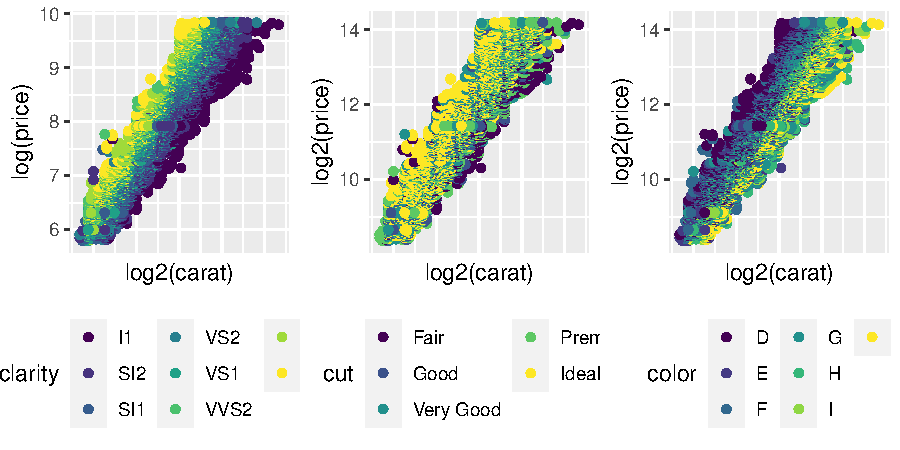
\includegraphics{Kor_AdvancedStats_files/figure-latex/unnamed-chunk-9-1} \end{center}

플롯에서 살펴볼 수 있는 이론적 기대와 경험적 관찰을 바탕으로, 저는 \texttt{price}를 설명하기 위한 선형회귀모델에 다이아몬드의 질을 보여주는 \texttt{clarity,\ cut,\ color}를 새로운 예측변수로 추가하기로 결정하였습니다. 그렇다면 모델에 새롭게 추가된 각 변수들은 앞의 단순선형모델의 잔차와 어떠한 관계를 맺고 있을까요?

\begin{center}\includegraphics{Kor_AdvancedStats_files/figure-latex/unnamed-chunk-10-1} \end{center}

\texttt{clarity,\ cut,\ color} 모두가 잔차와 상관이 있는 것 같습니다만. 우리는 단순선형회귀모델의 잔차로부터 체계적 요인---\texttt{clarity,\ cut,\ color}를 뽑아내어 \texttt{price}를 설명하기 위한 모델에 투입하기로 결정하였습니다.

\begin{Shaded}
\begin{Highlighting}[]
\NormalTok{mod_diamond3 <-}\StringTok{ }\KeywordTok{lm}\NormalTok{(}\DataTypeTok{formula=} \KeywordTok{log2}\NormalTok{(price) }\OperatorTok{~}\StringTok{ }\KeywordTok{log2}\NormalTok{(carat) }\OperatorTok{+}\StringTok{ }
\StringTok{                     }\NormalTok{clarity }\OperatorTok{+}\StringTok{ }\NormalTok{cut }\OperatorTok{+}\StringTok{ }\NormalTok{color, }\DataTypeTok{data=}\NormalTok{diamonds)}
\end{Highlighting}
\end{Shaded}

그리고 새롭게 구한 다중선형회귀모델, \texttt{mod\_diamond3}를 추정하고 그 결과로 얻은 잔차와 예측변수 \texttt{carat} 간의 관계를 살펴보았습니다.

\begin{center}\includegraphics{Kor_AdvancedStats_files/figure-latex/unnamed-chunk-12-1} \end{center}

다중선형회귀모델의 잔차와 로그값을 취한 \texttt{carat} 간에는 뚜렷한 경향성이 존재하는 것 같지는 않습니다. 이번에는 다이아몬드의 질을 보여주는 변수들과 다중선형회귀모델로 예측한 \texttt{price} 값 간의 관계를 플롯으로 보여보겠습니다.

\begin{center}\includegraphics{Kor_AdvancedStats_files/figure-latex/unnamed-chunk-13-1} \end{center}

네 개의 예측변수를 가지고 추정한 다중선형회귀모델로 그린 플롯은 상대적으로 단순선형회귀모델에서 충족시키지 못했던 선형회귀모델의 가정에 일부 부합하는 결과로 개선되었음을 확인할 수 있습니다. 먼저, 잔차는 로그값을 취한 \texttt{carat}과 체계적으로 상관하지 않습니다. 이는 잔차가 무작위로 분포되어 있다는 것을 의미합니다. 둘째, 예측된 \texttt{price}의 값과 다이아몬드 질 간의 관계는 관측된 \texttt{price} 값과 다이아몬드의 질 간의 관계와 유사한 양상을 보입니다. 이는 우리의 다중선형회귀모델이 주어진 예측변수들로 \texttt{price}를 잘 예측하고 있다는 것을 의미합니다.

\begin{center}\includegraphics{Kor_AdvancedStats_files/figure-latex/unnamed-chunk-14-1} \end{center}

그러나 이 모델은 충분하지 않습니다. 실질적으로 다이아몬드의 질을 보여주는 변수들은 주요 예측변수인 \texttt{carat}과 상관관계가 있음을 확인할 수 있기 때문입니다. 예를 들면, 가장 \texttt{clarity} 수준이 높은 다이아몬드는 극도로 그 크기(\texttt{carat})가 작은 것으로 나타납니다. 마찬가지로 \texttt{color}도 \texttt{carat}이 작을수록 높은 수준을 보여주고 있습니다. \texttt{Ideal}한 \texttt{cut} 다이아몬드는 전형적으로 작은 크기의 다이아몬드들에서 나타나고 있습니다.

위의 세 박스플롯들은 주요 예측변수 \texttt{carat}과 다른 다이아몬드의 질적 변수들 간의 상관성을 보여주고 있습니다. 즉, 이 네 예측변수를 이용한 다중선형회귀모델은 선형회귀모델의 기본적인 가정 중 하나인 예측변수들 간의 독립성을 심각하게 위배하고 있을 가능성을 시사합니다. 다이아몬드의 가격을 적절하게 예측하기 위해서는 예측변수들 간의 가산적 관계(additive relationship)를 가정하는 선형회귀모델을 새롭게 구축할 필요성이 있습니다.

또한 주요 예측변수와 종속변수에 로그값을 취했기 때문에 변수들 간의 정확한 효과를 직접적으로 해석하는 것은 어렵습니다. 애초에 원자료의 예측변수와 종속변수 간의 관계가 선형이지 않았기 때문에 그 둘의 관계를 로그값의 결과로 선형으로 해석할 수는 없기 때문입니다. 비록 변수에 로그를 취해서 선형회귀모델의 가정을 충족시켰다고는 하지만, 로그값을 취한 변수들을 사용한 모델의 결과를 통계적으로, 그리고 실질적으로 해석하는 것은 또 다른 문제입니다.

\hypertarget{basics-for-advanced-linear-regression-models-part-i}{%
\chapter{Basics for Advanced Linear Regression Models: Part I}\label{basics-for-advanced-linear-regression-models-part-i}}

앞서 우리가 이 \texttt{Lv.2.Statistics}에서 다룰 내용들을 위한 기본적인 개념들---함수, 도함수(derivatives), 자료의 유형, 추론, 변수, 그리고 척도 등에 대한 내용들을 이론적으로, 경험적으로 살펴보았습니다.

이제 여기에서는 \texttt{Lv.1.Statistics}에서도 다루었던 선형회귀모델에 대한 조금 더 깊이 들어간 내용들을 다루게 될 것입니다. 따라서 \texttt{Lv.1.Statistics}에서는 사실 예제를 통해서 훑고 지나갔단 선형회귀모델의 세부적인 구성요소들을 하나씩 짚어가면서 우리가 언제 선형회귀모델을 쓸 수 있고, 어떻게 해석할 수 있는지를 살펴볼 기초를 다져보겠습니다.

먼저, 간단한 함수적 관계를 나타내는 식이 있습니다. 이를 범죄의 모델(Model of Crime)이라고 해보겠습니다.
\[\text{범죄(Crime)} = f(\text{임금 수준(LW)})\]
위의 함수적 관계에서 각각의 항이 나타내는 것은 무엇일까요? 그리고 위의 관계는 우리에게 어떠한 것을 말해주고 있을까요? 위의 함수적 관계는 범죄(\texttt{Crime})의 변화량(variation)을 설명하는 데 있어서 임금 수준(\texttt{LW})이 중요하다는 것 밖에는 말해주지 않습니다. 이 모델을 가지고 우리는 그저 ``주로 임금 수준이 범죄를 설명하는 데 있어서 중요합니다''라고밖에 말할 수 없습니다. 어떻게, 얼마나 중요한지 위의 함수적 관계는 알려주지 않습니다. 다만 그 둘이 관계가 있다는 것만 시사합니다. 그렇다면 위의 함수적 관계를 조금 더 자세하게 풀어서 표현해보겠습니다.
\[\text{범죄(Crime)} = \beta_0 + \beta_1\text{임금 수준(LW)} + u\]
이제 우리에게 익숙한 선형모델의 형태로 나타납니다. 이 모델은 어떤 정보를 가지고 있을까요? 하나씩 뜯어보면, \(\beta_0 + u\)는 임금 수준이 0일 경우에 나타날 범죄율을 의미합니다. 그리고 임금 수준이 한 단위 증가할 때마다 범죄는 \(\beta_1\)만큼 증가하겠죠. 즉, 임금이 아예 없었을 경우의 범죄가 \(\beta_0 + u\)였다면, 임금이 한 단위 증가했을 때에는 \(\beta_0 + \beta_1\times1 + u = \beta_0 + \beta_1 + u\)가 되는 것입니다. 조금 더 자세히 뜯어보면,

\begin{itemize}
\tightlist
\item
  범죄(Crime): 종속변수(dependent variable)
\item
  임금(LW): 설명변수(explanatory variable)\footnote{저는 종속변수를 예측하기 위한 예측변수(predictor), 혹은 설명하기 위한 설명변수(explanatory variable)이라고 하고 독립변수(independent variable)라는 표현은 지양합니다. 왜냐하면 이 변수들이 외생적(exogeneous)이고 독립적이라는 근거는 어디에도 없기 때문입니다.}
\item
  \(\beta_0\): 임금이 0일 때의 범죄 수준
\item
  \(\beta_1\): 임금이 한 단위 변화할 때 나타나는 범죄의 변화
\item
  \(u\): 오차항(error term)
\end{itemize}

그렇다면 이 선형모델을 가지고 우리는 무엇을 할 수 있을까요? 바로 모델을 통해 우리가 관심을 가지고 있는 변수의 한 단위 변화와 연관되는 종속변수의 변화를 포착하는 것입니다. 한계효과(marginal effect)라고 하는데요, 단순선형회귀모델, 혹은 다중선형회귀모델에서는 각 변수들이 \texttt{+}로 결합되어 있습니다. 논리적으로 이 \texttt{+}는 서로가 독립적이라는 \texttt{OR}의 의미를 지니고 있습니다. 따라서 이와 같이 \texttt{+}로 변수들이 연결된 모델을 가산모형(additive models)이라고 하고, 이때의 한계효과는 각 변수들의 \(\beta_i\)라고 보시면 됩니다.

주어진 모델에서 한계효과를 수리적으로 나타내면 다음과 같습니다.
\[\text{Marginal effects:} \frac{\partial\text{(범죄)}}{\partial\text{(임금 수준)}} = \beta_1\]
그리고 이때 우리는 한계효과를 통해 특정한 임금 수준에서의 범죄 수준을 \textbf{예측}할 수 있게 됩니다.
\[\text{Predictions:} \hat{\text{범죄}} = \beta_0 + \beta_1\hat{\text{임금 수준}}\]

자, 그럼 차근차근 하나씩 구체적인 의미들을 살펴보겠습니다.

\hypertarget{beta_1uxc5d0-uxb300uxd558uxc5ec}{%
\section{\texorpdfstring{\(\beta_1\)에 대하여}{\textbackslash beta\_1에 대하여}}\label{beta_1uxc5d0-uxb300uxd558uxc5ec}}

다른 모든 조건들이 일정할 때(\emph{Ceteris paribus})라는 말이 있습니다. 통계방법에서는 다른 변수들의 효과를 실험실에서처럼 완벽하게 통제할 수 없기 때문에, 다른 변수들의 값을 동일하게 고정시켜둔 상태에서 우리가 관심을 가진 변수의 변화가 종속변수의 변화와 어떠한 관계에 놓여있는지를 살펴보게 됩니다. 따라서 \(\beta_1\)은 다른 모든 변수들이 동일한 값으로 고정되어 있을 때, 임금 수준의 값만 변화할 때 나타나는 범죄의 변화를 의미합니다.

그렇다면 \(u\)는 대체 무엇일까요? 이 모델에서 임금 수준과 \(u\)는 모두 확률변수입니다. 그리고 임금 수준이 변화하더라도 \(u\)는 변화하지 않습니다. \(u\)는 임금 수준으로 설명되지 않는 범죄의 나머지 부분으로, 우리가 관측하지 못하는(unobserved) 요소들입니다. 이론적으로는 \texttt{KKV}를 다시 한 번 불러와 그 개념대로 설명하면 이해가 쉽습니다. 우리는 종속변수, 범죄에 대해 체계적으로 연계되어 있을 것이라고 생각하고 체계적 요인(systematic factor)으로 임금 수준이라는 변수를 모델에 투입하였습니다. 그렇다면 우리의 이론적 기대가 다른 체계적 요인의 가능성을 제시하지 않는다면, 이론적으로는 범죄의 체계적 변화는 임금 수준으로 다 설명이 되고 체계적으로 설명되지 않는 비체계적 요인들만이 남게 될 것입니다. 이 비체계적 요인은 어떠한 경향성을 보이지 않는, 무작위(randamized)할 것이며 우리는 이를 확률변수(random variable)이라고 합니다. 마찬가지로 이 오차항---\(u\)는 설명변수와 \texttt{+}로 연결되어 있기 때문에 모델 안에서는 적어도 그들은 서로 관계가 없습니다(없어야만 합니다). 이를 수리적 공식으로 표현해보면 다음과도 같습니다.
\[E(u|x) = E(u)\]
주어진 \(x\)라는 조건에서 \(u\)의 기대값은 그냥 \(u\)의 기대값과도 같다, 즉 \(x\)는 \(u\)와 어떤 관계도 맺고 있지 않다는 것입니다. Wooldridge (2016: 22)는 ``\(\cdots\)우리는 관측할 수 없는 \(u\)가 설명변수 \(x\)와 관계되지 않도록 제한하는 가정을 만들었을 때만, 데이터의 무작위 표본(random sample)로부터 신뢰할 수 있는(reliable) 추정치, \(\beta_0, \beta_1\)을 확보할 수 있다.''고 언급하고 있습니다. 또한, ``그러한 제한이 없이 우리는 다른 조건들이 일정할 때의 효과 \(\beta_1\)를 추정할 수 없다''고 서술하고 있습니다.

여기서 하나 더 중요한 것이 바로 ``무작위 표본''이라는 것입니다. 무작위화(randomization)은 우리가 설명변수들과 오차항 간의 독립성 가정을 수립할 수 있도록 해주는 핵심적인 개념입니다. 만약 어떤 표본이 무작위로 뽑힌 것이 아니라 어떠한 기준에 의해서 뽑혔다면, 우리는 그 표본으로부터 얻은 결과가 실로 모집단에서의 관계를 보여주는지, 혹은 표본 선정에 관여한 기준으로 인해 나타난 경향성인지를 구분할 수 없을 것입니다.

\(x\)와 \(u\)에 대한 독립성 가정에 더해 Wooldridge (2016: 22)와 같이, 여기서도 \(u\)와 \(x\)가 어떻게 관계를 가지는지에 대한 가정을 별도로 수립하기 전까지는, 항상 \(u\)에 대하여 ``모집단에서의 \(u\)의 평균값은 0이다''라는 가정을 수립하도록 합니다. 이 가정은 \(E(u) = 0\)이라고 표현할 수 있습니다.

\hypertarget{euxuxc758-uxc758uxbbf8}{%
\subsection{\texorpdfstring{\(E(u|x)\)의 의미}{E(u\textbar x)의 의미}}\label{euxuxc758-uxc758uxbbf8}}

\(E(u|x)\)에 다시 한 번 살펴보겠습니다. \(E(u|x)\)는 \(x\)라는 설명변수가 주어진 조건 하에서의 \(u\), 오차항의 기대값을 보여주는 수리적 표현입니다. \(u, x\)가 확률변수이기 때문에, 우리는 \(x\)의 어떤 값이 주어졌다고 할 때의 \(u\)의 조건분포를 정의할 수 있습니다 (Wooldridge 2016: 22). 다른 표현으로는 \(x\)가 존재할 때의 \(u\)의 조건확률이라고 합니다. 단순선형회귀모델에서 우리는 이 조건확률을 0, \(E(u|x)=0\)이라고 가정합니다.
이론적으로 다시 한 번 살펴보았다면, 이번에는 좀 더 실질적인 맥락에서 이 가정을 살펴보겠습니다. 설명변수에 대한 오차항의 조건확률이 0이라는 것은 현실 속에서는 성립(혹은 충족)되기 어렵습니다. 왜냐하면 현실 속에서는 우리가 관측가능한 종속변수에 영향을 미칠 `수도' 있는 여러 `관측 불가능한' 혹은 `우리가 생각하지 못한' 잠재적 요인들이 존재할 수 있기 때문입니다.

또한, 우리가 모집단에 대한 회귀 함수(PRF)를 수립한다고 하더라도 우리가 확보 가능한 자료는 어디까지나 관측가능한 표본에 지나지 않습니다. 표본은 우리가 모집단에서 추출할 때마다 달라질 수 있고, 그것은 표본이 가지는 본연의 한계입니다. 따라서 어디까지나 표본을 사용한다는 점에서 우리는 본연적 불확실성에서 자유로울 수 없고, 이 오차항에 대한 가정은 충족되기 힘듭니다. 만약 이 오차항에 대한 가정이 심각하게 위배된다면, 우리는 그러한 표본으로부터 얻은 추정량들에 대해 ``편향되었다''(biased)라고 할 수 있을 것입니다.

논리적으로 \(\times\)는 \texttt{AND}로 두 가지 사건이 동시에 발생하였다는 것을 의미합니다. 그러나 이미 우리는 앞서 \(E(u)\)라고 가정한 바 있습니다. 따라서 어떤 \(x\)의 값이 주어지던 간에 상관없이, \(u\)의 기대값은 0이 됩니다. 이는 \(x\)와 \(u\)가 서로 독립적인 사건으로 \(u\)가 \(y\)와 \(x\)와 공변하지 않는다는 것을 의미합니다.

\begin{equation*}
\begin{aligned}
  Cov(x, u)& = E((x-\mu)(u-\nu)) = E(xu - x\nu - u\mu + \mu\nu)\\
  & = E(x\cdot u) - E(x\nu) - E(u\mu) + E(\mu\nu)\\
  & = E(x\cdot u) - \nu\mu - \mu\nu + \mu\nu\\
  & = E(x\cdot u) - \nu\mu\\
\end{aligned}
\end{equation*}

위의 수리적 유도에 따라 논리적으로 \(E(u|x)=Cov(x,u)=E(x\cdot u)\neq 0\)가 된다면, 설명변수는 종속변수에 영향을 미치는 오차항과 연관성이 있게 됩니다. 이 경우, 우리는 순수한 \(x\)와 \(y\)의 관계와 \(y\)에 대한 \(u\)의 관계를 구별해내기 어렵습니다. 이것이 \(x\)와 \(u\)가 서로 상관성이 있다고 할 때, 그 추정 결과가 편향된다고 말하는 근거입니다. 이렇게 여러 번 반복하는 이유는 그만큼 중요해서겠죠?

\hypertarget{uxbaa8uxc9d1uxb2e8-uxd68cuxadc0-uxd568uxc218population-regression-function-prf}{%
\section{모집단 회귀 함수(Population Regression Function; PRF)}\label{uxbaa8uxc9d1uxb2e8-uxd68cuxadc0-uxd568uxc218population-regression-function-prf}}

이전 자료에서 추론(inference) 파트에서 살펴보았듯, 우리가 관심있는 것은 표본에서의 변수들의 관계가 아닙니다. 우리는 어디까지나 그 표본이 모집단에 대해 대표성 있는 관측가능한 사례라고 간주하고, 그 표본에서의 관계가 관측불가능한 모집단에서도 유의미하게 나타날 것이라고 기대하는 것입니다. 따라서 어떠한 모델을 구성할 때, 우리는 두 가지 수준에서 모델을 생각해볼 수 있습니다. 바로 모집단 수준에서의 모델과 표본 수준에서의 모델입니다. PRF는 모집단 수준에서의 회귀모델을 의미합니다.
\begin{equation*}
\begin{aligned}
E(\text{범죄}|x, u)&= \beta_0 + \beta_1\text{임금 수준} + E(u|x)\\
&=\beta_0 + \beta_1\text{임금 수준}\\
&=E(\text{범죄}|x)
\end{aligned}
\end{equation*}
문제는 우리는 관측할 수 없지만 분명 존재할 \(\beta_0\)와 \(\beta_1\)에 대해 알고자 한다는 것입니다. 따라서 우리는 가지고 있는 데이터로부터 모집단의 \(\beta_0\)와 \(\beta_1\)을 추론할 필요가 있습니다. 그리고 표본에서 이 모집단의 \(\beta_0\)와 \(\beta_1\)을 보여주는 통계치(statistics)이자 예측치(estimates)는 \(\hat{\beta_0}\)와 \(\hat{\beta_1}\)라고 할 수 있습니다. 하지만 데이터만 가지고 잇을 때에는 \(\text{범죄}_i\)와 \(\text{임금 수준}_i\)라는 각 변수들의 개별 관측치들은 가지고 있는 것이지만 아직 그 두 변수의 관계를 보여주는 \(\beta_0\)와 \(\beta_1\)의 표본통계치, \(\hat{\beta_0}\)와 \(\hat{\beta_1}\)는 알지 못합니다.

\hypertarget{uxcd94uxc815-uxc870uxac74uxb4e4uxb4e4uxb85cuxbd80uxd130-uxb3c4uxcd9c}{%
\section{추정-조건들들로부터 도출}\label{uxcd94uxc815-uxc870uxac74uxb4e4uxb4e4uxb85cuxbd80uxd130-uxb3c4uxcd9c}}

여기에서는 두 가지 가정들을 살펴봅니다. 이 \(\beta_0\)과 \(\beta_1\)을 얻기 위해서는 이 두 가정들이 충족되어야 합니다. 하지만 관측된 자료들을 이용하는 연구에서는 사실 이 가정들이 모두 완벽하게 충족되기란 어렵습니다. 따라서 우리는 확보할 수 있는 데이터셋에 관해 매우 조심스러운 접근을 취할 필요가 있습니다. 과연 내가 가진 데이터는 이 두 가정을 충족시키는지, 그리고 충족시키지 않는다면 어떻게, 얼마만큼 위배하고 있는지를 면밀히 살펴보아야 합니다.

\hypertarget{uxac00uxc8151.uxacfc-uxc81cuxc57d1.}{%
\subsection{가정1.과 제약1.}\label{uxac00uxc8151.uxacfc-uxc81cuxc57d1.}}

제일 먼저 수립하는 가정과 그에 따른 제약은 바로 오차항의 기대값이 0으로 수렴한다는 것입니다. \(E(u) = 0\)으로 표현할 수 있겠죠? 그리고 오차항이 종속변수를 설명하기 위한 설명변수(\(x\))와 그 효과(\(\beta_1\)), 그리고 설명변수가 0일 경우의 값(\(\beta_0\))이라는 것을 감안할 때, 위의 가정은 다음과 같이 표현할 수 있습니다.
\begin{equation*}
\begin{aligned}
E(u)&= 0\\
&= E(y-\beta_0-\beta_1x)
\end{aligned}
\end{equation*}
모집단 수준에서의 오차항에 대한 가정이 다음과 같고, 이것이 참이라고 한다면, 개별 관측치로 나타나는 표본에서의 오차항에 대한 대응---잔차(residuals)에도 그와 같은 가정을 적용할 수 있을 것입니다.
\begin{equation*}
\begin{aligned}
E(u_i)&= 0\\
&= E(y_i-\hat{\beta_0}-\hat{\beta_1}x_i)
&= \frac{1}{N}\sum^{N}_{i=1}(y_i-\hat{\beta_0}-\hat{\beta_1}x_i) = 0
\end{aligned}
\end{equation*}
모집단에서 우리는 기대값(expected values)이라는 표현을 사용할 수 있지만, 표본 수준에서는 관측가능한 값, 평균(mean)으로 이를 보여줄 수 있습니다.

\hypertarget{uxac00uxc8152.uxc640-uxc81cuxc57d2.}{%
\subsection{가정2.와 제약2.}\label{uxac00uxc8152.uxc640-uxc81cuxc57d2.}}

두 번째 가정이란 설명변수와 오차항 간의 공변(covariation)이 존재하지 않는다는 것입니다. 즉, \(Cov(x, u)=0\)이라는 것이죠. 이것이 의미하는 게 무엇일까요?

\begin{equation*}
\begin{aligned}
E(u|x)&= Cov(x, u) = E(x\cdot u)=0\\
&=E(x(y=\beta_0-\beta_1x))
\end{aligned}
\end{equation*}

모집단 수준에서 주어진 설명변수가 있을 때의 오차항의 기대값은 곧 둘 간의 상관성을 묻는 것과 같습니다. 그리고 논리적 기호로써 이는 \(\times\)이며, \texttt{AND}고 둘이 서로 동시에 작동한다는 것을 의미합니다. 그럼 표본 수준에서 살펴볼까요?

\begin{equation*}
\begin{aligned}
E(u|x)&= 0\\
&= E(x_i(y_i=\hat{\beta_0}-\hat{\beta_1}x_i))\\
&= \frac{1}{N}\sum^{N}_{i=1}(x_i(y_i=\hat{\beta_0}-\hat{\beta_1}x_i)) = 0
\end{aligned}
\end{equation*}

이제 위의 두 가정들로부터 선형회귀모델의 \(\beta_0\)과 \(\beta_1\)을 추정하기 위한 \(\hat{\beta_0}\)과 \(\hat{\beta_1}\)을 얻는 과정을 유도해보도록 하겠습니다.

\hypertarget{uxc81c1uxb2e8uxacc4}{%
\subsubsection{제1단계}\label{uxc81c1uxb2e8uxacc4}}

가정 1(\(\frac{1}{N}\sum^{N}_{i=1}(y_i-\hat{\beta_0}-\hat{\beta_1}x_i)=0\))은 \(\bar{y}=\hat{\beta_0}+\hat{\beta_1}\bar{x}\)를 유도한다. 이때, \(\bar{x}\)와 \(\bar{y}\)는 각각 \(x\)와 \(y\)의 평균을 의미합니다.\footnote{\(\bar{x}\)와 \(\bar{y}\)는 주어진 표본에서의 특정한 ``수'', 평균입니다.} 즉, 선형회귀모델은 ``종속변수와 설명변수의 평균을 지나는'' 선을 그리게 됩니다. 위의 식에 따라 우리는 \(\hat{\beta_0} = \bar{y}-\hat{\beta_1}\bar{x}\)라는 결과를 얻을 수 있습니다.

\hypertarget{uxc81c2uxb2e8uxacc4}{%
\subsubsection{제2단계}\label{uxc81c2uxb2e8uxacc4}}

가정 2는 표본에서의 설명변수와 오차항 간 공변이 없을, \(\sum^{N}_{i=1}(x_i(y_i=\hat{\beta_0}-\hat{\beta_1}x_i)) = 0\)를 의미합니다. 그리고 이 경우, 식을 풀어서 \(\sum^{N}_{i=1}x_i(y_i-\bar{y})=\hat{\beta_1}\sum^{N}_{i=1}x_i(x_i-\bar{x})\)로 표현할 수 있습니다. 여기서부터는 수리적으로 계속 유도해내는 거라서 굳이 하나하나 다 이해하실 필요가 있다고는 하지 않겠습니다만, 다시 쓰면\(\cdots\)
\(\sum^{N}_{i=1}x_i(y_i-\bar{y})=\sum^{N}_{i=1}(x_i-\bar{x})(y_i-\bar{y})\)로 보여줄 수 있고, \(\sum^{N}_{i=1}x_i(_i-\bar{x})=\sum^{N}_{i=1}(x_i-\bar{x})^2\)라고 할 수 있습니다. 결론적으로 이 일련의 복잡한 식들을 통해서 우리는 앞의 \(\hat{\beta_0}, \hat{\beta_1}\)에 대입, 이 두 통계치를 \(x\)와 \(y\)로 보여줄 수 있습니다.
\begin{equation*}
\begin{aligned}
&\hat{\beta_1}=\frac{\sum^{N}_{i=1}(x_i-\bar{x})(y_i-\bar{y})}{\sum^{N}_{i=1}(x_i-\bar{x})^2}\\
&\hat{\beta_0} = \bar{y}-\hat{\beta_1}\bar{x}
\end{aligned}
\end{equation*}

\hypertarget{uxc5b8uxc81c-beta_1uxc758-uxac12uxc774-uxcee4uxc9c8uxae4c}{%
\subsection{\texorpdfstring{언제 \(\beta_1\)의 값이 커질까?}{언제 \textbackslash beta\_1의 값이 커질까?}}\label{uxc5b8uxc81c-beta_1uxc758-uxac12uxc774-uxcee4uxc9c8uxae4c}}

\(\beta_1\)은 간단히 얘기하면 기울기, \(x\)와 \(y\) 간의 관계 양상을 보여주는 추정치입니다. 그런데 이 \(\beta_1\)을 추론하기 위하여 우리가 구하는 표본의 통계치, \(\hat{\beta_1}\)은 자료의 척도(scale)와 밀접하게 관련되어 있습니다. Wooldridge (2016: 26)에서 \(\hat{\beta_1}\)를 구하기 위한 공식을 \(\hat{\beta_1} = \hat{\rho}_xy\cdot \frac{\hat{\sigma}_y}{\hat{\sigma}_x}\)이라고 보여주고 있습니다. 이것이 의미하는 것은 무엇일까요? 만약 \(y\)의 척도, 단위가 \(x\)의 척도, 단위에 비해 훨씬 크다면, \(\hat{\beta_1}\)는 상대적으로 매우 커진다는 것을 의미합니다. 분수니까요. \(x\)의 분산이 \(y\)의 분산보다 훨씬 작을 경우에도 마찬가지로 상대적으로 큰 \(\hat{\beta_1}\) 값을 가질 수 있다는 것을 보여줍니다.

\hypertarget{uxcd94uxc815-uxc794uxcc28uxc758-uxcd5cuxc18cuxd654}{%
\section{추정-잔차의 최소화}\label{uxcd94uxc815-uxc794uxcc28uxc758-uxcd5cuxc18cuxd654}}

위에는 \(\beta_0, \beta_1\)을 추정하기 위한 \(\hat{\beta_0}, \hat{\beta_1}\)을 구하기 위해 필요한 두 가지 가정을 살펴보았습니다. 이번에는 또 다른 관점에서 \(\hat{\beta_0}, \hat{\beta_1}\)을 살펴보겠습니다.

\begin{itemize}
\item
  예측값(fitted values): 주어진 설명변수 \(x\)를 우리가 구한 \(\hat{\beta_0}, \hat{\beta_1}\)에 대입하여 종속변수를 예측한 값입니다. \(\hat{y_i} = \hat{\beta_0} + \hat{\beta_1}x_i + \hat{u}_i\)라고 할 수 있습니다.
\item
  잔차(Residuals, \(\hat{u}_i\))는 모집단의 오차항 \(u\)와 대응되는 표본통계치입니다.
\item
  잔차/오차항이란 우리가 예측하지 못한, 혹은 관측하지 못한 것---불확실성입니다. 불확실성을 가능한 한 줄이는 것은 어찌보면 사회과학의 본령일지도 모릅니다.

  \begin{itemize}
  \tightlist
  \item
    잔차의 평균이 0이라고 했기 때문에 단순하게 이 잔차들을 더한 값을 최소화하는 것은 의미가 없습니다. 비체계적 요인들이 서로 상쇄(offsets)된다고 할 때, 잔차를 최소화하는 방법은 크게 두 가지가 있을 것입니다. 절대값을 구해서 그 모든 절대값들의 합이 최소가 되게 하는 것, 그리고 제곱의 합이 최소가 되게 하는 것입니다. 이 둘의 차이는 개념적으로는 없습니다. 다만 후자---제곱합이 수리적으로 더 계산이 용이하기 때문에 이 방법을 택하는 것일 뿐입니다.
  \end{itemize}
\item
  잔차의 제곱합을 최소화하는 것은 앞서 가정들에서 \(\hat{\beta_0}, \hat{\beta_1}\)을 도출해낸 것과 같은 결과로 이어집니다.
\end{itemize}

\hypertarget{uxd45cuxbcf8-uxd68cuxadc0-uxd568uxc218-sample-regression-function-srf}{%
\subsection{표본 회귀 함수 (Sample regression function, SRF)}\label{uxd45cuxbcf8-uxd68cuxadc0-uxd568uxc218-sample-regression-function-srf}}

표본 회귀 함수는 모집단의 모집단 회귀 함수와 동일한 형태를 가집니다(\(\hat{y}=\hat{\beta_0}+\hat{\beta_1}x\)). 함수적 관계라는 측면에서는 \(\hat{y} = f(x, \hat{\beta_1}, \hat{\beta_0})\)라고도 표현할 수 있습니다. 우리는 이 표본 회귀 함수를 가지고 도함수(편미분) 등을 통해 우리가 원하는 결과들을 확인할 수 있습니다.

한 번 앞의 범죄-임금 수준 함수를 가지고 살펴보겠습니다. \(y\)가 범죄, \(x\)가 임금 수준이라고 하고 \(\hat{\beta_0}=11, \hat{\beta_1}=-0.5\)라고 해봅시다.

\begin{itemize}
\item
  우리는 \(x\)가 20일때와 2일 때의 예측값의 차이도 살펴볼 수 있고; \(f(x=20, \cdot) - f(x = 2, \cdot)\)
\item
  도함수를 통해서 한계효과를 계산할 수도 있으며; \(\frac{\partial f(x, \cdot)}{\partial x}\)
\item
  \(x\)가 0일 때의 \(y\)의 값을 구할 수도 있고; \(f(x = 0, \cdot)\)
\item
  변화율을 살펴볼 수도 있습니다; \(\frac{f(x=20, \cdot) - f(x = 2, \cdot)}{f(x = 2, \cdot)}\times100\)
\end{itemize}

\hypertarget{uxbaa8uxc9d1uxb2e8-uxd68cuxadc0-uxd568uxc218uxc640-uxd45cuxbcf8-uxd68cuxadc0-uxd568uxc218uxc758-uxc774uxd574}{%
\section{모집단 회귀 함수와 표본 회귀 함수의 이해}\label{uxbaa8uxc9d1uxb2e8-uxd68cuxadc0-uxd568uxc218uxc640-uxd45cuxbcf8-uxd68cuxadc0-uxd568uxc218uxc758-uxc774uxd574}}

이쯤에서 한 번 내용들을 정리하고 넘어가겠습니다. \(\beta_0, \beta_1, \hat{\beta_0}, \hat{\beta_1}, x, x_i, u, \hat{u_i}\), 그리고 \(\bar{x}\)와 같이 여러 가지 수리적 표현들이 등장했는데요, 이들 각각은 대체 무슨 의미를 지니고 있는 걸까요? 그리고 이 각각의 값들은 \textbf{확정적(fixed)}인걸까요 아니면 \textbf{확률적(random)}일까요? 이를 설명하기 위해서는 모집단과 표본의 관계에 대한 명확한 관점이 필요합니다.

우리는 모집단과 표본을 구별해야만 합니다. 그리고 모집단 회귀 모델과 표본 회귀 모델 역시 구분해야 합니다. 비록 우리가 모집단에 관심을 가지고 있다고 하더라도 현실 속에서 우리가 가질 수 있는 것은 오직 표본입니다. 따라서 우리는 관측불가능한 모집단의 특성들을 관측가능한 표본들을 통해서 추론하고자 합니다. 이는 이론적으로 모집단에 대해 우리가 관심을 가지는 값들---모수(parameters)는 이미 주어진 것들로 확정정인 값들이라는 것을 의미하며, 표본의 통계치들은 모집단에서 추출하는 과정 속에서 불확실성을 내재하게 되므로 표본에 따라 다르게 나타날 수 있습니다. 즉, 확률적입니다.

\begin{itemize}
\item
  PRF는 모집단의 수준에서 어떠한 함수적 관계를 가지고 하나의 설명변수가 종속변수와 관계되어 있다고 가정할 때, 두 가지 모수를 구할 수 있다는 것을 보여줍니다. 바로 \(\beta_0\)와 \(\beta_1\)입니다.

  \begin{itemize}
  \item
    \(\beta_0\)는 절편에 대한 모수값입니다. 우리가 상정한 설명변수의 값이 0일 때의 종속변수의 값을 보여주는 것이죠. 모집단의 속성을 보여주는 이 \(\beta_0\)은 모집단 수준에서는 확정적인 값입니다.
  \item
    \(\beta_1\)은 기울기에 대한 모수값입니다. \(\beta_1\)은 다른 모든 조건들이 일정할 때, \(x\)와 \(y\) 간의 관계를 보여줍니다. \(\beta_0\)와 마찬가지로 확정적인 값입니다.
  \item
    \(u\)은 관측되지 않았지만 종속변수에 영향을 미칠 것으로 기대되는 요인들입니다. 따라서 \(u\)는 \(x\)에 의해 설명되지 않는 \(y\)의 일부라고 표현할 수 있습니다. 하지만 이 \(u\)는 비체계적이고 확률적이기 때문에 서로 상쇄되어 0으로 수렴할 것이라고 가정할 수 있습니다. 모집단의 수준에서는 확률변수이지만 동시에 이 오차항도 고정된 값입니다. 0으로 수렴하는 고정된 값이지요.
  \item
    \(x\)는 종속변수를 설명할 것으로 기대되는 변수로 마찬가지로 모집단 수준에서는 확정적인 값을 가집니다. 종속변수 \(y\)도 마찬가지겠죠?
  \end{itemize}
\item
  SRF는 표본 회귀 함수로 PRF와 같은 형태를 취하지만 다만 표본 수준의 논의라는 점이 다를 뿐입니다.

  \begin{itemize}
  \item
    \(\hat{\beta_0}, \hat{\beta_1}\)은 모수값, \(\beta_0, \beta_1\)을 추정하기 위해 구한 표본에서의 추정치입니다. \(\hat{\beta_0}\)은 절편에 대한 통계치이며 \(\hat{\beta_1}\)은 기울기에 대한 표본의 통계치입니다. 따라서 이 값들은 표본을 어떻게 뽑느냐에 따라서 매번 달라질 수 있으므로 ``확률적''인 값들입니다.
  \item
    \(x_i, \hat{u_i}\)은 각각 설명변수의 개별 관측값들과 주어진 설명변수 값에 대한 예측된 종속변수의 값과 실제 관측된 종속변수 값의 차이를 의미합니다. \(u_i\)는 \(y_i - \hat{y}\)라고 할 수 있습니다. 두 값 모두 표본 수준의 논의이므로 확률적인 값들입니다.
  \item
    \(\bar{x}\)는 표본에서 관측된 설명변수의 평균으로 표본에 따라 달라집니다. \(\bar{y}\)도 마찬가지로 표본의 종속변수 평균이며 표본에 따라 달라지므로, 이 두 값 모두 확률적인 값들입니다.
  \end{itemize}
\end{itemize}

\hypertarget{uxc77cuxc885uxc758-uxcd1duxd569uxb4e4-sums}{%
\subsection{일종의 ``총합들'' (sums)}\label{uxc77cuxc885uxc758-uxcd1duxd569uxb4e4-sums}}

우리는 다양한 종류의 제곱합들을 통해 회귀모델의 특성을 보여줄 수 있습니다.

\begin{itemize}
\item
  총 제곱합(Total sums of squares): SST = \(\sum^{N}_{i=1}(y_i-\bar{y})^2\)
\item
  설명된 변동량의 제곱합(Explained sums of squares): SSE = \(\sum^{N}_{i=1}(\hat{y_i}-\bar{y})^2\)
\item
  잔차의 제곱합(Residual sums of squares): SSR = \(\sum^{N}_{i=1}(\hat{y_i}-y_i)^2\)
\item
  모델이 얼마나 잘 들어맞는지를 보여주는 측정지표인 결정계수, \(R^2 \equiv \frac{SSE}{SST}\)
\end{itemize}

이같은 변동량에 대한 논의는 \(y\), \(x\), 그리고 \(u\)에 대한 벤다이어그램을 통해 도식적으로도 보여줄 수 있습니다. 물론 변수가 많아질수록 이렇게 도식화하는 것은 점점 어려워지기는 합니다. 그러나 여기서는 단순선형회귀모델을 가정하고 간단한 그림을 그려보겠습니다.
\newpage

\begin{Shaded}
\begin{Highlighting}[]
\NormalTok{knitr}\OperatorTok{::}\KeywordTok{include_graphics}\NormalTok{(}\StringTok{"figures/Venndiagram.png"}\NormalTok{)}
\end{Highlighting}
\end{Shaded}

\begin{center}\includegraphics[width=7.88in]{figures/Venndiagram} \end{center}

벤다이어그램은 \(y\), \(x\), 그리고 \(u\)에 대한 단순선형회귀모델에서의 설명력을 묘사하고 있습니다. 먼저, 붉은 영역은 \(x\)를 가지고 설명되는 \(y\)의 변동량이라고 할 수 있습니다. 단순선형회귀모델에서 하나의 설명변수가 \(y\)를 설명할 것이라고 기대하더라도 우리는 그것이 \(y\)의 전체 변화를 설명할 수 있다고 단언할 수는 없습니다. Wooldridge의 표현대로라면 벤다이어그램에서 오른쪽이 ``설명된 변동량의 제곱합''(Explained sum of squares, SSE)이며, 왼쪽이 잔차의 제곱합(Residual sum of squares, SSR)이라고 할 수 있습니다.

\hypertarget{ruxb85c-uxacc4uxc0b0uxd574uxbcf4uxae30}{%
\subsection{\texorpdfstring{\textbf{R}로 계산해보기}{R로 계산해보기}}\label{ruxb85c-uxacc4uxc0b0uxd574uxbcf4uxae30}}

앞에서의 이론적 논의들을 한 번 \textbf{R}을 통해 경험적 데이터를 가지고 계산해보도록 하겠습니다. 구체적으로는 주어진 데이터로 \(\hat{\beta_0}, \hat{\beta_1}\), 그리고 \(R^2\)를 구해볼 겁니다.

예제로 사용할 데이터는 2016년도 국가 수준의 집합자료들입니다. 사실 교차사례-시계열 자료로 구축할 수도 있지만 그렇게 되면 너무 복잡하니까 2016년도를 따로 떼어내서 교차사례 자료로 만들었습니다. 이 자료에서 국가의 노령화 정도와 경제 간의 관계에 관심을 가지고 있다고 하겠습니다.

분석단위는 따라서 국가가 되겠고, 노령화 수준이 높은 국가일수록 생산성이 낮아져서 경제 수준도 낮을 것이라는 이론적 기대를 가지고 모델을 만들어보겠습니다. 물론, 원래 모델을 구성하려면 더 세심한 고려가 필요하겠습니다만, 여기서는 \textbf{R} 예제를 보이는 것이 목표이니만큼 단순화된 모델 구축으로 넘어가겠습니다. 여하튼, 이 예제에서 상정된 이론적 모델은 다음과 같습니다: \(\text{경제수준} = \beta_0 + \beta_1\text{(노령화 수준)} + u\).

분석을 위해 사용한 자료는 \texttt{The\ Quality\ of\ Government\ Basic\ Dataset} 입니다. 주요 변수로는 2016년도의 2010년 미국 달러 고정으로 계산된 1인당 GDP(\texttt{wdi\_gdpcapcon2010})와 노동가능인구 대비 노인 인구로 계산된 노령화 지수(\texttt{wdi\_agedr})입니다.

\begin{itemize}
\item
  먼저, 1인당 GDP는 는 국내총생산을 그 해 중간의 인구 수로 나눈 값이기 때문에 단순 GDP 보다는 국가의 경제 규모를 더 잘 보여주는 지표라고 판단하여 사용하였습니다. 인구 100만명인데 100만 달러 버는 나라와 1000만명인데 300만 달러를 버는 나라를 비교해보았을 때, 후자가 더 부유하다고 단순하게 말하기는 어려울 겁니다.
\item
  그 다음으로 생산성에 있어서 노령 인구가 젊은 인구에 비해서 더 낮을 것이라고 볼 수 있기 때문에 노령인구 수준이 더 높을수록 경제 수준이 더 낮을 것이라고 기대합니다. 따라서 노령인구 비율은 노동 가능인구에 대해 측정됩니다. 노동가능인구는 약 15세에서 64세 사이의 인구이며, 노령인구는 64세 초과의 인구입니다.
\end{itemize}

\begin{Shaded}
\begin{Highlighting}[]
\KeywordTok{library}\NormalTok{(ezpickr)}
\KeywordTok{library}\NormalTok{(tidyverse)}
\NormalTok{QOG <-}\StringTok{ }\KeywordTok{pick}\NormalTok{(}\DataTypeTok{file =} \StringTok{"http://www.qogdata.pol.gu.se/data/qog_bas_ts_jan19.dta"}\NormalTok{)}
\NormalTok{QOG_summary <-}\StringTok{ }
\StringTok{  }\NormalTok{QOG }\OperatorTok\StringTok{ }\KeywordTok{select}\NormalTok{(ccodecow, cname, year, }
\NormalTok{                 wdi_agedr, wdi_gdpcapcon2010) }\OperatorTok
\StringTok{  }\NormalTok{dplyr}\OperatorTok{::}\KeywordTok{filter}\NormalTok{(year}\OperatorTok{==}\DecValTok{2016}\NormalTok{) }\OperatorTok\StringTok{ }\KeywordTok{drop_na}\NormalTok{()}

\NormalTok{y <-}\StringTok{ }\NormalTok{QOG_summary}\OperatorTok{$}\NormalTok{wdi_gdpcapcon2010}
\NormalTok{x <-}\StringTok{ }\NormalTok{QOG_summary}\OperatorTok{$}\NormalTok{wdi_agedr}
\NormalTok{model <-}\StringTok{ }\KeywordTok{lm}\NormalTok{(y }\OperatorTok{~}\StringTok{ }\NormalTok{x, }\DataTypeTok{data=}\NormalTok{QOG_summary)}
\NormalTok{b1.hat <-}\StringTok{ }\NormalTok{(}\KeywordTok{sd}\NormalTok{(y) }\OperatorTok{/}\StringTok{ }\KeywordTok{sd}\NormalTok{(x)) }\OperatorTok{*}\StringTok{ }\KeywordTok{cor}\NormalTok{(y, x)}
\NormalTok{b0.hat <-}\StringTok{ }\KeywordTok{mean}\NormalTok{(y) }\OperatorTok{-}\StringTok{ }\NormalTok{b1.hat }\OperatorTok{*}\StringTok{ }\KeywordTok{mean}\NormalTok{(x)}
\NormalTok{y.hat <-}\StringTok{ }\NormalTok{b0.hat }\OperatorTok{+}\StringTok{ }\NormalTok{b1.hat }\OperatorTok{*}\StringTok{ }\NormalTok{x }\CommentTok{# 주어진 x로 예측한 y의 예측값들}
\NormalTok{SSE <-}\StringTok{ }\KeywordTok{sum}\NormalTok{((y.hat }\OperatorTok{-}\StringTok{ }\KeywordTok{mean}\NormalTok{(y))}\OperatorTok{^}\DecValTok{2}\NormalTok{)}
\NormalTok{SSR <-}\StringTok{ }\KeywordTok{sum}\NormalTok{((y }\OperatorTok{-}\StringTok{ }\NormalTok{y.hat)}\OperatorTok{^}\DecValTok{2}\NormalTok{)}
\NormalTok{R2 <-}\StringTok{ }\NormalTok{SSE }\OperatorTok{/}\StringTok{ }\NormalTok{(SSE }\OperatorTok{+}\StringTok{ }\NormalTok{SSR) }
\KeywordTok{round}\NormalTok{(b1.hat, }\DecValTok{3}\NormalTok{)}
\end{Highlighting}
\end{Shaded}

\begin{verbatim}
## [1] -418.258
\end{verbatim}

\begin{Shaded}
\begin{Highlighting}[]
\KeywordTok{round}\NormalTok{(b0.hat, }\DecValTok{3}\NormalTok{)}
\end{Highlighting}
\end{Shaded}

\begin{verbatim}
## [1] 38207.65
\end{verbatim}

\begin{Shaded}
\begin{Highlighting}[]
\KeywordTok{round}\NormalTok{(R2, }\DecValTok{3}\NormalTok{)}
\end{Highlighting}
\end{Shaded}

\begin{verbatim}
## [1] 0.148
\end{verbatim}

각각의 결과들을 한 번 살펴보고 해석해볼까요? 편의상 소수점 없이 정수로만 나타내겠습니다.

\begin{itemize}
\item
  먼저 \(\hat{\beta_1}\)은 약 -418.258로 노령화 비율이 한 단위 증가할수록 \(\hat{\beta_1}\)만큼 1인당 GDP가 감소할 것이라는 것을 보여줍니다.
\item
  \(\hat{\beta_0}\)는 38207.65로 \(x\), 노령화 비율이 0일 때의 1인당 GDP의 규모를 보여줍니다.
\item
  그렇다면 모델의 설명력은? \(R^2\)로 볼 수 있습니다. 약 0.187이네요. 비율이니까 다시 말하면, 노령화 비율로는 1인당 GDP의 변화를 약 14.8\% 설명할 수 있다, 이렇게 이해하실 수 있을 것 같습니다. 한편, 이것은 단순하게 1인당 GDP의 평균으로 1인당 GDP의 변화를 설명하는 것보다 더 나은 설명력을 모델이 제공한다는 것을 의미합니다.
\end{itemize}

또, 척도에 따라 이 \(\beta_1\)의 값이 민감하게 변화한다는 것을 언급했었는데요. 이번에는 주어진 SRF, \(\hat{y} = \hat{\beta_0} + \hat{\beta_1}x + \epsilon\)에서 설명변수 \(x\)에 로그값을 취한 다른 측정척도의 \(z\)를 모델에 투입해보겠습니다.

\begin{itemize}
\item
  앞서 1인당 GDP와 노령화 비율로 구성한 SRF에 따르면, \(x\) 한 단위의 변화는 \(\hat{\beta_1}\)만큼의 종속변수 변화와 관계가 있습니다. 그리고 종속변수의 예측값은 \(x=1\)일 때, \(\hat{y} = \hat{\beta_0 + \hat{\beta_1}}\)로 나타낼 수 있습니다. 마찬가지로 \(x=2\)일 때는 \(\hat{y} = \hat{\beta_0} + 2\hat{\beta_1}\)로 보여줄 수 있고, \(x=1\)일 때와 \(x=2\)일 때의 차이가 \(\hat{\beta_1}\)입니다.
\item
  그렇다면 만약 \(z\)를 투입하게 되면, \(z\) 한 단위의 변화가 종속변수의 변화와는 어떤 관계를 맺게 될까요? 도식적으로 보면 다음과 같을 겁니다. \(y = \hat{\beta_0} + \hat{\beta_1}\text{log}x\).

  \begin{itemize}
  \item
    이 경우에는, \(y + \partial y = \hat{\beta_0} + \hat{\beta_1}\text{log}(x + \partial x)\)라 할 수 있고,
  \item
    좀 더 자세하게는 아래와 같이 표현할 수 있습니다.
  \end{itemize}
\end{itemize}

\begin{equation*}
\begin{aligned}
  \partial y&= \hat{\beta_1}(\text{log}(x + \partial x) - \text{log}x)\\
   &= \hat{\beta_1}\text{log}(1 + \frac{\partial x}{x})
\end{aligned}
\end{equation*}

만약 \(\frac{\partial x}{x}\) is 작다면, t\(\text{log}(1 + \frac{\partial x}{x}) \approx \frac{\partial x}{x}\)일 거라고 생각해볼 수 있습니다.

여기서 우리는 \(x\)의 1퍼센트 변화가 \(y\)의 \(\frac{\hat{\beta_1}}{100}\)만큼의 변화와 관계가 있을 것이라고 이해할 수 있습니다. 즉, 변수의 측정척도는 연구에 있어서 중요합니다. 실질적으로 단순히 변화량을 보여주는 것만이 아니라 때로는 변화율을 보여주는 것이 실질적으로 더 많은 정보를 제공할 수 있습니다.

\(x\)에 로그값을 취하면 우리는 \(x\)의 한 단위 변화가 아니라 1\% 변화가 \(y\)에 미치는 효과를 볼 수 있게 됩니다: \(\frac{\hat{\beta_1}}{100}\). 예를 들어, \(x\)가 연간 소득이라고 할 때, 사실 우리는 연간 소득의 1달러 변화가 궁금하다기 보다는 연간 소득의 비율 변화가 \(y\)와 어떠한 관계가 있는지 궁금할 것입니다. 따라서 연구목적에 따라 우리는 측정척도들을 변화시킬 수 있으며, 주의해야할 것은 그 경우 변화된 척도에 맞춰 해석해줘야 한다는 것입니다.

\hypertarget{basics-for-advanced-linear-regression-models-part-ii}{%
\chapter{Basics for Advanced Linear Regression Models: Part II}\label{basics-for-advanced-linear-regression-models-part-ii}}

단순선형회귀모델은 단순해보이지만 결코 단순하지 않습니다. 앞에서 우리는 \texttt{+}가 각 변수들 간의 독립적인 관계를 보여준다는 것을 확인하였습니다. 이번에는 범죄에 대한 회귀모델을 구축하되, 임금 수준 이외의 또 다른 변수---경찰의 노력(Police effort)를 포함해봅시다. 선형회귀모델이되 둘 이상의 설명변수를 포함하였으니 다중선형회귀모델(multiple linear regression model)이라고 할 수 있을 것입니다. 통계적 모델로 나타내자면 \(\text{범죄} = \beta_0 + \beta_1\text{임금 수준} + \beta_2\text{경찰의 노력} + u\)가 될 것입니다.

우리는 일단 다중선형회귀모델의 각 계수, \(\beta_i\)들을 어떻게 구할 수 있는지를 살펴볼 것입니다. 그리고 설명변수로서의 제곱항(square term)이 포함된 다중선형회귀모델에서 \(\beta_i\)가 가지는 의미를 분석하고자 합니다.다중선형회귀모델 통계적 특성은 다음과 같습니다.

\begin{itemize}
\item
  MLR.1: 모수들은 선형관계를 이루고 있다.
\item
  MLR.2: 표본은 무작위로 추출된 것이다(random sampling)
\item
  MLR.3: 완전한 다중공선성은 존재하지 않아야 한다(No perfect collinearity)
\item
  MLR.4: 오차항과 설명변수들 간의 상관관계가 존재하지 않아야 한다(\(E(u|x_i,\cdots,x_k) = 0\)).
\end{itemize}

우리는 MLR.1부터 MLR.4까지를 가정하고, \(y_i = \hat{\beta_0} + \hat{\beta_1}x_{i1} + \hat{\beta_2}x_{i2}\)를 가정합니다. 따라서 다중선형회귀모델에서 \(\hat{\beta_1}\)을 구하기 위해서는 다음과 같은 공식이 성립합니다.
\[\hat{\beta_1} = \frac{\sum^{n}_{i=1}\hat{r}_{i1}\cdot y_i}{\sum^{n}_{i=1}\hat{r}^2_{i1}}\]
이때, \(r_{i1}\)은 잔차로 \(x_{i1} = \hat{\alpha}_0 + \hat{\alpha}_1x_{i2} + r_{i1}\)에서 도출된 것입니다. 간단히 말하자면, 단순선형회귀모델에서와는 달리 다중선형회귀모델에서는 \(\hat{\beta_1}\)을 구할 때, \(x_1\)과 \(y\) 간의 관계뿐 아니라 \(x_1\)과 \(x_2\) 간의 관계, 그리고 \(x_2\)와 \(y\)의 관계도 고려해주어야 한다는 것입니다. 왜? \(x_1\)이 설명하고 있는 부분의 일부는 사실 \(x_1\)과 \(x_2\)가 같이 설명하는 ``교집합'', ``공분산''(covariance)일 수 있기 때문입니다.

공분산에 대한 내용은 뒤에서 더 자세하게 다루기로 하고, 우선 MLR.1부터 MLR.4까지의 가정들이 모두 충족되었을 때, 우리는 수없이 많은 표본들로부터 얻어내는 \(\hat{\beta}_k\)의 기대값이 모집단에서의 \(\beta_k\)와 같을 것이라고 생각할 수 있습니다: \(E(\hat{\beta}_k) = \beta_k\). 이를 최소자승법으로 구한 선형회귀모델의 계수값의 비편향성(unbiasedness)라고 합니다.

\hypertarget{uxc624uxcc28errors}{%
\section{오차(Errors)}\label{uxc624uxcc28errors}}

이번에는 오차에 대해서 배워보겠습니다. 앞서 우리는 모집단 수준에서의 오차의 기대값은 0으로 수렴한다(\(E(u) = 0\))는 것을 가정하였습니다. 그렇다면 오차의 분산(\(Var(u)\))은 어떨까요? 이 오차의 분산에 관한 내용이 바로 다중선형회귀모델의 다섯번째 통계적 특성이자 가정, MLR.5입니다.

\begin{itemize}
\item
  MLR.5: 오차의 분산은 동질적이다(Homosckedasticity).

  \begin{itemize}
  \item
    \(Var(u|x_i, \cdots, x_k)=\sigma^2\)
  \item
    \(E(y|x_1, x_2) = \beta_0 + \beta_1x_1 + \beta_2x_2\)
  \item
    \(Var(y|x_1, x_2) = Var(y) = Var(u) = \sigma^2 = E(u^2)\)
  \item
    오차의 표준편차는 \(\sqrt{\sigma^2} = \sigma\)가 됩니다.
  \end{itemize}
\item
  위에서부터 순서대로 저 가정의 내용을 풀어가보면, 먼저 우리는 주어진 설명변수들 하에서 오차항의 분산을 모집단 수준에서 \(\sigma^2\)라고 합니다. \(\sigma\)가 표준편차고 분산은 표준편차의 제곱이라는 수리적 정리를 여기서 딱히 증명할 필요는 없을 거 같으니 이렇게 넘어가겠습니다.
\item
  그리고 \(x_1, x_2\)라는 다중선형회귀모델의 두 설명변수가 있다고 할 때, 그 설명변수들이 주어졌을 때의 종속변수를 예측할 수 있는 기대값은 오차를 제외한 두 설명변수의 다중선형회귀모델의 PRF로 결정됩니다.
\item
  그리고 이러한 설명변수들이 주어졌을 때의 종속변수의 분산은 MLR.5에 따라 오차항의 분산과 같고, 오차항의 분산은 \(\sigma^2\)입니다. 이는 \(u^2\)의 기대값과도 같습니다.
\item
  표준편차는 분산의 제곱근이므로 결과적으로 오차의 표준편차는 \(\sigma\)가 됩니다.
\end{itemize}

\hypertarget{hatsigma2-uxcd94uxc815uxd558uxae30}{%
\subsection{\texorpdfstring{\(\hat{\sigma}^2\) 추정하기}{\textbackslash hat\{\textbackslash sigma\}\^{}2 추정하기}}\label{hatsigma2-uxcd94uxc815uxd558uxae30}}

표본에서의 오차---즉, 잔차의 분산(\(\hat{\sigma}^2\))은 표본의 크기의 영향을 받습니다. 정확히는 \[\hat{\sigma}^2=\frac{1}{n-K-1}\sum\hat{u}^2_i\]이며, 이는 곧 잔차의 제곱합을 n-k-1, 전체 관측치의 개수에서 변수의 개수-1을 하는 것과 같습니다(\(SSR/(n-K-1)\)).

MLR.1부터 MLR.5까지의 가정이 모두 충족된다면 모집단 오차의 분산, \(\sigma^2\)에 대한 불편추정량인 \(\hat{\sigma}^2\)을 얻을 수 있습니다.

\hypertarget{uxacc4uxc218coefficients}{%
\section{계수(Coefficients)}\label{uxacc4uxc218coefficients}}

최소자승법(ordinary least square)는 예측값과 실제 관측치 간의 차이인 잔차의 제곱합을 최소로 하는 \(\hat{\beta}_k\)를 구하는 방법을 말합니다. 따라서 최소자승법에 따라 구한 \(\beta_i\)가 편향되어 있지 않다는 것은 모집단에서 추출한 표본들로부터 구한 각 \(\hat{\beta}_k\)의 기대값이 모집단의 \(\beta_k\)와 같다는 것(\(E(\hat{\beta}_k)=\beta_k\))을 의미합니다.

그러나 \(\hat{\beta}_k\)는 하나의 추정치에 불과하므로 필연적으로 불확실성을 내포하고 있습니다. 따라서 표본의 통계치로 모집단의 모수를 추론할 때에는 단지 \(\hat{\beta}_k\)를 제시하는 것만으로는 부족합니. 예를 들어, 우리는 ``모집단에서의 계수, \(\beta_k\)가 0보다 큰가?''라는 질문에 대답하기 위해서는 다음과 같은 것들을 필요로 합니다.

\begin{itemize}
\item
  \(\beta_k\)에 대한 (최선의) 추정치인 \(\hat{\beta}_k\)
\item
  우리가 그 최선의 추정치에 대해 얼마만큼 ``신뢰할 수 있느냐''에 관한 \(\hat{\beta}_k\)의 분산(\(Var(\hat{\beta}_k)\)). 이 분산은 이론적으로 모집단에서 수많은 표본들을 뽑고 그 표본들에 대한 SRF에서 도출된 \(\hat{\beta}_k\)들이 얼마나 서로 다른지를 보여줍니다.
\item
  또, \(\hat{\beta}_k\)에 대해 신뢰하기 위해서 \texttt{t-statistic}, \texttt{p}-값 등과 같은 통계치들을 확인하고는 합니다.
\end{itemize}

\hypertarget{uxbd84uxc0b0variance}{%
\section{분산(Variance)}\label{uxbd84uxc0b0variance}}

분산에 관한 내용들이 계속해서 나오는데, 과연 분산이 크다는 것과 작다는 것은 무엇을 의미하는 것일까요? 다중선형회귀모델에서 분산이 중요하게 논의되는 맥락을 이해하기 위해서는 먼저 표집분포(sampling distribution)에 대해 짚고 넘어갈 필요가 있습니다.

\hypertarget{uxd45cuxc9d1uxbd84uxd3ecsampling-distribution}{%
\subsection{표집분포(Sampling distribution)}\label{uxd45cuxc9d1uxbd84uxd3ecsampling-distribution}}

\(\hat{\beta}_k\)을 확률변수라고 생각해봅시다. 주어진 하나의 표본에 대해서 \(\hat{\beta}_k\)는 고정된 값입니다. 그 하나의 표본에서 \(\hat{\beta}_k\)는 정해져 있기 때문입니다. 그러나 사실 우리는 모집단으로부터 또 다른 표본을 확보할 수 있습니다. MLR.2의 무작위 표집(혹은 확률표집) 가정에 따라서 우리는 하나의 모집단에서 뽑아낸 수없이 많은 표본들로부터 \(\hat{\beta}_k\)들을 일종의 확률변수로서 분포로 보여줄 수 있게 됩니다. 우리는 이 표본들로부터의 얻어낸 \(\hat{\beta}_k\)들의 분포를 표집분포(sampling distribution)라고 합니다. 그리고 우리는 그 표집분포가 모집단에 대한 \(\beta_k\)의 기대값을 포함하고 있을 것이라고 기대하고, \(\hat{\beta}_k\)의 분산---\(Var(\hat{\beta}_k)\)이 그 분포가 모집단의 \(\beta_k\)을 포함할 ``불확실성''을 보여주는 것입니다.

\hypertarget{uxd45cuxc9d1uxbd84uxd3ecuxc758-uxd45cuxc900uxc624uxcc28standard-errors}{%
\subsection{표집분포의 표준오차(Standard errors)}\label{uxd45cuxc9d1uxbd84uxd3ecuxc758-uxd45cuxc900uxc624uxcc28standard-errors}}

여기서 우리는 수리통계적으로 \(\hat{\beta}_k\)에 대한 표준편차의 추정치에 대한 정리를 생각해볼 수 있습니다. 즉, \(\hat{\beta}_k\)의 표준오차에 대한 추정치는 표본에 따라 조건적이며, 동시에 MLR.1과 MLR.5 가정에 기초하고 있습니다.
\[se(\hat{\beta}_k) = \frac{\hat{\sigma}}{[SST_k\cdot (1-R^2_k)]^{1/2}}\]
이때, \(SST_k\)는 \(x_k\)의 변동량을 의미하며, \(R^2_k\)는 다른 모든 설명변수들로 \(x_k\)를 회귀분석한 \(R^2\) 결과라고 할 수 있습니다.

표집분포의 표준오차는 또 다른 방식으로도 보여줄 수 있는데, 수리적으로만 유도해보도록 하겠습니다.
\begin{equation*}
\begin{aligned}
sd(\hat{\beta_k})&= \sqrt{Var(\hat{\beta_k})}\\
&= \frac{\sigma}{[SST_k\cdot(1-R^2_k)]^{1/2}}\\
se(\hat{\beta_k})&= \frac{\hat{\sigma}}{[SST_k\cdot(1-R^2_k)]^{1/2}}\\
&= \frac{\hat{\sigma}}{\sqrt{n}\cdot sd(x_k)\cdot \sqrt{1-R^2_k}}
\end{aligned}
\end{equation*}

즉, 표준오차가 작을수록 우리가 표본을 통해 얻어낸 표본의 \(\hat{\beta}_k\)들이 만들어내는 분포가 모집단의 \(\beta_k\)을 포함하고 있을 가능성이 높다고 할 수 있습니다.

\hypertarget{best-linear-unbiased-estimator}{%
\section{\texorpdfstring{\textbf{B}est \textbf{L}inear \textbf{U}nbiased \textbf{E}stimator}{Best Linear Unbiased Estimator}}\label{best-linear-unbiased-estimator}}

그렇다면 이제는 이른바 \texttt{BLUE}, 불편추정량에 대해 알아볼 차례입니다. 대체 이 불편추정량이라는 것이 무엇을 의미하는 것일까요? 바로 모든 표본들을 통틀어 `평균적으로' 그 추정량이 최선의(효율적이고 편향되지 않은) 추정량이라는 것을 의미합니다. 그리고 표준오차가 작다는 것은 그만큼 우리의 추정량이 ``효율적''(efficient)이라는 것을 말합니다. MLR.1부터 MLR.5까지의 가정이 충족되는 하에서 OLS 추정량은 불편추정량입니다.

\hypertarget{uxbaa8uxb378uxc758-uxd2b9uxc815specification}{%
\section{모델의 특정(specification)}\label{uxbaa8uxb378uxc758-uxd2b9uxc815specification}}

\hypertarget{uxbd80uxc801uxc808uxd55cirrelevant-uxbcc0uxc218uxc758-uxd3ecuxd568}{%
\subsection{부적절한(irrelevant) 변수의 포함}\label{uxbd80uxc801uxc808uxd55cirrelevant-uxbcc0uxc218uxc758-uxd3ecuxd568}}

만약 우리가 추정해야할 모델이 \(y = \beta_0 + \beta_1x + u\)라고 합시다. 그런데 모델을 \(y = \beta_0 + \beta_1x + \beta_2z + e\)로 수립해 추정하였다고 합시다. 이 경우에 부적절한 \(z\) 변수를 모델에 포함하여 모델을 잘못 특정하였다고 말합니다(misspecified).

\hypertarget{uxc798uxbabb-uxd2b9uxc815uxb41c-uxbaa8uxb378-ehatbeta_1uxacfc-varhatbeta_1uxc5d0-uxbbf8uxce58uxb294-uxc601uxd5a5}{%
\subsubsection{\texorpdfstring{잘못 특정된 모델: \(E(\hat{\beta_1})\)과 \(Var(\hat{\beta_1})\)에 미치는 영향}{잘못 특정된 모델: E(\textbackslash hat\{\textbackslash beta\_1\})과 Var(\textbackslash hat\{\textbackslash beta\_1\})에 미치는 영향}}\label{uxc798uxbabb-uxd2b9uxc815uxb41c-uxbaa8uxb378-ehatbeta_1uxacfc-varhatbeta_1uxc5d0-uxbbf8uxce58uxb294-uxc601uxd5a5}}

좀 더 자세히 이 잘못 특정된 모델이 \(E(\hat{\beta_1})\)에 미치는 효과를 살펴보도록 하겠습니다. 우리는 MLR.1로부터 MLR.4까지의 가정 하에서 \(E(\hat{\beta_k})=\beta_k\)가 된다는 사실을 알고 있습니다. 그렇다면 \(\beta_2\), 즉 잘못 집어넣은 이 변수의 계수값이 0이라면 그것이 MLR.1부터 MLR.4까지의 가정에 영향을 미칠까요?

\begin{itemize}
\item
  부적절한 변수를 모델에 포함하게 되면, 이 모델에서 우리는 \(\tilde{\beta_1}\)를 얻게 됩니다. \(\hat{\beta_1}\)이 제대로 된 모델에서 얻을 수 있는 OLS 추정치라고 합시다. 그러면 \(E(\tilde{\beta_1}|x_k)=\beta_1\)라고 표현할 수 있습니다.
\item
  이 경우에 분산은 다음과 같은 관계를 가지게 됩니다.
\end{itemize}

\begin{equation*}
\begin{aligned}
Var(\hat{\beta_1}|x_k)&=\frac{\sigma^2}{\sum^N_{i=1}(x_{i1}-\bar{x_1})^2}\\
&\leq \frac{\sigma^2}{(1-R^2_1)\sum^N_{i=1}(X_{i1}-\bar{x_1})^2} = Var(\tilde{\beta_1}|x_k).
\end{aligned}
\end{equation*}

\begin{itemize}
\item
  \(se(\hat{\beta_1}) = \frac{\sigma^2}{[SST_1\cdot(1-R^2_1)]^{1/2}}\)라는 것을 다시 한 번 떠올려봅시다.

  \begin{itemize}
  \item
    부적절한 변수를 모형에 포함시키더라도 \(SST_1\)는 변하지 않습니다.
  \item
    이때, \(R^2_1\)은 \(x_1\)을 종속변수로 하는 \(x_2\)의 회귀분석으로부터 얻어낸 \(R^2\)입니다.

    \begin{itemize}
    \tightlist
    \item
      정확히는 \(x_1 = \alpha_0 + \alpha_1z + e\)
    \end{itemize}
  \item
    만약 \(z\)가 \(x\)를 잘 설명한다면, \(R^2_1\)는 높아질 것이고, \((1-R^2_1)\)는 작아질 것입니다. 따라서 분모가 작아지므로 결과적으로 \(se(\hat{\beta_1})\)은 커지게 됩니다.
  \end{itemize}
\item
  따라서 표본에서 \(x_1\)과 \(x_2\)가 서로 상관되어 있다면, \(x_2\)를 포함하는 것은 \(\beta_1\)에 대한 추정량의 분산을 증가시킬 수 있습니다.
\end{itemize}

결론적으로 부적절한 변수가 모델에 포함될 경우, 모수 추정에 편향성(bias)는 나타나지 않지만 모수에 대한 추정치의 표준오차가 증가하는 결과가 나타납니다.

\hypertarget{uxc801uxc808uxd55crelevant-uxbcc0uxc218uxc758-uxc81cuxc678}{%
\subsection{적절한(relevant) 변수의 제외}\label{uxc801uxc808uxd55crelevant-uxbcc0uxc218uxc758-uxc81cuxc678}}

한편, 우리가 원래 추정해야할 모델이 \(y = \beta_0 + \beta_1x + \beta_2z + u\)라고 해보겠습니다. 그런데 모델을 잘못 특정해서 \(y = \beta_0 + \beta_1x + e\)로 추정했다고 할 때, \(e = \beta_2z + u\)라고 할 수 있습니다. 이 경우에는 무엇이 문제일까요? MLR.1부터 MLR.5까지의 가정들이 위배되었다고 할 수 있을까요?

일단 \(x\)와 \(z\)의 상관관계가 없다, 즉 \(Cov(x, z) = 0\)이라고 생각해보겠습니다. 이 경우에는 아무 문제가 없습니다. 왜냐하면 우리가 추정해야 하는 정확한 모델의 \(\beta_1\)와 잘못 특정한 모델의 \(\beta_1\)가 동일하기 때문입니다. 다만 잘못 특정한 모델의 오차항의 크기가 클 뿐입니다. 왜냐하면 오차항으로부터 \(y\)를 설명할 수 있는 \(z\)라는 요인을 추출해내지 못했기 때문입니다.

문제는 바로 \(Cor(x, z)\neq0\)일 경우입니다. Wooldridge(2016: 89-90)에서도 살펴볼 수 있듯이, 우리는 네 가지 누락변수로 인한 편의(Omitted variable bias, OVB)를 생각해볼 수 있습니다.

\begin{itemize}
\item
  만약 \(Cov(x, z) > 0, \beta_2 > 0\)이면, \(\hat{\beta_1} > \beta_1\)이므로 이 경우는 Positive OVB라고 합니다.
\item
  만약 \(Cov(x, z) > 0, \beta_2 < 0\)이면, \(\hat{\beta_1} < \beta_1\)이므로 이 경우는 Negative OVB라고 합니다.
\item
  만약 \(Cov(x, z) < 0, \beta_2 > 0\)이면, \(\hat{\beta_1} > \beta_1\)이므로 이 경우는 Negative OVB라고 합니다.
\item
  만약 \(Cov(x, z) < 0, \beta_2 < 0\)이면, \(\hat{\beta_1} < \beta_1\)이므로 이 경우는 Positive OVB라고 합니다.
\end{itemize}

만약 적절한 변수를 제외하고 만든 모델로 OLS 추정을 하게될 경우에 우리는
\begin{equation*}
\tilde{\beta_1}=\hat{\beta_1} + \frac{\sum^N_{i=1}(x_{i1}-\bar{x}_1)e}{\sum^N_{i=1}(x_{i1}-\bar{x}_1)^2}
\end{equation*}
를 얻게 됩니다. 즉, 원래 추정하고자 했던 \(\hat{\beta_1}\)에 비해 뭔가가 더 붙는 거슬 확인할 수 있습니다. 그렇다면 이 우변의 기대값을 구해보도록 하겠습니다.

\begin{itemize}
\item
  일단, 위에서도 살펴보았던 것처럼 \(e = \beta_2z + u\)입니다.
\item
  이걸 방금 전의 OLS 추정치, 우변에다가 대압해보겠습니다. 정말 끔찍한 수식이 나오지만 원래 추정하고자 했던 \(\hat{\beta_1}\)에 뭔가 점점 잡다한게 더해지고 있다는 것에서부터 이게 문제가 있다는 게 짐작이 가시겠죠?
\end{itemize}

\begin{equation*}
\tilde{\beta_1}=\hat{\beta_1} + \frac{\hat{\beta_2}\sum^N_{i=1}(x_{i1}-\bar{x}_1)x_{i2} + \sum^N_{i=1}(x_{i1}-\bar{x}_1)e}{\sum^N_{i=1}(x_{i1}-\bar{x}_1)^2}
\end{equation*}

이 수식으로 주어진 설명변수들에 대한 기대값을 구해보면,

\begin{equation*}
\begin{aligned}
E(\tilde{\beta_1}|x_k)&= \hat{\beta}_1\\
&\:\:\:+\frac{\hat{\beta_2}\sum^N_{i=1}(x_{i1}-\bar{x}_1)x_{i2} + \sum^N_{i=1}(x_{i1}-\bar{x}_1)E(e|x_k)}{\sum^N_{i=1}(x_{i1}-\bar{x}_1)^2}\\
&= \hat{\beta}_1 + \hat{\beta}_2\frac{\sum^N_{i=1}(x_{i1}-\bar{x}_1)x_{i2}}{\sum^N_{i=1}(x_{i1}-\bar{x}_1)^2}\\
&= \hat{\beta}_1 + \hat{\beta}_2\widehat{Cov(x_1, x_2)}/\widehat{Var(x_1)}
\end{aligned}
\end{equation*}
라는 결과를 도출하게 됩니다. 따라서, 적절한 변수를 모델에서 제외할 때 생기는 편향, 누락변수의 편향(OVB)의 크기는
\begin{equation*}
\text{Bias}(\tilde{\beta_1}) = E(\tilde{\beta_1})|x_k - \beta_1 = \beta_2\frac{\widehat{Cov(x_1, x_2)}}{\widehat{Var(x_1)}}
\end{equation*}
가 됩니다. 그렇다면, 위에서 살펴본 것 같이 두 경우를 생각해볼 수 있겠죠?

\begin{itemize}
\item
  \(\hat{\beta_2}=0\)
\item
  \(\widehat{Cov(x_1, x_2)}=0\)
\end{itemize}

이 경우들에서는 편향성이 0이 됩니다. 따라서 일반적으로 종속변수에 영향을 미치는 변수를 누락시키는 문제는 누락변수가 포함된 변수들과 독립적이지 않은 한에야 포함된 변수들의 OLS 추정값들의 편향시키는 결과를 가져옵니다. 그리고 그 편향의 방향성과 크기는 위에서 살펴본 네 가지 경우의 수에 따라서 나타날 수 있으며, \(\hat{\beta_2}\)와 \(\widehat{Cov(x_1, x_2)}\)의 부호와 크기에 따라 결정됩니다.

\hypertarget{uxb2e4uxc591uxd55c-uxbcc0uxc218uxb4e4-various-variables}{%
\section{다양한 변수들 (Various variables)}\label{uxb2e4uxc591uxd55c-uxbcc0uxc218uxb4e4-various-variables}}

\hypertarget{uxc9c8uxc801-uxbcc0uxc218qualitative-variables}{%
\subsection{질적 변수(Qualitative variables)}\label{uxc9c8uxc801-uxbcc0uxc218qualitative-variables}}

\texttt{Lv.1.Statistics}에서 변수의 종류에 대해서 다루어본 적이 있습니다. 간략하게 말하면 일정한 간격을 가진 연속적인 수로 이루어진 연속형 변수(continuous variables)와 각 부류 간에 서로 배타적인 명목형 변수(혹은 분류형 변수, nominal or categorical variables), 그리고 그 사이에 서로 다른 부류임에도 불구하고 순위를 매길 수 있는 순위형 변수(ordinal variables)라고 구분할 수 있습니다.\footnote{구분하기 편하게 연속형 변수는 양적 변수(quatitative variables)로, 명목형과 순위형 변수는 질적 변수(qualitative variables)로 사용하겠습니다.}

일단 변수가 연속형---양적 변수라고 할 때, 우리는 설명변수 \(x\)가 \(\mathbb{R}\), 실수에 속한다고 할 수 있습니다. 즉 \(x\in\mathbb{R}\)이라고 한다면, \(y = \alpha + \beta x + u\)에서 \(\beta\)가 의미하는 것은 무엇일까요?

한편, 변수가 질적 변수---예를 들어, 명목형이라고 하겠습니다. 따라서 이때 새로운 변수 \(w\)는 어떤 분류목에 속한다는 의미에서 \(w\in\{A, B, C\}\)라고 하겠습니다. 이때의 \(z = \gamma + \delta w + \nu\)에서 \(\delta\)가 의미하는 것은 무엇일까요?

위의 두 모델은 같은 형태를 가지지만 설명변수의 유형이 다릅니다. 양적 변수는 \(x \in \mathbb{R}\)이었고, 질적 변수는 \(w \in \{A,B,C\}\)로 나타낼 수 있었습니다. 바로 위에서는 모델의 특정(specification)에 대하여 살펴보았다면, 이번에는 설명변수의 유형에 따라 우리가 얻는 \(\beta_i\)의 의미가 어떻게 달라지는지를 살펴보고자 하는 것입니다.

질적 변수로 우리가 모델에 종종 포함하는 것은 이른바 더미변수(dummy variables, dummies)라고 불리는 것들입니다. 더미변수는 분류형 변수를 각 카테고리별로 쪼개어 각각 변수로 만든 결과로서, 그 카테고리에 속할 경우 \texttt{1}, 속하지 않을 경우 \texttt{0}으로 보여줍니다. 더미변수라고 부르는 이유는 이 변수가 해당 관측치가 특정한 카테고리에 속해있다 혹은 속해있지 않다는 것만을 말해주나는 점에서 그 정보량이 연속형이나 다른 유형의 변수들에 비해 상대적으로 적다는 것 때문입니다. \(w\) 변수를 예로 들자면, 우리는 \(w\)를 각각 \(\{A,B,C\}\)라는 카테고리별로 더미변수 3개로 쪼갤 수 있습니다.
\begin{equation*}
  w =
    \begin{cases}
      A & \text{iff } wA = 1\\
      B & \text{iff } wB = 1\\
      C & \text{iff } wC = 1
    \end{cases}       
\end{equation*}

그렇다면 이 더미변수들을 질적 변수로 구성했던 \(z = \gamma + \delta w + v\)에 투입하여 이 회귀모델을 실제 분석가능한 모델로 재구성해보도록 하겠습니다.
\begin{equation*}
\begin{aligned}
&z = \gamma_1 I(w = A) + \gamma_2 I(w = B) + \gamma_3 I(w = C) + \nu\\
&z = \gamma_1 wA + \gamma_2 wB + \gamma_3 wC + \nu
\end{aligned}
\end{equation*}
자, 이렇게 분류형 변수를 더미변수들로 나누어 모델에 집어넣어 보면, 이론적으로는 문제가 없어보입니다. 왜냐하면 각각의 더미변수들을 모두 합쳐놓은 것이 원래의 분류형 변수일테니까요. 그럼 이대로 분석이 가능할까요? 아닙니다. 왜냐하면 위의 회귀분석모델은 \textbf{완전다중공선성(Perfect Mulitcollinearity)}로 인해 분석이 이루어지지 않게 됩니다. 세 더미변수의 총합, 즉 절편값이 1이 되기 때문입니다(\(wA+wB+wC = 1\)). 따라서 모든 조건이 일정하다고 할 때, \(z = \gamma + \delta_1 wA + \delta_2 wB + \delta_3 wC + \nu\)는 사실상 아무 것도 분석하지 못합니다.

더미변수들을 가지고 분석모델을 구성할 때는 전체 분류에 속하는 더미변수들 중 하나를 제외하고 모델에 투입해야 합니다. 그 제외된 분류가 바로 전체 더미들에 대한 기준변수가 됩니다. 예를 들어보면, 종속변수에 대한 계절의 효과를 보고 싶다고 합시다. 만약 봄, 여름, 가을, 겨울을 각각 더미로 측정할 경우 그 중 봄을 제외한 나머지 세 계절의 더미변수를 모델에 투입합니다. 이때, 여름/가을/겨울의 계수는 봄이라는 계절에 비교하여 해석할 수 있습니다. 일단 수리적 모형으로 살펴보겠습니다. 이번에는 사계절이 아니라 앞서의 \(w \in \{A,B,C\}\)의 분류형 변수를 기준으로 보겠습니다.
\begin{equation*}
\begin{aligned}
&z = \gamma + \delta_2 wB + \delta_3 wC + v\\
&z = \gamma + \delta_1 wA + \delta_3 wC + v\\
&z = \gamma + \delta_1 wA + \delta_2 wB + v\\
\end{aligned}
\end{equation*}
첫 번째 식의 경우 \(\delta_2, \delta_3\)는 \(wA\)에 비하여 \(wB\)와 \(wC\)가 종속변수에 미치는 효과를 보여줍니다. \(\delta_2 < 0\)이라면 우리는 \(wB\)가 \(wA\)에 비해 종속변수에 미치는 효과가 \(\delta_2\)만큼 `덜' 하다는 의미입니다. 간략히 말하자면, 더미변수들의 효과는 항상 생략된 카테고리에 비교하여 해석되어야 합니다.

\hypertarget{uxc0c1uxd638uxc791uxc6a9interactions}{%
\subsection{상호작용(Interactions)}\label{uxc0c1uxd638uxc791uxc6a9interactions}}

일반적으로 우리가 다중선형회귀모델을 수립한다고 할 때, \(y = \alpha + \beta x + \gamma z + \nu\)라고 할 수 있을 것입니다. 이때, \(y\)에 대한 \(x\)의 효과는 무엇으로 알 수 있을까요? \(\partial y/\partial x\)겠죠? 그리고 위의 식에서는 \(\beta\)일겁니다. 그런데 만약 \(\partial y/\partial x\)가 \(beta + \gamma z\)라면 어떻게 될까요? \(\partial y/\partial x = \beta + \gamma z\)인 경우를 상정해보겠습니다. 이 경우 \(\beta\)의 의미는 무엇일까요?

자, 상호작용을 보다 명시적으로 보여주는 회귀모델을 만들어보겠습니다.
\[y = \alpha + \beta x + \tau xz + \gamma z + \nu\]
이 회귀모델에서 \(\beta\)는 무엇을 의미할까요? 상호작용이란 \(y\)에 대한 \(x\)의 효과가 본질적으로 \(z\)라는 변수와 밀접하게 연관되어 있는 경우를 말합니다. 따라서 \(z=0\)인 경우를 제외하면, \(x\)에 대한 계수값은 결코 그 자체로 그대로 해석될 수 없습니다. 왜냐하면 \(x\)의 계수값은 \(z\)의 값에 따라 조건적으로 변화할테니까요. 상호작용에 대한 이론적인 검토는 다음 장에서 이어서 하도록 하고, 여기서는 기본적인 내용들을 간단한 \textbf{R} 예제와 함께 살펴보도록 하겠습니다. \(y = \beta_0 + \beta_1x + \beta_2x^2 + \beta_3z + u\)의 형태를 취하는 회귀모델이 있다고 해보겠습니다.

사용할 데이터는 언제나와 같이 \texttt{Quality\ of\ Government}에서 가져오며 2016년 데이터입니다.

\begin{Shaded}
\begin{Highlighting}[]
\KeywordTok{library}\NormalTok{(ezpickr)}
\KeywordTok{library}\NormalTok{(tidyverse)}
\NormalTok{QOG <-}\StringTok{ }\KeywordTok{pick}\NormalTok{(}\DataTypeTok{file =} \StringTok{"http://www.qogdata.pol.gu.se/data/qog_bas_ts_jan19.dta"}\NormalTok{)}
\NormalTok{QOG.s <-QOG }\OperatorTok\StringTok{ }
\StringTok{  }\KeywordTok{select}\NormalTok{(ccode, cname, year, wdi_agedr, wdi_trade, wdi_gdpcapcon2010) }\OperatorTok
\StringTok{  }\NormalTok{dplyr}\OperatorTok{::}\KeywordTok{filter}\NormalTok{(year}\OperatorTok{==}\DecValTok{2016}\NormalTok{) }\OperatorTok\StringTok{ }\KeywordTok{drop_na}\NormalTok{()}
\end{Highlighting}
\end{Shaded}

\texttt{QOG} 데이터셋에서 국가코드, 국가명, 연도, 노령화 지수, 무역 개방성, 1인당 GDP에 해당하는 변수들을 따로 선별하여 서브셋을 만들고, 결측치를 제외하였습니다. 그리고 1인당 GDP가 무역 개방성, 무역 개방성의 제곱항, 그리고 노령화 지수와 각각 관계를 맺고 있다는 선형회귀모델을 구축하였습니다.

\begin{Shaded}
\begin{Highlighting}[]
\NormalTok{model <-}\StringTok{ }\KeywordTok{lm}\NormalTok{(wdi_gdpcapcon2010 }\OperatorTok{~}\StringTok{ }
\StringTok{              }\NormalTok{wdi_trade }\OperatorTok{+}\StringTok{ }\KeywordTok{I}\NormalTok{(wdi_trade}\OperatorTok{^}\DecValTok{2}\NormalTok{) }\OperatorTok{+}\StringTok{ }\NormalTok{wdi_agedr, }
            \DataTypeTok{data=}\NormalTok{QOG.s)}
\NormalTok{model }\OperatorTok\StringTok{ }\NormalTok{broom}\OperatorTok{::}\KeywordTok{tidy}\NormalTok{() }\OperatorTok\StringTok{ }
\StringTok{  }\KeywordTok{mutate_if}\NormalTok{(is.numeric, }\OperatorTok{~}\StringTok{ }\KeywordTok{round}\NormalTok{(., }\DecValTok{3}\NormalTok{)) }\OperatorTok\StringTok{ }\NormalTok{knitr}\OperatorTok{::}\KeywordTok{kable}\NormalTok{()}
\end{Highlighting}
\end{Shaded}

\begin{tabular}{l|r|r|r|r}
\hline
term & estimate & std.error & statistic & p.value\\
\hline
(Intercept) & 37929.275 & 6954.839 & 5.454 & 0.000\\
\hline
wdi\_trade & -126.946 & 66.146 & -1.919 & 0.057\\
\hline
I(wdi\_trade\textasciicircum{}2) & 0.806 & 0.195 & 4.135 & 0.000\\
\hline
wdi\_agedr & -357.573 & 76.342 & -4.684 & 0.000\\
\hline
\end{tabular}

구체적으로 위의 모델은 2010년도 미 달러 고정으로 측정된 2016년도의 1인당 GDP가 각 국가의 무역 개방성과 노령화 지수와 관계가 있다는 것을 보여주고 있습니다. 모델에서 무역 개방성은 국내 총생산에서 재화 및 서비스의 수출입의 총합이 차지하는 비율로 측정되었으며, 노령화 지수는 노동가능인구 대비 65세 이상 인구의 비율을 의미합니다. 이 회귀모델은 다중회귀모델의 형태를 취하고 있으므로(\(y = \beta_0 + \beta_1x + \beta_2x^2 + \beta_3z + u\)), 우리는 \(y\)(1인당 GDP)의 변화량이 \(x\)(무역 개방성)와 \(z\)(노령화지수)에 의해 설명된다고 진술할 수 있습니다.

그러나 이 모델은 동시에 \(x\)와 \(x^2\)을 포함하고 있습니다. 이는 \(x\)의 \(y\)에 대한 한계효과(marginal effect)가 \(\beta_1\) 뿐 아니라 \(\beta_2\)에 의해서도 영향을 받는다는 것을 의미합니다. \(x\)를 기준으로 편미분을 해보면, \(\frac{\partial y}{\partial x} = \beta_1 + 2\beta_2x\)가 되기 때문입니다. 정리하자면, 이 모델은 \(y\)의 변화량이 \(x\)와 \(z\)에 의해 설명될 수는 있지만, \(x\)와는 그 관계가 선형적일 것이라고 볼 수는 없다는 것을 의미합니다. 그러면 이 모델의 각각의 계수들(coefficients)을 해석해보겠습니다.

\begin{itemize}
\item
  상수항(절편; intercept): \(\hat{\beta_0}\)는 PRF의 \(\beta_0\)의 추정치이자 \(x\)와 \(z\) 모두가 0일 경우의 \(y\)의 값입니다.
\item
  기울기(slopes)

  \begin{itemize}
  \item
    \(\hat{\beta_1}\)는 PRF의 \(\beta_1\)의 추정치이자 \(x^2\)와 \(z\)로 설명될 수 있는 변화량을 제외한 \(y\)와 \(x\) 간의 관계를 보여줍니다. \(\hat{\beta_1}\)의 표준오차는 PRF를 추정하기 위해 우리가 수없이 표본들을 뽑아 PRF에 대응하는 SRF를 만들었을 때, 표본의 차이로 인해 각 SRF에서 나타날 \(\hat{\beta^i_1}\)들의 표집분포의 표준편차를 의미합니다.
  \item
    \(\hat{\beta_2}\)는 PRF의 \(\beta_2\)에 대한 추정치를 의미하며, 순수하게 \(x\)와 \(z\)에 의해 설명되는 \(y\)의 변화량을 제외하고 \(x^2\)로 설명되는 \(y\)의 변화량에 대한 관계를 보여줍니다. 마찬가지로 그 표준오차는 PRF를 추정하기 위한 SRF에서 도출되는 \(\hat{\beta^i_2}\)의 표집분포의 표준편차를 보여줍니다.
  \item
    \(\hat{\beta_3}\)는 \(x^2\)과 \(x\)로 설명되는 \(y\)의 변화량을 제외하고 \(y\)와 \(z\) 간의 관계를 보여주며, 그 표준오차는 \(\hat{\beta^i_3}\)의 표집분포의 표준편차라고 할 수 있습니다.
  \end{itemize}
\end{itemize}

앞서 말했다시피 \(\hat{\beta_0}\)는 \(x\)와 \(z\)가 0일 경우의 \(y\) 값, 절편을 의미합니다. 이 값은 고정되어 있으므로 우리는 상수항이라고도 합니다. 이론적으로 변수인 \(y\)는 오직 다른 변수로만 설명할 수 있습니다. 따라서 우리는 기울기들에 좀 더 초점을 맞출 필요가 있습니다.

그런데 이 모델에서 우리는 \(\hat{\beta_1}\), \(\hat{\beta_2}\), 그리고 \(\hat{\beta_3}\)를 직접적으로 비교할 수 없습니다. 왜냐하면 \(\hat{\beta_3}\)는 \(y\)와 \(z\) 간 관계를 선형으로 상정하고 있지만 \(y\)와 \(x\)는 비선형성을 보여주고 있고, 특히 \(x^2\)과 \(y\)의 관계를 보여주는 계수는 그 자체로 설명될 수 없고 \(\beta_1\)에 의존적인 값이기 때문입니다. 따라서 이 모델이 다중선형회귀모델의 형태를 취하고 있다고 하더라도 \(\hat{\beta_1}\), \(\hat{\beta_2}\), \(\hat{\beta_3}\)의 세 계수들은 직접적으로 비교되기는 어렵습니다. 또한 \(\hat{\beta_1}\), \(\hat{\beta_2}\)는 \(x\)로 다시 써볼 수 있는데, 다시 한 번 말하지만 \(\hat{\beta_1}\) 또는 \(\hat{\beta_2}\)는 단독으로는 의미가 없습니다.

상호작용항이 흥미로운 이유는 무엇일까요? 우리가 이차항(quadratic term)을 포함시키고, \(\hat{\beta_1}\)과 \(\hat{\beta_2}\)를 구했다고 할 때, 단적으로 말하면 \(\hat{\beta_1}\)과 \(\hat{\beta_2}\) 그 자체의 값에는 크게 신경쓰실 필요가 없습니다. 만약 단순선형회귀모델이었다거나 다중선형회귀모델이었다면 \(\hat{\beta_1}\)과 \(\hat{\beta_2}\)가 \(x\)의 한 단위 변화와 관계된 \(y\)의 변화를 체계적으로, 일관되게 보여줄 것으로 기대하기 때문에 관심을 가질 필요가 있습니다.

그러나 이차항, 혹은 상호작용항을 모델에 포함한다면, \(x\)에 따른 \(y\)의 변화는 \(\frac{\partial y}{\partial x} \approx \hat{\beta_1} + 2\hat{\beta_2}x\)로 나타낼 수 있고, 이는 \(x\)의 \(y\)에 대한 한계효과가 ``변할 수도 있고,'' ``비선형적일 수도 있다는 것''을 의미합니다. 따라서 \(\hat{\beta_1}\)과 \(\hat{\beta_2}\) 그 자체는 \(x\)와 \(y\)의 관계에 대해서 거의 말해주는 것이 없습니다. \(\hat{\beta_1}, \hat{\beta_2}\)의 값과 그 크기보다는 \(x\)와 \(y\)의 비선형적 관계의 방향성을 보여줄 수도 있는 부호에 관심을 가지는 것이 더 나을 것입니다. 또한, 우리는 \(x\)에 대한 서로 다른 값들 간 한계 효과의 차이에 초점을 맞춰야 합니다. 예를 들어, \(x\)의 최소값과 최대값 간 한계효과를 비교함으로써 우리는 \(y\)의 변화 양상을 포착할 수 있기 때문입니다.

\hypertarget{uxac04uxb2e8uxd55c-uxc815uxb9ac}{%
\section{간단한 정리}\label{uxac04uxb2e8uxd55c-uxc815uxb9ac}}

\hypertarget{uxac1cuxb150uxb4e4uxc758-uxc720uxae30uxc801uxc778-uxc5f0uxacb0}{%
\subsection{개념들의 유기적인 연결}\label{uxac1cuxb150uxb4e4uxc758-uxc720uxae30uxc801uxc778-uxc5f0uxacb0}}

이 통계적인 논리들은 개별적인 것같지만 모두 유기적으로 연결되어 있습니다. 한 가지 예제를 통해 앞서 살펴보았던 내용들을 간단히 정리하는 시간을 가져보고자 합니다. 여러분들이 야구 경기가 시작하기 전에 그 앞에 위치한 식당의 맥주 소비량이 암표 가격(black market tickets prices)에 미치는 영향이 있는지를 연구해본다고 합시다. 그리고 어떤 정보상이 이에 관한 다양한 데이터들을 판매하는데 단 한 가지만 살 수 있습니다.

첫째, 아마도 ``영향''을 연구하고자 하기 때문에 우리는 주로 회귀모델에서 기울기 계수값이 얼마나 큰지에 관심을 가질 것입니다. 그렇다면 문제는 정보상에게 어떤 데이터셋을 구매하는 것이 최선인가 하는 것입니다.
+ 큰 기울기 계수값을 갖기 위해서는 얼마나 많은 설명변수들이 서로를 설명하는지(covary), 그리고 얼마나 각 설명변수가 고유한 종속변수에 대한 설명력을 가지는지를 알아야 합니다. 아무리 설명변수가 많더라도 설명변수들끼리 공분산이 크다면, 정작 종속변수를 설명하는 데 중첩되어 개별 설명변수가 큰 계수값을 가지기 어렵습니다.

둘째, 만약 계수값의 크기보다 작은 표준오차를 더 신경쓴다면 어떤 데이터가 필요할까요?

\begin{itemize}
\item
  일단, 표준오차가 무엇인지에 대해서 다시 한 번 생각해봅시다.

  \begin{itemize}
  \item
    이론적으로 우리는 관심을 가지고 있는 하나의 모집단으로부터 무한한 수의 표본들을 추출해낼 수 있습니다.
  \item
    우리가 관심을 가지고 있는 것은 모집단 수준에서의 계수들, PRF의 계수들이지만 실제로 모집단은 관측할 수 없기에 우리는 관측가능한 표본들을 가지고 PRF에 대응하는 SRF를 구성해 PRF의 계수들을 추론하게 됩니다.
  \item
    즉, 표본에 따라서 SRF에 따라 도출된 표본 통계치들은 다소 다르게 나타날 수 있습니다. 대표적으로 표집 방법 등과 같은 이유로 추출된 표본들이 완전히 동일할 가능성이 매우 낮기 때문입니다. 따라서 PRF는 특정한 값으로 정해져 있지만, 우리는 그것을 모르고 우리가 구한 SRF의 계수들이 그 PRF의 계수들, 모수(parameters)를 중심으로 분포하고 있다고 생각하게 됩니다.
  \item
    이때, 서로 다른 표본들로부터 각기 얻은 일련의 계수들(a set of coefficients from different samples)이 분포를 이룬다고 할 때, 그 분포의 표준편차가 표준오차입니다.
  \item
    표준오차는 우리의 SRF 계수값들이 실제 진실된 PRF의 모수값과 평균적으로 얼마나 떨어져있는지를 보여줍니다.
  \end{itemize}
\item
  이 경우에는 표본의 크기에 대해 물어볼 필요가 있습니다. 표본의 크기가 커질수록 표준오차는 필연적으로 작아집니다. 또한 설명변수에 대한 전체 표본의 변화량(total sample variations)을 확인해보아야 합니다. \(x\)의 총 변화량이 커질수록, PRF의 \(x\)에 대한 \(\beta_1\)의 추정치 \(\hat{\beta_1}\)의 표준오차는 더 작아지게 됩니다.
\end{itemize}

셋째, 누군가가 ``다중공선성(mulicollinearity)은 항상 나쁘다''라고 말했다고 합시다. 과연 그럴까요? 앞서 회귀모델의 가우스-마르코프 가정 중 우리는 ``완벽한 다중공선성이 없어야 한다''는 내용이 있다는 것은 이미 알고 있습니다. 그렇다면, 우리는 다중공선성을 완벽하게 피할 수 있을까요?

\begin{itemize}
\item
  다중공선성은 가급적 적을 수록 좋겠지만, 항상 나쁜 것은 아닙니다. Wooldridge(2016: 84)에 따르면 다중공선성은 ``둘 이상의 설명변수들 간 높은(하지만 완벽하지는 않은) 상관관계''라고 정의됩니다. 만약 \(x_1\)과 \(x_2\)가 매우 상관되어 있다면, 이는 \(y\)를 설명하기 위한 \(x_1\)의 고유한 변량과 \(x_2\)의 고유한 변량이 작을 것이라는 점을 시사합니다.
\item
  보다 기술적으로 \(\hat{\beta_j}\)의 분산에 대해 생각해보겠습니다. 이후로는 \(VAR(\hat{\beta_j})\)라고 하겠습니다. \(VAR\)(\(\hat{\beta_j}\)는 \(\sigma^2/[SST_j(1-R^2_j)]\)로 나타낼 수 있습니다.

  \begin{itemize}
  \item
    이때 분자는 예측변수들의 영향력을 제외한 \(y\)의 변량입니다. 따라서, 이는 오차의 분산이라고 할 수 있습니다.
  \item
    분모는 다른 예측변수들의 변량을 포함하지 않은 순수한 각 설명변수의 고유한 분산입니다.
  \end{itemize}
\item
  그러나 다중공선성은 항상 나쁘다고 하기에는 어려운 것이 우리는 어디까지나 예측변수들을 이론적 배경에 입각하여 선택하기 때문입니다. 만약 서로 다른 예측변수에 대한 구성개념들이 서로 다른 현상들을 차별적으로 보여준다고 한다면, 우리는 그 변수들이 매우 상관되어 있다고 하더라도 그것들을 제외하기 위해서는 타당한 이유를 갖추어야 합니다.
\item
  수적 공변(numerical covariation) 때문에 변수들 간 매우 높은 상관관계를 가질 수 있습니다만 그것이 반드시 나쁘다고 할 수는 없습니다. 단지 그러한 다중공선성이 높은 변수들을 포함한 모델이 설명력에 있어 ``덜 유용하다''고 표현할 수 있을 따름입니다.
\item
  Goldberger는 이 다중공선성의 문제를 ``과소표본크기(micronumerosity)''라는 개념으로 설명하고 있습니다.

  \begin{itemize}
  \item
    우리가 다중공선성을 설명변수들 간 높은 상관성으로 정의한다고 할 때, 그 결과로 우리는 더 큰 표준오차를 가지게 되어 결과적으로 추정치의 편의(bias)를 의심해볼 수 있습니다.
  \item
    그러나 Goldberger는 예측변수들이 매우 상관되어 있다면 그 표준오차는 반드시 크게 나타날 것이며, 큰 표준오차는 모델의 변수들 간의 관계가 매우 불확실하다는 것을 의미한다고 주장합니다.
  \item
    즉, 설명변수들 간 상관계수가 높아질수록 우리는 변수들의 변화가 종속변수와 관계된 것인지 아닌지를 구별하기가 어려워집니다. 따라서 Goldberger는 과소표본크기라는 개념을 통해 이 문제가 ``작은 표본''에 따른 것으로 봐야 한다고 봅니다.
  \item
    과소표본크기의 맥락에서 보자면, 우리가 충분한 크기의 데이터를 가지지 않는다면 표준오차가 더 커질 것입니다. 예측변수들의 높은 상관관계는 각 예측변수들의 고유한 변량이 매우 작다는 것을 의미합니다. 이는 곧 종속변수를 설명할 변량---정보가 부족하다는 것과 상통합니다.
  \end{itemize}
\end{itemize}

\hypertarget{uxbcc0uxc218uxc5d0-uxb300uxd55c-uxc2ecuxd654}{%
\subsection{변수에 대한 심화}\label{uxbcc0uxc218uxc5d0-uxb300uxd55c-uxc2ecuxd654}}

우리가 \(y_i = \delta_0 + \delta_1 x_i\)인 모델을 가지고, 이때 \(i \leq n\)이라고 합시다. 그리고 \(a = \frac{1}{n}\sum_i x_i\)이고 \(b=2sd(x)\)라고 하겠습니다. 이때, \(y_i = \lambda_0 + \lambda_1\frac{x_i -a}{b}\)를 어떻게 추정할 수 있을까요? Gelman (2008)\footnote{Gelman, Andrew. 2008. ``Scaling Regression Inputs by Dividing by Two Standard Deviations.'' \emph{Statistics in Medicine} 27: 2865-73.}의 내용에서 표준오차에 대해 조금 더 자세히 이해하기 위해 가져와 본 내용입니다.

단순하게 보겠습니다. 만약 \(b = 2sd(x)\)가 아니라 \(b=sd(x)\)였다면, 두 번째 수식에서 \(\frac{x_i-a}{b}\)는 각 관측치들에서 평균을 제외하고 그것을 표준편차로 나누는, 일종의 표준화(standardization) 작업이라고 이해할 수 있을 것입니다. 표준화 작업은 우리로 하여금 변수의 측정척도의 영향에서 자유롭게 합니다. 그런데 만약 \(b=2sd(x)\)라고 한다면, 이 작업이 근본적으로 무언가 차이가 있을까요? 왜 우리는 꼭 \(sd(x)\)로 표준화를 해줘야만 하는 것일까요?

\(y = \delta_0 + \delta_1 x_i\)는 단순회귀모델입니다. 이때 \(\delta_0\)는 절편값이고 \(\delta_1\)은 모델의 회귀계수, 즉 \(x_i\)가 \(y\)와 맺는 관계 양상을 보여주는 것이죠. 그런데 우리가 두 번째로 수립한 수식에서 \(a\)는 \(x\)의 평균입니다. \(b\)는 \(x\)의 표준편차에 2를 곱한 것이죠. 따라서 \(a\), \(b\)로 되어 있는 이 식을 \(x\)와 관련하여 다시 구성하여주면 다음과 같습니다: \(y = \lambda_0 + \lambda_1(\frac{x_i - \bar{x}}{2\times\sigma_x})\). 앞서 말했다시피 일종의 표준화 작업입니다. 이론적으로 \(sd(x)\)와 \(2sd(x)\)의 차이를 논의하기 전에 실제 데이터를 가지고 어떠한 편화가 있는지를 살펴보겠습니다. 이미 만들어놓은 \texttt{QOG.s} 데이터셋의 1인당 GDP와 무역 개방성 변수를 이용해보겠습니다.\footnote{여기서 염두에 두어야할 것은 본래 \texttt{QOG.s}는 1인당 GDP, 무역 개방성, 그리고 노령화 지수를 대상으로 서브셋으로 만든 후에 결측치를 제거했기 때문에 노령화 지수가 결측치일 경우, 그에 해당하는 id의 1인당 GDP와 무역 개방성도 제외되었을 수 있습니다. 편의상 이전에 사용한 서브셋을 다시 사용하는 것이므로 이 점을 감안해야 합니다.}

\begin{Shaded}
\begin{Highlighting}[]
\NormalTok{QOG.s }\OperatorTok\StringTok{ }\KeywordTok{select}\NormalTok{(wdi_trade) }\OperatorTok\StringTok{ }\KeywordTok{mutate}\NormalTok{(}
  \DataTypeTok{wdi_trade =}\NormalTok{ wdi_trade,}
  \DataTypeTok{wdi_trade1sd =}\NormalTok{ (wdi_trade }\OperatorTok{-}\StringTok{ }\KeywordTok{mean}\NormalTok{(wdi_trade))}\OperatorTok{/}\KeywordTok{sd}\NormalTok{(wdi_trade),}
  \DataTypeTok{wdi_trade2sd =}\NormalTok{ (wdi_trade }\OperatorTok{-}\StringTok{ }\KeywordTok{mean}\NormalTok{(wdi_trade))}\OperatorTok{/}\DecValTok{2}\OperatorTok{*}\KeywordTok{sd}\NormalTok{(wdi_trade)}
\NormalTok{) }\OperatorTok\StringTok{ }\KeywordTok{summary}\NormalTok{() }\OperatorTok\StringTok{ }\NormalTok{knitr}\OperatorTok{::}\KeywordTok{kable}\NormalTok{()}
\end{Highlighting}
\end{Shaded}

\begin{tabular}{l|l|l|l}
\hline
  &   wdi\_trade &  wdi\_trade1sd &  wdi\_trade2sd\\
\hline
 & Min.   : 20.72 & Min.   :-1.3093 & Min.   :-1616.3\\
\hline
 & 1st Qu.: 56.10 & 1st Qu.:-0.5973 & 1st Qu.: -737.3\\
\hline
 & Median : 77.26 & Median :-0.1714 & Median : -211.6\\
\hline
 & Mean   : 85.78 & Mean   : 0.0000 & Mean   :    0.0\\
\hline
 & 3rd Qu.:102.75 & 3rd Qu.: 0.3415 & 3rd Qu.:  421.5\\
\hline
 & Max.   :407.43 & Max.   : 6.4735 & Max.   : 7991.1\\
\hline
\end{tabular}

\begin{center}\includegraphics{Kor_AdvancedStats_files/figure-latex/unnamed-chunk-21-1} \end{center}

그럼 이번에는 세 변수 각각으로 종속변수를 선형회귀분석으로 추정했을 때의 결과를 비교해보도록 하겠습니다. 일단 이 예제를 진행하는 데 있어서 기술적으로(technically) 조작한(manipulated) 변수들의 내용은 다음과 같습니다.

\begin{itemize}
\item
  첫째, 1인당 GDP는 달러 기준이므로 단위가 너무 커서 가시적으로 보여주기가 어렵기 때문에 로그를 취한 값을 사용했습니다. 무역 개방성은 비율이기 때문에 단위차이가 너무 크면 표준화한 결과와 원변수의 결과를 한 그래프 안에서 보여주기 어려울 테니까요.
\item
  둘째, 무역 개방성은 원변수(\texttt{Original}), 1표준편차로 표준화한 값(\texttt{One\_std}), 그리고 2표준편차로 표준화한 값(\texttt{Two\_std})로 조작하였습니다.
\item
  절편값에는 크게 관심이 없으므로 제외하고 무역 개방성과 1인당 GDP 간의 선형회귀모델 결과만 보여드리도록 하겠습니다.
\end{itemize}

간단하게 정리하자면 예측변수의 통계적 유의성 여부, 방향성은 표준화 여부를 떠나서 같습니다. 그리고 여기서는 보여드리지 않았지만 \(R^2\)도 동일합니다. 그 얘기는 세 모델 모두 동일한 \(y\)의 변동량의 일부를 설명하고 있다는 것이겠죠? 그러나 \(\hat{\beta_x}, \hat{\beta_x^{\sigma}}, \hat{\beta_x^{2\sigma}}\)와 \(se_{\hat{\beta_x}}, se_{\hat{\beta_x^{\sigma}}}, se_{\hat{\beta_x^{2\sigma}}}\)는 서로 다릅니다.

만약 우리가 변수를 적절하게 표준화한다면, \(x\)와 \(y\)의 관계는 왜곡되지 않게 나타날 것입니다. 또한 변수들은 변수들의 평균에 영향을 받지만 동시에 변수들의 분산---표준편차에도 영향을 받습니다. 왜냐하면 회귀모델은 통계적 기법으로 얘기하자면 이른바 ``평균 차이''를 검정하는 방법이기 때문입니다.\footnote{어떤 변수의 영향력 하에서 종속변수의 평균이 그 변수의 영향력 외에 있을 때의 평균과 차이가 있는지 여부, 이것은 영가설 기각 논리의 배경이기도 합니다.} 그러나 변수를 표준화한 다음에는 \(x\)의 한 단위 변화라고 해석할 때, 그 한 단위가 무엇을 의미하는지 고민해볼 필요가 있습니다.

일반적인 표준화에 대한 함의가 위의 논의였다면, 다음은 Gelman (2008)의 제안대로 \(2sd(x)\)를 이용해 표준화한 결과가 무슨 의미가 있는지 살펴보겠습니다. 일반 표준화와 비교해서 무슨 차이가 있나요? 보시면 그래프에서 원변수의 계수의 양상과 \(2sd(x)\) 표준화된 결과의 모습이 유사한 것을 확인할 수 있습니다. 즉, 측정척도의 영향에서 자유로우면서도 상대적으로 원변수의 경향성과 비슷한 모습을 보여줌으로써 우리는 단순 표준화 변수를 통한 결과보다 직관적인 이해가 가능하다고 할 수 있겠습니다.

\hypertarget{recap-of-interactions-and-hypotheses-tests}{%
\chapter{Recap of Interactions and Hypotheses Tests}\label{recap-of-interactions-and-hypotheses-tests}}

바로 전 챕터에서 마지막 부분에 변수들 간의 상호작용(interaction)에 대해서 살펴보았습니다. 이 챕터에서는 우리가 선형회귀모델에서 어떠한 방식으로 이와 같은 변수들 간 서로 연계된, 상호작용하는 관계를 포착하고자 하는지, 그리고 상호작용은 우리가 흔히 이야기하는 `가설검정'(hypotheses test)의 맥락에서 어떻게 이해할 수 있는지를 살펴보고자 합니다. 일단 간단히 하나의 다중선형회귀모델을 식으로 나타내 보겠습니다.

\[
y = \alpha +\beta x + \gamma z + \nu
\]

위의 식에서 \(y\)에 대한 \(x\)의 효과는 무엇일까요? 우리는 편미분(partial derivatives)을 이용해서 \(\partial y/\partial x\), \(x\)의 한 단위 증가분에 따른 \(y\)의 변화로 이를 나타낼 수 있고, 위의 식에서 이는 \(\beta\)라고 할 수 있습니다. 여기까지는 이제까지 살펴본 선형회귀모델에서 계수(coefficients)가 의미하는 것과 같습니다.

그럼 조금 더 깊게 들어가보겠습니다. \(x\)의 한 단위 증가분에 따른 \(y\)의 변화, 즉 \(\partial y/\partial x\)이 고정적이지 않고 변화한다면 어떻게 될까요? 예를 들어,

\[
\partial y/\partial x = \beta + \gamma z
\]

라고 표현할 수 있다고 하겠습니다. 이 식이 의미하는 것은 무엇일까요? 여기서의 \(\beta\)는 무엇을 의미할까요? 지금 두 부분으로 나누어서 언급한 다중선형회귀모델과 그 선형회귀모델에서 한 변수의 종속변수에 대한 효과가 상수(constants)가 아니라 변수(variables)일 경우가 바로 선형회귀모델에서의 상호작용을 이해하는 핵심이라고 보시면 됩니다.

\hypertarget{uxc0c1uxd638uxc791uxc6a9-interactions}{%
\section{상호작용 (Interactions)}\label{uxc0c1uxd638uxc791uxc6a9-interactions}}

이번에는 좀 더 직관적으로 모델이 상호작용을 전제하고 있다는 것을 보여줄 수 있는 회귀식을 구성해보도록 하겠습니다.

\[
y = \alpha +\beta x + \tau xz + \gamma + \nu
\]

자, 맨 처음의 식과 달라진 부분이 보이시나요? 위의 식에서 \(\beta\)는 무엇을 의미할까요? 과연 우리가 \(x\)에 대한 \(y\)의 효과를 맨 처음의 식에서와 같이 \(\beta\)만을 가지고 충분히 이해할 수 있을까요?

바로 위의 식에서는 \(y\)에 대한 \(x\)의 효과를 \(\beta\)로만 이해할 수 없습니다. 정확히는 \(y\)에 대한 \(x\)의 효과는 근본적으로 제3의 변수, \(z\)와 얽혀 있습니다. 따라서 이때 우리는 \(y\)에 대한 \(x\)의 효과를 \(\beta\) 그 자체로만 가지고 해석할 수 없습니다. 만약 \(z\)가 0일 경우에만 \(x\)와 \(y\)의 관계에서 \(\beta\)가 단독으로 의미를 가지게 됩니다. \(z\)가 0이면 위의 식에서 \(\tau xz\)라는 항이 아예 사라지게 되니 고려할 필요가 없게 되는 것입니다.

\hypertarget{uxc0c1uxd638uxc791uxc6a9uxc758-uxc774uxd574-brambor-et-al.-2006}{%
\section{상호작용의 이해: Brambor et al.~(2006)}\label{uxc0c1uxd638uxc791uxc6a9uxc758-uxc774uxd574-brambor-et-al.-2006}}

정치학 분야에서 상호작용에 관한 방법론을 다룰 때, 거의 필수적으로 읽고 넘어가는 논문을 간단하게 한 번 살펴보고자 합니다. Brambor, Golder, 그리고 Clark이 2006년도에 저술한 `'Understanding Interaction Models: Improving Empirical Analyses'`이라는 제목의 논문입니다. 우리말로는'`상호작용 모델의 이해: 경험적 분석의 개선'' 정도로 이해할 수 있겠네요.

이 논문의 요지는 간단합니다. 상호작용항(interaction term)을 다중선형회귀모델에 투입하여 변수들이 종속변수에 대해 상호작용하여 미치는 영향을 살펴보고자 하는 이른바 상호작용 모델의 연구가설은 `조건적인 가설'(conditional hypotheses)을 가지게 됩니다. 즉, 서로 상호작용하는 변수들은 각자에 대하여 `의존적인' 관계에 놓이게 된다는 것이죠.

Brambor et al.~(2006)은 이와 같은 상호작용항의 존재는 사실 다중선형회귀모델을 구성하는 Gaus-Markov 가정 중 변수들 간의 독립성에 해당하는 부분을 침해하는 것이기 때문에 이에 대한 조심스러운 접근이 필요함에도 불구하고 상호작용 모델을 사용하는 연구들이 고민없이 두 변수를 단순히 곱한 채 모델에 투입하는 등의 행태를 보이고 있다고 지적합니다.\footnote{상호작용항을 곱셈으로 표현하는 것은 논리적 근거를 가지고 있습니다. 예를 들어, 부울리안(Boolean)은 `+'를 OR,'\(\times\)'를 AND로 표현하는데, 곱셈이란 두 조건이 동시에 존재하는 것을 의미합니다. 상호작용항 역시도 두 변수의 효과가 함께 종속변수에 영향을 미친다는 것을 보여주고자 하므로 곱셈의 형태로 나타냅니다.}

Brambor et al.~(2006)은 곱셈을 통해 만들어낸 상호작용항을 이용한 경험적 분석을 개선할 수 있는 몇 가지 방법들을 제안합니다. 이들은 정치학 분야에서 조건적 가설을 사용한 몇몇 연구들이 상호작용 모델을 구성하는 데 있어서 오류를 범해 그 연구결과로부터 도출된 추론이 잘못되었다는 사실을 지적합니다. 과학적 연구란 항상 `정답을 보여주는' 연구가 아니라 어디까지나 `반증가능한' 연구를 의미한다는 것을 생각해볼 때, 그리 놀라운 일은 아닙니다. 오히려 굉장히 정치학 분야에서 과학적 연구의 순기능이 작동한 사례라고 볼 수도 있을 것 같습니다.

Brambor et al.~(2006)의 핵심적인 주장---즉, 상호작용 모델을 이용한 경험적 연구의 개선방안은 크게 네 가지 정도로 정리해볼 수 있습니다.

\begin{itemize}
\item
  첫째, 조건적 가설을 수립하고 그것을 경험적으로 분석하는 데에는 상호작용 모델이 요구된다.
\item
  둘째, 상호작용 모델을 사용할 때, 반드시 구성요소가 되는 변수들의 항(constitutive terms, 이하 구성항)을 모델에 모두 투입해야 한다. 예를 들어, \(x\), \(xz\), \(z\) 라는 세 예측변수들로 \(y\)를 설명하고자 할 때, 우리의 관심사가 상호작용의 관계, 즉 \(xz\)의 효과라고 하더라도 그 상호작용항을 이루는 \(x\)와 \(z\)의 각 변수 또한 모델에 투입해주어야 한다는 얘기입니다.
\item
  셋째, 구성항들은 기존의 다중선형회귀모델의 가산적 관계(additive relationship)에서 예측변수들을 다루듯 해석하기가 어렵다는 것입니다. 여기서 가산적 관계란 `+', OR로 이루어진 관계로 각 변수들 간의 관계는 독립적이라는 가정이 성립된다는 것을 의미합니다. 그러나 위에서 잠깐 살펴보았던 것처럼 상호작용항의 경우에는 \(x\)의 \(y\)에 대한 효과가 \(z\)에 조건적이고, 반대로 \(z\)의 \(y\)에 대한 효과도 \(x\)에서 자유롭지 못하죠. 따라서 각 변수들이 서로 독립적일 것이라는 기대가 가능했던 기존의 다중선형회귀모델과는 달리 상호작용 모델에서 구성항들의 의미는 직관적으로 해석하기가 까다롭습니다.
\item
  마지막으로 넷째, 연구자들은 반드시 실질적으로 유의미한 한계효과(marginal effects)와 표준오차를 계산해야 한다고 제안합니다(Brambor et al.~2005, 64).
\end{itemize}

논문의 저자들은 그들의 주장을 이해하기 쉽게 \(Y = b_0 + b_1X + b_2Z + b_3XZ + \epsilon\)이라는 모델을 통해 풀어 나갑니다.

\hypertarget{uxc65c-uxc870uxac74uxc801-uxac00uxc124uxc744-uxc218uxb9bduxd558uxace0-uxac80uxc99duxd558uxae30-uxc704uxd574uxc11cuxb294-uxc0c1uxd638uxc791uxc6a9-uxbaa8uxb378uxc744-uxc0acuxc6a9uxd574uxc57cuxb9cc-uxd558uxb294uxac00}{%
\subsection{왜 조건적 가설을 수립하고 검증하기 위해서는 상호작용 모델을 사용해야만 하는가?}\label{uxc65c-uxc870uxac74uxc801-uxac00uxc124uxc744-uxc218uxb9bduxd558uxace0-uxac80uxc99duxd558uxae30-uxc704uxd574uxc11cuxb294-uxc0c1uxd638uxc791uxc6a9-uxbaa8uxb378uxc744-uxc0acuxc6a9uxd574uxc57cuxb9cc-uxd558uxb294uxac00}}

이론적으로 가산적 관계를 상정한 선형 모델은 각각의 예측변수들이 서로 독립적으로 종속변수와 관계를 맺고 있을 것이라고 봅니다. 이는 선형 모델의 경우 각 예측변수에 대해 조건적 가설이 아닌 독립적 가설을 수립하고 있다고 이해할 수 있습니다. 논문에 보시면 흔히, ``다른 조건들이 모두 일정할 때, \(x\)의 \(y\)에 대한 효과는 어떠할 것이다'' 라는 형태의 진술을 가설로 사용하는 것이 그러합니다. 다른 조건들이 모두 일정하다는 얘기는 다중선형회귀모델에서 우리가 관심을 가지고 있는 \(x\) 이외의 다른 모든 변수들을 상수로 고정하였을 때, \(x\)가 \(y\)에 미치는 부분적 효과(partial effect)만을 보겠다는 것이고, 이것이 이 챕터 맨 처음에 제시하였던 식에서의 \(\beta\)라고 이해할 수 있습니다.

그러나 여기서는 정치학이라고도 할 수 있겠습니다만 사회과학 제분야의 경우 어떠한 맥락 혹은 조건의 효과를 고려하는 것이 모델링에 주요한 영향을 미치기 때문에 상호작용항을 포함한 모델을 생각해보아야 하는 경우가 생길 때가 많습니다. 예를 들어, 한국의 선거정치 속에 나타나는 계급투표에 대해 관심이 있다고 해보겠습니다. 이때, 기존 연구들의 주요 가설은 소득 수준에 따라 돈 많은 사람은 세금 많이 떼기 싫고 기득권 층일테니 보수정당을 지지할 것이라고 기대하고, 반대로 돈 없는 사람은 복지지출 등을 제고하기를 기대하며 진보정당에 투표할 가능성이 클 것이라고 해보겠습니다. 이때, 나의 연구가설은 이러한 계급적 투표가 실제 선거에서 정당 선택으로 이어지는 관계가 개별 유권자들의 정치적 세련도, 혹은 정치지식 수준에 따라 달라진다는 조건적 가설일 수 있습니다. 왜냐하면 돈이 없더라도 정치지식 수준이 높은 사람들의 경우 특정 정책에 대한 이해도가 더 높아 정당 선호가 달라질 수 있으니까요. 다양한 논의가 가능하겠지만 일단 이런 맥락에서 사회과학 분야에서 상호작용 모델은 상당히 빈번하게 논의됩니다.

마찬가지로 Brambor al.~(2006)도 조건적 가설의 사례를 하나 제시하는데, 그들이 제시하는 가설은 조금 더 통계적이라고 해야할까요, 도식적입니다. 실제 연구문제를 바탕으로 한 가설은 아닙니다. 일단 조건적 가설이라고 보기 어려운 경우를 한 번 보겠습니다.

그들은 ``\(Z\)라는 조건이 존재할 때, \(X\)의 한 단위 증가가 \(Y\)와 관계를 가지고, \(Z\)라는 조건이 부재할 경우에는 \(X\)와 \(Y\) 간의 관계 또한 성립되지 않을 것이다''라는 가설을 제시합니다. 즉, 여기서 \(Z\)라는 변수는 특정 조건의 존재 여부를 보여주므로 이항변수(binary variable)이라고 할 수 있겠죠? 만약 우리가 이항변수 \(Z\)를 성별이라고 한다면, 이 성별 변수의 계수값은 \(Y\)에 있어서 남성과 여성일 경우 각기 다른 절편값으로 해석할 수 있을 겁니다. 남성이 1, 여성이 0이라고 한다면

\begin{equation*}
\begin{aligned}
&\text{여성}: Y = b_0 + b_1X + b_2(Z=0) + \epsilon = b_0 + b_1X + \epsilon \\
&\text{남성}: Y = b_0 + b_1X + b_2(Z=1) + \epsilon = b_0 + b_1X + b_2 + \epsilon
\end{aligned}
\end{equation*}

이때 이 두 식의 차이는 \(b_2\), 상수로 나타납니다. 따라서 이 경우에는 조건적 가설이라고 부르기가 어렵습니다.

\hypertarget{uxc65c-uxc0c1uxd638uxc791uxc6a9-uxbaa8uxb378uxc5d0-uxbaa8uxb4e0-uxad6cuxc131uxd56duxc744-uxb2e4-uxd3ecuxd568uxd574uxc57cuxd560uxae4c}{%
\subsection{왜 상호작용 모델에 모든 구성항을 다 포함해야할까?}\label{uxc65c-uxc0c1uxd638uxc791uxc6a9-uxbaa8uxb378uxc5d0-uxbaa8uxb4e0-uxad6cuxc131uxd56duxc744-uxb2e4-uxd3ecuxd568uxd574uxc57cuxd560uxae4c}}

그렇다면 왜 상호작용 모델에 모든 구성항을 다 포함해야만 할까요? 그리고 상호작용 모델에서의 구성항과 일반 가산적 관계의 선형 모델에서의 예측변수 간의 차이는 무엇일까요?

상호작용 모델(\(Y = b_0 + b_1X + b_2Z + b_3XZ + \epsilon\))에서 구성항을 제외한다면, 우리는 \(Y = b_0 + b_1XZ + \epsilon\)라는 모델을 생각해볼 수 있습니다. 구성항을 제외해도 말이 된다라는 얘기는 위의 \(Y = b_0 + b_1X + b_2Z + b_3XZ + \epsilon\)이 \(Y = b_0 + b_1XZ + \epsilon\)의 모델과 다르지 않다라는 주장을 해야한다는 것을 의미합니다. 이때, 만약 구성항을 제외한 모델이 타당하다면,

\begin{enumerate}
\def\labelenumi{\arabic{enumi}.}
\item
  \(Z\)가 평균적으로 \(Y\)에 미치는 효과가 존재하지 않다거나
\item
  \(X\)가 0일 때, \(Z\)가 \(Y\)에 미치는 효과가 없다
\end{enumerate}

라고 주장할 수 있어야만 합니다. 다시 말하면, 첫째로 \(Z\)가 평균적으로 \(Y\)에 미치는 효과가 없다는 얘기는 사실상 비체계적 요인으로서 \(Y\)에 평균적으로 체계적 변화를 가져오는 요인이 \(X\) 뿐이라고 주장하던가(이 경우 본질적으로 해당 모형의 함의는 \(Y = b_0 + b_1X + \epsilon\)과 다를 바 없게 됨), 혹은 \(X\)가 0일 때, \(b_1XZ\) 항이 제거되면서 절편값인 \(b_0 + \epsilon\)만 남게 되어 두 번째 주장이 타당하다고 말할 수 있어야 합니다. 그러나 위의 두 주장은 가설로서 거의 정당화되기 어렵습니다(Brambor et al.~2006, 66). 왜냐하면 \(Y = b_0 + b_1X + b_2Z + b_3XZ + \epsilon\)에서 \(b_2\)는 상호작용 모델에서 \(X\)가 0일때의 \(Z\)가 \(Y\)에 미치는 효과를 보여주기 때문에, 이는 \(Z\)가 평균적으로 \(Y\)에 미치는 효과가 존재않다는 것을 보여주어야 하는 것과 배치됩니다. 마찬가지로 \(Z\)의 \(Y\)에 대한 평균적인 효과가 0이라고 하더라도 \(b_2\)가 반드시 0이라는 보장도 없습니다. \(X\)가 0일 때, \(Z\)가 \(Y\)에 대해 가지는 효과가 전혀 없다(\(b_2 = 0\))고 미리 전제하는 것보다는, \(b_2\)가 0이 아닐 수도 있을 가능성을 먼저 생각해보는 것이 더 많은 경우의 수를 제공합니다(Brambor et al.~2005, 66). 다시 말해, 선험적으로 구성항을 제외하는 분석은 \(b_2\)가 0이 아니라면 우리가 관심을 가지고 있는 모수의 추정치를 왜곡하여 잘못된 추론을 도출하게 할 수 있습니다(Brambor et al.~2006, 68).

위에서 언급한 바와 같이, \(X\)에 대한 계수, \(b_1\)와 \(Z\)에 대한 계수 \(b_2\)는 일반적인 가산적 관계의 모델(\(Y =b_0 + b_1X + b_2Z + \epsilon\))의 \(X\)와 \(Z\)의 계수들과는 다릅니다. 가산 모델에서 \(b_2\)는 \(Z\)의 \(Y\)에 대한 평균적인 효과를 보여줍니다. 그러나 상호작용 모델에서 \(b_2\)는 \(X\)에 따라 조건적으로 변화하는 \(Z\)의 \(Y\)에 대한 효과를 보여줍니다.

\hypertarget{uxc65c-uxc2e4uxc9c8uxc801uxc73cuxb85c-uxc720uxc758uxbbf8uxd55c-uxd55cuxacc4uxd6a8uxacfcuxc640-uxd45cuxc900uxc624uxcc28uxb97c-uxbcf4uxc5ecuxc8fcuxc5b4uxc57c-uxd558uxb294uxac00}{%
\subsection{왜 실질적으로 유의미한 한계효과와 표준오차를 보여주어야 하는가?}\label{uxc65c-uxc2e4uxc9c8uxc801uxc73cuxb85c-uxc720uxc758uxbbf8uxd55c-uxd55cuxacc4uxd6a8uxacfcuxc640-uxd45cuxc900uxc624uxcc28uxb97c-uxbcf4uxc5ecuxc8fcuxc5b4uxc57c-uxd558uxb294uxac00}}

상호작용 모델에 있어서 각 예측변수들이 종속변수에 미치는 효과를 제대로 보여주기 위해서 Brambor et al.~(2006)은 실질적으로 유의미한 한계효과와 표준오차를 함께 제시해야 한다고 주장하고 있습니다. 그 이유는 상호작용항의 효과가 일정하지 않기 때문(not constant)입니다. 상호작용 모델(\(Y = b_0 + b_1X + b_2Z + b_3XZ + \epsilon\))에서 \(X\)의 한 단위 증가와 관계된 \(Y\)의 변화분을 살펴보기 위해 편미분을 할 경우, 우리는 아래와 같은 식을 얻게 됩니다.

\[
\frac{\partial Y}{\partial X} = b_1+ b_3 Z
\]

위의 식은 상호작용 모델에서 \(X\)의 \(Y\)에 대한 효과가 \(Z\) 변수의 값에 따라서 조건적으로 변화한다는 것을 의미합니다 (Brambor et al.~2006, 73). 따라서 상호작용항의 계수는 직접적으로 해석될 수는 없습니다. 그 값이 \(Z\)에 따라 변화하니까요. 우리는 계수의 부호나 통계적 유의성에 대해서는 이야기할 수 있지만 실질적으로 그 효과의 크기 등에 대해서는 계수만 보고는 대답할 수 없게 됩니다.

때문에 \(Z\)에 의해 조건적으로 변화하는 \(Y\)에 대한 \(X\)의 효과를 살펴보기 위해서는 \(X\)의 \(Y\)에 대한 한계효과를 계산할 필요가 있습니다. 한계효과는 \(Z\)의 조건 하에서 \(X\)의 한 단위 변화가 평균적으로 얼마만큼의 \(Y\)의 변화와 관계되는지를 보여줍니다. 또한 한계효과의 표준오차는 그렇게 계산된 한계효과가 얼마나 확실한지를 보여줍니다. 한계효과의 표준오차가 가지는 함의는 일반적으로 선형회귀모델의 계수값과 표준오차 간의 관계와 비슷하다고 이해하셔도 무방합니다. 그 한계효과가 통계적으로 유의미한 효과인지를 보여주는 것이니까요.

정리하자면 Brambor et al.~(2006)의 함의는 다음과 같습니다.

\begin{itemize}
\item
  상호작용 모델이라고 하더라도 상호작용항뿐만 아니라 모든 구성항을 포함시켜 분석해야 한다.
\item
  ``\(Z\)를 상수로 고정한다(=통제한다)''는 것은 \(Z\)가 0이라는 것과 같은 의미가 아니다.
\item
  모델 내에 존재하는 두 구성항의 곱으로 상호작용항을 만들었기 때문에 다중공선성(multicollinearity)가 발생할 수 있다.\footnote{다중공선성이라는 것이 변수들 간의 공변 양상(covariances)에 따라 나타나는 것이니만큼, 두 변수의 곱을 통해 만들어낸 상호작용항이 모델 전반의 다중공선성을 높일 것이라 예상하는 것은 어렵지 않습니다. 다만, 과연 다중공선성이 반드시 나쁘냐하는 것에 대해서는 고민해볼 필요가 있습니다. 앞선 챕터 4에서 이에 관한 문제를 다룬 부분이 있으니 참고해보시기 바랍니다.}
\item
  상호작용항의 계수는 \(\frac{\partial Y}{\partial X} = b_1+ b_3 Z\)로 나타낼 수 있고, 이때 상호작용의 계수가 편미분을 하더라도 \(Z\)라는 새로운 변수에 의해 조건적으로 변화할 수 있다는 것을 알 수 있다. 따라서 상호작용항의 계수를 직접적으로 일반선형회귀모델의 계수처럼 해석하기는 어렵다.
\end{itemize}

그렇다면 한 번 실제 데이터를 통해 분석해보도록 하겠습니다.

\hypertarget{uxc0c1uxd638uxc791uxc6a9uxd56duxc758-uxc774uxd574-uxacbduxd5d8uxc801-uxbd84uxc11d}{%
\section{상호작용항의 이해: 경험적 분석}\label{uxc0c1uxd638uxc791uxc6a9uxd56duxc758-uxc774uxd574-uxacbduxd5d8uxc801-uxbd84uxc11d}}

4개의 연속형 변수(\(x\), \(z\), \(y\), \(w\))를 가지고 다음과 같은 형태의 모델을 추정하고자 한다고 합시다: \(y = \gamma + \eta x + \alpha z + \mu xz + \beta w\). \(x\)와 \(z\)의 상호작용항이 포함되었으니 위의 식에서 \(x\)와 \(z\)의 효과를 단순히 \(\eta\)와 \(\alpha\)를 가지고 해석할 수는 없을 것입니다. 따라서 여기서는 \(x\)와 \(z\)의 변화에 따라서 각각 \(z\)와 \(x\)가 \(y\)에 대해 미치는 효과가 어떻게 조건적으로 변화하는지를 살펴보고자 합니다.

\begin{itemize}
\item
  분석을 위해서 변수 \(x\)와 \(z\)가 높은 수준의 값을 지니는 경우를 \(\bar{x}\)와 \(\bar{z}\)라고 하겠습니다.
\item
  반대로 \(x\)와 \(z\)가 낮은 수준의 값을 지닐 때를 \(\underline{x}\), \(\underline{z}\)라고 표현하도록 하겠습니다.
\end{itemize}

그리고 위와 같은 분석적 프레임 하에서 다음과 같은 경우를 실제 모델과 데이터를 통해 살펴보도록 하겠습니다.

\begin{equation*}
\begin{aligned}
E(y|x = \underline{x}, z = \underline{z}) - E(y|x = \bar{x}, z = \underline{z})\\
E(y|x = \underline{x}, z = \bar{z}) - E(y|x = \bar{x}, z = \bar{z})
\end{aligned}
\end{equation*}

\(x\)와 \(z\)에 관한 위의 두 표현이 과연 모델과 데이터와 관련해서 우리에게 어떤 실질적 함의를 제공해줄까요?

먼저 \texttt{QOG} 데이터셋에서 2014년도의 국가코드, 국가명, 연도, 해외직접투자 유입, 노동가능 인구, 무역 개방성, 1인당 GDP에 해당하는 변수들을 따로 선별하여 서브셋을 만들고, 결측치를 제외하였습니다. 그리고 1인당 GDP를 해외직접투자 유입, 무역 개방성, 그리고 해외직접투자 유입과 무역 개방성의 상호작용항과 노동가능 인구로 설명할 수 있다는 모델을 만들었습니다.

\begin{Shaded}
\begin{Highlighting}[]
\KeywordTok{library}\NormalTok{(ezpickr)}
\KeywordTok{library}\NormalTok{(broom)}
\KeywordTok{library}\NormalTok{(tidyverse)}
\NormalTok{QOG <-}\StringTok{ }\KeywordTok{pick}\NormalTok{(}\DataTypeTok{file =} \StringTok{"http://www.qogdata.pol.gu.se/data/qog_bas_ts_jan20.dta"}\NormalTok{)}
\NormalTok{QOG.s <-QOG }\OperatorTok\StringTok{ }
\StringTok{  }\KeywordTok{select}\NormalTok{(ccode, cname, year, }
\NormalTok{         wdi_fdiin, wdi_pop1564, wdi_trade, wdi_gdpcapcon2010) }\OperatorTok
\StringTok{         }\CommentTok{# 이 네 변수들은 모두 연속형 변수들입니다.}
\StringTok{  }\NormalTok{dplyr}\OperatorTok{::}\KeywordTok{filter}\NormalTok{(year}\OperatorTok{==}\DecValTok{2014}\NormalTok{) }\OperatorTok\StringTok{ }\KeywordTok{drop_na}\NormalTok{()}

\NormalTok{model.ch5 <-}\StringTok{ }\KeywordTok{lm}\NormalTok{(wdi_gdpcapcon2010 }\OperatorTok{~}\StringTok{ }\NormalTok{wdi_trade }\OperatorTok{+}\StringTok{ }\NormalTok{wdi_fdiin }\OperatorTok{+}
\StringTok{                  }\NormalTok{wdi_trade}\OperatorTok{*}\NormalTok{wdi_fdiin }\OperatorTok{+}\StringTok{ }\NormalTok{wdi_pop1564, }\DataTypeTok{data=}\NormalTok{QOG.s)}
\end{Highlighting}
\end{Shaded}

원래는 모델에서 얻은 추정치(estimates)를 별도의 객체(objects)로 저장하여 작업하는 것을 선호하지는 않습니다. 하지만 여기서는 직관적으로 위에 써 놓은 두 모델과 연관지어 이해하기 위해서 각 변수와 계수를 별도의 객체로 저장한 뒤에 위의 두 식과 동일한 \textbf{R} 코드를 이용해 분석해보도록 하겠습니다.

\begin{Shaded}
\begin{Highlighting}[]
\CommentTok{# 먼저 모델에서 얻은 각 계수값을 위의 식에 상응하는 객체로 저장하여 줍니다.}
\NormalTok{b0 <-}\StringTok{ }\NormalTok{model.ch5}\OperatorTok{$}\NormalTok{coefficients[}\DecValTok{1}\NormalTok{]}
\NormalTok{b1 <-}\StringTok{ }\NormalTok{model.ch5}\OperatorTok{$}\NormalTok{coefficients[}\DecValTok{2}\NormalTok{]}
\NormalTok{b2 <-}\StringTok{ }\NormalTok{model.ch5}\OperatorTok{$}\NormalTok{coefficients[}\DecValTok{3}\NormalTok{]}
\NormalTok{b3 <-}\StringTok{ }\NormalTok{model.ch5}\OperatorTok{$}\NormalTok{coefficients[}\DecValTok{4}\NormalTok{]}
\NormalTok{b4 <-}\StringTok{ }\NormalTok{model.ch5}\OperatorTok{$}\NormalTok{coefficients[}\DecValTok{5}\NormalTok{]}

\CommentTok{# 그리고 각 변수들도 별도의 객체로 저장해보도록 하겠습니다.}
\NormalTok{y <-}\StringTok{ }\NormalTok{QOG.s}\OperatorTok{$}\NormalTok{wdi_gdpcapcon2010; x <-}\StringTok{ }\NormalTok{QOG.s}\OperatorTok{$}\NormalTok{wdi_trade; }
\NormalTok{z <-}\StringTok{ }\NormalTok{QOG.s}\OperatorTok{$}\NormalTok{wdi_fdiin; w <-}\StringTok{ }\NormalTok{QOG.s}\OperatorTok{$}\NormalTok{wdi_pop1564}

\CommentTok{# 이제 첫 번째 수식에 대응하는 계산을 수행합니다.}
\NormalTok{y1 <-}\StringTok{ }\NormalTok{b0 }\OperatorTok{+}\StringTok{ }\NormalTok{(b1 }\OperatorTok{*}\StringTok{ }\KeywordTok{min}\NormalTok{(x)) }\OperatorTok{+}\StringTok{ }\NormalTok{(b2 }\OperatorTok{*}\StringTok{ }\KeywordTok{min}\NormalTok{(z)) }\OperatorTok{+}
\StringTok{  }\NormalTok{(b3 }\OperatorTok{*}\StringTok{ }\KeywordTok{min}\NormalTok{(x) }\OperatorTok{*}\StringTok{ }\KeywordTok{min}\NormalTok{(z)) }\OperatorTok{+}\StringTok{ }\NormalTok{(b4 }\OperatorTok{*}\StringTok{ }\NormalTok{w)}
\NormalTok{y2 <-}\StringTok{ }\NormalTok{b0 }\OperatorTok{+}\StringTok{ }\NormalTok{(b1 }\OperatorTok{*}\StringTok{ }\KeywordTok{max}\NormalTok{(x)) }\OperatorTok{+}\StringTok{ }\NormalTok{(b2 }\OperatorTok{*}\StringTok{ }\KeywordTok{min}\NormalTok{(z)) }\OperatorTok{+}
\StringTok{  }\NormalTok{(b3 }\OperatorTok{*}\StringTok{ }\KeywordTok{max}\NormalTok{(x) }\OperatorTok{*}\StringTok{ }\KeywordTok{min}\NormalTok{(z)) }\OperatorTok{+}\StringTok{ }\NormalTok{(b4 }\OperatorTok{*}\StringTok{ }\NormalTok{w)}
\NormalTok{A1 <-}\StringTok{ }\NormalTok{y1 }\OperatorTok{-}\StringTok{ }\NormalTok{y2}
\KeywordTok{unique}\NormalTok{(A1)}
\end{Highlighting}
\end{Shaded}

\begin{verbatim}
## [1] 1756329 1756329
\end{verbatim}

\begin{Shaded}
\begin{Highlighting}[]
\CommentTok{# 두 번째 수식에 대응하는 계산을 수행합니다.}
\NormalTok{y3 <-}\StringTok{ }\NormalTok{b0 }\OperatorTok{+}\StringTok{ }\NormalTok{(b1 }\OperatorTok{*}\StringTok{ }\KeywordTok{min}\NormalTok{(x)) }\OperatorTok{+}\StringTok{ }\NormalTok{(b2 }\OperatorTok{*}\StringTok{ }\KeywordTok{max}\NormalTok{(z)) }\OperatorTok{+}
\StringTok{  }\NormalTok{(b3 }\OperatorTok{*}\StringTok{ }\KeywordTok{min}\NormalTok{(x) }\OperatorTok{*}\StringTok{ }\KeywordTok{max}\NormalTok{(z)) }\OperatorTok{+}\StringTok{ }\NormalTok{(b4 }\OperatorTok{*}\StringTok{ }\NormalTok{w)}
\NormalTok{y4 <-}\StringTok{ }\NormalTok{b0 }\OperatorTok{+}\StringTok{ }\NormalTok{(b1 }\OperatorTok{*}\StringTok{ }\KeywordTok{max}\NormalTok{(x)) }\OperatorTok{+}\StringTok{ }\NormalTok{(b2 }\OperatorTok{*}\StringTok{ }\KeywordTok{max}\NormalTok{(z)) }\OperatorTok{+}
\StringTok{  }\NormalTok{(b3 }\OperatorTok{*}\StringTok{ }\KeywordTok{max}\NormalTok{(x) }\OperatorTok{*}\StringTok{ }\KeywordTok{max}\NormalTok{(z)) }\OperatorTok{+}\StringTok{ }\NormalTok{(b4 }\OperatorTok{*}\StringTok{ }\NormalTok{w)}
\NormalTok{A2 <-}\StringTok{ }\NormalTok{y3 }\OperatorTok{-}\StringTok{ }\NormalTok{y4}
\KeywordTok{unique}\NormalTok{(A2)}
\end{Highlighting}
\end{Shaded}

\begin{verbatim}
## [1] -12068740 -12068740
\end{verbatim}

위에서 만든 모델은 \(x\)와 \(z\), 즉 해외직접투자 유입과 무역 개방성 간의 상호작용항을 포함하고 있습니다. 그리고 이 두 변수는 '서로에 대해 조건적'입니다. 따라서 두 변수가 모두 그 값이 변화한다고 할 때, 우리는 각 변수의 높은 값과 낮은 값을 최대값, 최소값으로 생각하여 다음과 같은 네 가지 시나리오를 생각해볼 수 있습니다.

\begin{equation*}
\begin{aligned}
&\hat{y_1} = \gamma + \eta \underline{x} + \alpha \underline{z} + \mu \underline{x}\underline{z} + \beta w\\
&\hat{y_2} = \gamma + \eta \bar{x} + \alpha \underline{z} + \mu \bar{x}\underline{z} + \beta w\\
&\hat{y_3} = \gamma + \eta \underline{x} + \alpha \bar{z} + \mu \underline{x}\bar{z} + \beta w\\
&\hat{y_4} = \gamma + \eta \bar{x} + \alpha \bar{z} + \mu \bar{x}\bar{z} + \beta w\\
\end{aligned}
\end{equation*}

위의 네 시나리오에 따라서 우리는 \(\hat{y_1} - \hat{y_2}\)과 \(\hat{y_3}-\hat{y_4}\)를 계산해볼 수 있습니다.

\begin{equation*}
\begin{aligned}
\hat{y_1} - \hat{y_2}& = (\hat{\gamma} + \hat{\eta} \underline{x} + \hat{\alpha} \underline{z} + \hat{\mu} \underline{x}\underline{z} + \hat{\beta} w) - (\hat{\gamma} + \hat{\eta} \bar{x} + \hat{\alpha} \underline{z} + \hat{\mu} \bar{x}\underline{z} + \hat{\beta} w)\\
& = \hat{\eta}(\underline{x} - \bar{x}) + \hat{\mu}(\underline{x}\underline{z} - \bar{x}\underline{z}) = \hat{\eta}(\underline{x} - \bar{x}) + \hat{\mu}\underline{z}(\underline{x} - \bar{x})\\
\hat{y_3} - \hat{y_4}& = (\hat{\gamma} + \hat{\eta} \underline{x} + \hat{\alpha} \bar{z} + \hat{\mu} \underline{x}\bar{z} + \hat{\beta} w) - (\hat{\gamma} + \hat{\eta} \bar{x} + \hat{\alpha} \bar{z} + \hat{\mu} \bar{x}\bar{z} + \hat{\beta} w)\\
& = \hat{\eta}(\underline{x} - \bar{x}) + \hat{\mu}(\underline{x}\bar{z} - \bar{x}\bar{z}) = \hat{\eta}(\underline{x} - \bar{x}) + \hat{\mu}\bar{z}(\underline{x} - \bar{x})
\end{aligned}
\end{equation*}

복잡해 보이지만 위의 식은 서로 상쇄되는 항들을 정리하면 다음과 같은 두 개의 식으로 다시 쓸 수 있습니다.

\begin{equation*}
\begin{aligned}
&\frac{\Delta y}{\Delta x} \text{Given $\underline{z}$} = \hat{\eta} + \hat{\mu}\underline{z}\\
&\frac{\Delta y}{\Delta x} \text{Given $\bar{z}$} = \hat{\eta} + \hat{\mu}\bar{z}
\end{aligned}
\end{equation*}

첫 번째 식, \(\hat{y}_1 - \hat{y}_2\)을 통해 우리는 \(z\)가 낮은 값으로 고정(통제)되어 있을 때의 \(y\)에 대한 \(x\)의 효과, 기울기를 구할 수 있습니다. 반대로 두 번째 식, \(\hat{y}_3 - \hat{y}_4\)를 이용해서 \(z\)가 높은 값으로 일정할 때, \(y\)에 대한 \(x\)의 효과를 추정할 수 있습니다. 실질적으로 데이터를 통해 구성한 위의 모델은 "\(\text{한 국가의 경제수준} = \gamma + \eta \text{무역 개방성} + \alpha \text{해외직접투자 유입} + \mu \text{무역 개방성}\times\text{해외직접투자 유입} + \beta \text{노동 가능인구}\)로 다시 쓸 수 있습니다. 따라서 위의 모델을 통해 저는 무역 개방성이 경제수준에 미치는 효과는 해외직접투자 유입 수준에 따라 조건적일 것이라고 기대한 모델을 구축한 것입니다.

하지만 해외직접투자 유입이 연속형 변수이기 때문에, 해외직접투자 유입이라는 조건 하에서 무역 개방성이 경제 수준에 미치는 한계효과를 포착하기란 쉽지 않습니다. 해외직접투자 유입이라는 변수의 값이 고정되어 있는 것이 아니라 변화하니까요. 그러므로 위에서는 해외직접투자의 유입에 관해 임의의 두 값, 최대값과 최소값을 설정함으로써 무역 개방성이 한 단위 증가할 때, 해외직접투자 유입의 최대값, 또는 최소값 하에서 경제수준에 미치는 한계효과를 계산하고자 한 것입니다. 만약 해외직접투자 유입의 최대-최소값으로 고정된 무역 개방성의 한계효과의 차이가 확실하게 보인다면, 이 모델을 통해 \(x\)와 \(z\), 무역 개방성과 해외직접투자 유입 간의 상호작용 효과가 존재한다고 말할 수 있습니다.\footnote{여기서 한 가지 생각해보고 넘어가야할 것이 있습니다. 물론 상호작용 모델은 앞선 챕터들에서 보았던 가산적 관계의 선형회귀모델과는 다르게 두 변수 간의 상호작용을 모델에 반영하고 있습니다. 하지만 편미분을 통해 살펴본 결과는 상호작용 모델 역시 그 내부에 선형함수를 포함하고 있다는 것입니다. \(\frac{\partial y}{\partial x} = \beta_1 + \beta_3 z\)라는 결과는 결국 상호작용 관계도 \(z\)에 따라 선형으로 나열된다는 것입니다. 그렇다면 만약 상호작용 효과가 비선형 관계라면 어떻게 될까요? 이에 관한 부분은 뒤에 다루도록 하겠습니다. 상호작용항을 모델에 포함할 경우, 각 변수들의 독립성을 가정한 가산적 모델보다 상대적으로 다양한 분석을 수행할 수 있게 되는 것은 맞지만 어디까지나 상호작용항도 일련의 가정에 기초하고 있기에 만능은 아니라는 점을 알아두어야 합니다.}

\textbf{R}에서는 이와 같은 상호작용의 효과를 직관적으로 이해할 수 있도록 그래프를 통해 보여주는 여러 패키지들을 제공합니다. 직접 계산해서 \texttt{ggplot}으로 그려주셔도 좋습니다. 저는 후자를 선호합니다만, 여기서는 간단하게 패키지를 이용하여 위의 분석을 그래프로 재현해보도록 하겠습니다.

\begin{Shaded}
\begin{Highlighting}[]
\KeywordTok{library}\NormalTok{(margins)}
\KeywordTok{library}\NormalTok{(interplot)}
\KeywordTok{interplot}\NormalTok{(}\DataTypeTok{m =}\NormalTok{ model.ch5, }
          \DataTypeTok{var1 =} \StringTok{"wdi_fdiin"}\NormalTok{, }
          \DataTypeTok{var2 =} \StringTok{"wdi_trade"}\NormalTok{) }\OperatorTok{+}
\StringTok{  }\KeywordTok{xlab}\NormalTok{(}\StringTok{"The level of FDI Inflow"}\NormalTok{) }\OperatorTok{+}
\StringTok{  }\KeywordTok{ylab}\NormalTok{(}\StringTok{"Estimated Coefficient for Trade Openness"}\NormalTok{) }\OperatorTok{+}
\StringTok{  }\KeywordTok{theme_bw}\NormalTok{() }\OperatorTok{+}
\StringTok{  }\KeywordTok{ggtitle}\NormalTok{(}\StringTok{"Estimated Coefficient of Trade Openness on the Size of Economy}
\StringTok{          by the Level of FDI Inflow"}\NormalTok{) }\OperatorTok{+}
\StringTok{  }\KeywordTok{theme}\NormalTok{(}\DataTypeTok{plot.title =} \KeywordTok{element_text}\NormalTok{(}\DataTypeTok{face=}\StringTok{"bold"}\NormalTok{, }\DataTypeTok{size =} \DecValTok{10}\NormalTok{)) }\OperatorTok{+}
\StringTok{  }\KeywordTok{geom_hline}\NormalTok{(}\DataTypeTok{yintercept =} \DecValTok{0}\NormalTok{, }\DataTypeTok{linetype =} \StringTok{"dashed"}\NormalTok{)}
\end{Highlighting}
\end{Shaded}

\begin{center}\includegraphics{Kor_AdvancedStats_files/figure-latex/unnamed-chunk-24-1} \end{center}

이 그래프는 해외직접투자 유입 수준이 증가할수록 무역 개방성이 경제수준(경제규모)에 미치는 효과가 증가한다는 것을 보여주고 있습니다. 위에서 계산한 것은 해외직접투자 유입이 최소값이었던, 위의 그래프에서 제일 좌측의 값과 해외직접투자 유입이 최대값이없던 최우측의 값이라고 이해할 수 있습니다.

\hypertarget{uxc18cuxacb0-uxc0c1uxd638uxc791uxc6a9uxacfc-uxac00uxc124uxac80uxc815}{%
\section{소결: 상호작용과 가설검정}\label{uxc18cuxacb0-uxc0c1uxd638uxc791uxc6a9uxacfc-uxac00uxc124uxac80uxc815}}

이 다음 챕터에서 가설검정과 유의수준, 통계적 유의성에 관한 이야기를 다루고자 합니다. 그 전에 간단하게 상호작용과 가설검정 간의 관계를 짚고 넘어가고자 합니다. 기초 통계학을 공부하셨다면, 선형회귀모델에서 계수값을 통해 우리가 가설을 검정하는 방식에 대해서 이미 알고 계실 것입니다. 우리는 모집단에서의 모수들의 관계를 추론하기 위해 표본의 통계치들 간의 관계를 가지고 그 관계가 확률적으로 얼마나 `오류가 날지' 즉, 유의미하지 않은 관계일지를 통해 가설을 기각 혹은 기각하지 못합니다.

간단히 말하자면 표본은 본질적으로 모집단에서 추출해 모집단을 대표적으로 보여줄 것이라 기대되지만 표본추출의 방법 등에 내재된 한계로 인해 표본은 모집단과 동일할 수는 없습니다.

하나의 모집단에서 이론적으로 우리는 수없이 많은 표본들을 뽑아낼 수 있고, 이 표본들은 각각 평균과 같은 통계치를 가집니다. 따라서 우리는 표본들 통계치가 가지는 분포, 포집분포(sampling distribution) 등을 확인하게 되는 것이죠. 표본들이 문제없이 잘 뽑혔다면, 그리고 관측치의 수가 충분하다면 우리는 모집단의 기대값(expected value)이 표집분포의 평균에 수렴할 것이라고 기대하게 됩니다(중심극한정리).

하지만 어디까지나 표본은 모집단과 동일하지 않기 때문에 확률적으로 표본을 통해서 관측한 통계치들 간의 관계가 모집단에서 모수의 관계를 보여주지 못할 수도 있습니다. 보여주지 못할 확률이 우리가 설정한 어떠한 기준보다 클 경우 우리는 표본을 통해 분석한 결과가 통계적으로 유의미하지 않다(정확히는 유의미하다고 말하기 어렵다)고 결론을 내리게 됩니다. 이 점에서 선형회귀분석에서 \(x\)의 계수값 \(b_1\)은 모집단에서의 모수가 가지는 \(\beta_1\)를 보여줄 것이라는 기대를 가지고 있는 것입니다.

이때, 우리의 기대를 연구가설이라고 하면 이에 대한 영가설(null hypothesis)는 이러한 관계가 `존재하지 않을 것', 즉 \(\beta_1 = 0\)이라고 할 수 있습니다. 선형회귀분석에서 계수의 효과와 가설검정의 관계는 전체 표본 중에서 얼마나 많은 표본들이 관측된 결과가 0, 즉 ``효과 없음''이라고 나타나느냐에 달려있다고 볼 수 있습니다.

그렇다면 상호작용 효과는 어떨까요? \(y = \beta_0 + \beta_1 x + \beta_2 z + \beta_3 xz + \epsilon\)이라는 모형이 있다고 할 때, 과연 상호작용 효과에 관심이 있기 때문에 \(\beta_3\)에만 관심을 가지고 \(\beta3 = 0\)에 대한 영가설을 기각하면 될까요?

이것이 Brambor et al.~(2006)이 유의미한 한계효과와 표준오차를 계산해야 한다고 했던 이유이기도 합니다. 왜냐하면 단지 \(\beta_3 = 0\)에 대한 기각 여부는 상호작용 효과를 이해하는 데 실질적으로 도움이 되지 않기 때문입니다. 상호작용 효과는 편미분을 했을 때, \(\frac{\partial y}{\partial x} = b_1+ b_3 z\)로 나타낼 수 있고 따라서 우리는 \(\beta_3 = 0\)이냐가 아니라 \(b_1+ b_3 z = 0\)인지를 살펴보아야 하기 때문입니다. \(z\)가 변수이므로 계속 변화하기 때문에 이 변화하는 \(b_1+ b_3 z\), 한계효과와 그 표준오차를 계산해 그것이 얼마나 효과 없음, 0에 수렴하는지 혹은 수렴하지 않는지를 살펴보아야 한다는 것이 Brambor et al.~(2006)의 핵심 주장입니다.

\hypertarget{statistical-significance-and-confidence-intervals}{%
\chapter{Statistical Significance and Confidence Intervals}\label{statistical-significance-and-confidence-intervals}}

기초통계 파트와 현재 이 챕터까지 따라오셨다면, 회귀분석에 있어서 \texttt{BLUE}라는 것이 무엇을 의미하는지, 그리고 표집분포(sampling distribution)이 무엇인지, 적절하지 않은 변수들을 모델에 포함하였을 때 어떤 결과를 얻게 되는지와 적절한 변수를 모델에 포함시키지 않았을 때 생기는 문제 등에 대해서는 익숙하시리라 생각합니다.

바로 이전 챕터를 통해 이제는 \(y = \alpha + \beta_1x + \beta_2z + \beta_3xz + \epsilon\)이라는 상호작용이 포함된 모델을 해석하실 수 있을 것이며, 나아가 \(y = \alpha + \beta_1I(x = 1) + \beta_2I(x = 2) + \epsilon, \text{with }x \in \{0, 1,2\}\)와 같이 \(x\)가 이산형 변수(discrete)일 때 모델에 어떻게 투입하고 그 결과를 해석하실 수 있을 것이라 생각합니다.

이 챕터에서는 통계적으로 유의미하다는 것의 의미와 그 기준, 그리고 모집단을 알 수 없기 때문에 표본을 통해 통계적 추론을 한다는 것이 실제로 어떠한 분석을 수반하는지 등을 중점적으로 살펴보고자 합니다.

\hypertarget{uxc601uxac00uxc124-uxc720uxc758uxc131-uxac80uxc815-null-hypothesis-significance-testing-nhst}{%
\section{영가설 유의성 검정 (Null Hypothesis Significance Testing; NHST)}\label{uxc601uxac00uxc124-uxc720uxc758uxc131-uxac80uxc815-null-hypothesis-significance-testing-nhst}}

우리가 생각하는 모집단에 대한 \(\beta_k\)가 사실(true)라고 가정해보겠습니다. \(\beta_k\)가 보여주고자 하는 모수를 \(w\)라고 하겠습니다.

\(\beta_k = w\)라는 가정 하에서, 우리는 관측가능한 표본들로부터 추출한 \(\hat{\beta}_k\)들로부터 나타나는 분포가 얼마나 그 \(w\)를 보여주는 \(\beta_k\)를 포함할 가능성을 가지는지를 생각해볼 수 있습니다. 나아가 \(\beta_k = w\)라고 가정한다면 우리는 사실상 알 수 없는 모수를 아는 것과 다름없게 됩니다. 왜냐하면 \(\beta_k\)의 표집분포의 기대값이 \(w\)를 제대로 보여준다면, 이후에는 충분한 수의 표집과정을 통해 \(\beta_k\)를 충분히 확보만 하면 되는 것이니까요.

기술적으로 우리는 이것을 \((n-k-1)\)의 자유도를 가진 \texttt{Student\ t} 분포라고 합니다. 그리고 상당한 수의 관측치를 확보하게 된다면, 이 분포는 가우시안(Gaussian) 분포라고 할 수 있습니다. 아래와 같은 공식으로 나타낼 수 있겠네요.

\[
\frac{\hat{\beta_k} - \beta_k}{se(\hat{\beta})} \sim t_{n-k-1}
\]
그렇다면 이제 영가설 유의성검정의 절차를 한 번 살펴보도록 하겠습니다. 영가설을 \(H_0: \beta_k = w\)이라고 설정해보도록 하겠습니다. 그리고 이때 \texttt{t} 통계치는 \(\frac{\hat{\beta_k} - w}{se(\hat{\beta_k}-w)} \sim t_{n-k-1}\)로 나타낼 수 있겠네요. 그렇다면 여기서 문제입니다. \(\beta_k\)에 대한 영가설 혹은 연구가설을 기각하기 위해서 우리에게 필요한 \texttt{t} 통계치는 얼마일까요? 즉 \(\hat{\beta_k}\)은 얼마나 \(\beta_k\)로부터 떨어져 있어야할까요?

먼저 영가설 \(H_0: \beta_k = w\)에 대해 그것과 비교하기 위한 대안가설(연구가설)을 \(H_1: \beta_k > w\)이라고 해보겠습니다. 즉, 우리가 관심있는 것은 \(\beta_k > w\)이지만 이것을 직접적으로 검증하거나 혹은 확증할 수는 없기 때문에 \(\beta_k \neq w\)라는 것을 통해 영가설을 기각함으로써 영가설이 기각될 확률, 연구가설이 유의미할 '확률'을 구하게 되는 것입니다.

이것이 우리가 흔히 말하는 유의수준(significance level)입니다. 기술적으로 서술하자면 ``모집단에서 추출한 100개의 표본 중에서 영가설이 사실일 경우를 기각하는 것을 몇 번 관측할 수 있느냐''라고 하는 것입니다. 만약 100개의 표본 중에서 12개의 표본이 영가설의 기대대로 \(\beta_k = w\)라는 것을 보여줬다면, 영가설이 사실일 확률은 \texttt{0.12} 이 될 것입니다. 이때 우리는 이 영가설이 사실일 확률 \texttt{0.12}를 \(\alpha\)라고 표현합니다. \(\alpha\)의 값이 더 작을 수록 영가설을 기각하는 \(\hat{\beta_k}\)가 더 많다는 것을 의미합니다.

\begin{center}\includegraphics{Kor_AdvancedStats_files/figure-latex/unnamed-chunk-26-1} \end{center}

위의 플롯은 영가설(\(H_0\))이 \(\beta_k = 0\)이라고 했을 때, 연구가설(\(H_1\))이 \(\beta_k > 0\)인 경우, 관측치가 10,000개인 표본에서의 기각역(rejection region)을 보여주고 있습니다. 일단 전체 곡선 면적의 합은 1입니다. 당연하겠죠? 밀도함수로 나타낸 분포이니까 전체의 총합은 1입니다. 그리고 플롯에서 기각역이라고 나타난 선 우측의 면적의 총합은 0.05가 됩니다. 통상적으로 그것은 우리가 상정한 영가설대로 \(\beta_k = 0\)일 확률을 의미합니다.

\begin{center}\includegraphics{Kor_AdvancedStats_files/figure-latex/unnamed-chunk-27-1} \end{center}

이번에는 영가설(\(H_0\))이 \(\beta_k = 0\)이라고 했을 때, 연구가설(\(H_1\))이 \(\beta_k < 0\)인 경우, 관측치가 10,000개인 표본에서의 기각역(rejection region)을 살펴보겠습니다. 마찬가지로 전체 곡선 면적의 합은 1입니다. 앞서의 플롯과 다른 점은 기각역의 위치입니다. 연구가설이 상정한 계수의 부호가 달라졌기 때문에 기각역의 위치도 달라진 것이죠. 따라서 이때는 선 좌측의 면적의 총합이 0.05가 되고, 영가설대로 \(\beta_k = 0\)일 확률을 의미합니다.

우리는 \texttt{t} 통계치가 우리가 상정한 100개의 표본 중에서 n개의 표본만이 영가설에 부합할 것이다라고 할 수 있는 일종의 결정적 기준값(critical value)보다 클 경우에 영가설을 기각할 수 있습니다. 이 결정적 기준값은 유의수준(\(\alpha\)) 혹은 전체 확률에서 유의수준을 제한 값(\(1-\alpha\))을 \texttt{Student\ t} 혹은 정규누적밀도함수에 대입하면 구할 수 있습니다.

\hypertarget{uxc601uxac00uxc124uxc758-uxae30uxac01-uxc774uxd6c4}{%
\section{영가설의 기각 이후}\label{uxc601uxac00uxc124uxc758-uxae30uxac01-uxc774uxd6c4}}

영가설을 기각했다고 해보겠습니다. 그렇다면 우리는 그 기각 결과를 가지고 어떻게 연구가설에 대해 설명할 수 있을까요?

사실 \(\alpha\)라고 하는 특정한 값을 사전에 미리 설정하고 그것을 선긋듯이 어떠한 결과를 결정하는 도구로 사용한다는 것은 문제의 소지가 있어 보입니다. 예를 들어 \(p\) 값이 0.051인 경우와 0,049일 때, 우리는 이들의 통계적 의미를 어떻게 이해해야할까요?

\(p\) 값은 주어진 \texttt{t} 통계치 하에서 영가설을 기각할 수 있는 가장 작은 \(\alpha\)를 의미합니다. 공식을 통해서 살펴보자면, \(T\)가 우리가 얻을 수 있는 모든 가능한 검정 통계량(test statistics)라고 해보겠습니다. 예를 들어 \texttt{Student\ t}나 \texttt{Gaussian}이 있겠네요. 이때 만약 가설이 특정한 관계의 방향을 설정하지 않고 있다면, 단지 영가설 \(\beta_k = 0\)만을 기각하면 되기 때문에 이른바 양측검정을 상정한 연구가설을 설정하게 될 것입니다. 따라서 이때는 관계의 방향을 상정하지 않는 \(Pr(|T|>|t|) = 2Pr(T>|t|)\)가 성립하게 됩니다.

이제까지는 \(\beta_k = 0\)인 경우를 중심으로 살펴보았습니다. 왜냐하면 사실 회귀분석 같은 경우 영가설은 우리가 기대한 변수가 종속변수에 대해 '효과가 없을 것'을 주로 기대하기 때문입니다. 따라서 \(\beta_k = 0\)이 기각되었다는 것은 우리가 관심을 가지고 있는 변수가 종속변수에 대해 유의미한 영향이 있을 수 있다는 것을 시사합니다.

하지만 사실 영가설은 반드시 0, 효과가 없다는 것만을 기대할 필요는 없습니다. 예를 들어서 \(H_0: \beta_k = g\)라는 특정한 값을 가지는 영가설에 대해서 \(H_1: \beta_k > g\)와 같이 계수값이 그 특정한 값보다 클 경우를 상정할 수 있습니다. 이때 유의수준 \(\alpha\)를 설정한다면, \(t = \frac{\hat{\beta_k} - g}{se(\hat{\beta_k})}\)가 되므로, 우리는 \(t > c\)이기만 하면 영가설을 기각할 수 있습니다.\footnote{여기서 \(c\)는 결정적 기준값, critical value를 의미합니다.} 조금 더 풀어서 말하자면 일반적인 \texttt{t} 통계량은 다음과 같이 쓸 수 있습니다.

\[
t = \frac{\text{추정치 - 가설로 기대하는 값}}{\text{추정치의 표준오차}}
\]

이제 정치학 분야에서 실제로 사용할법한 데이터를 이용해서 위의 내용을 한 번 더 살펴보도록 하겠습니다. \texttt{Quality\ of\ Government} 데이터셋을 이용해서 \(y = a_0 + \sum_k \beta_k x_k + e\)의 형태를 갖는 선형회귀모델을 한 번 만들어 보겠습니다.

\begin{Shaded}
\begin{Highlighting}[]
\CommentTok{# 단순선형회귀모델과 다중선형회귀모델}
\NormalTok{model.simple <-}\StringTok{ }
\StringTok{  }\KeywordTok{lm}\NormalTok{(wdi_gdpcapcon2010 }\OperatorTok{~}\StringTok{ }\NormalTok{wdi_trade, }\DataTypeTok{data=}\NormalTok{QOG.sub)}
\NormalTok{result1 <-}\StringTok{ }\KeywordTok{summary}\NormalTok{(model.simple) }\OperatorTok\StringTok{ }\NormalTok{broom}\OperatorTok{::}\KeywordTok{tidy}\NormalTok{() }\OperatorTok
\StringTok{  }\KeywordTok{mutate}\NormalTok{(}\DataTypeTok{model =} \StringTok{"SLR"}\NormalTok{)}
\NormalTok{model.multiple <-}\StringTok{ }
\StringTok{  }\KeywordTok{lm}\NormalTok{(wdi_gdpcapcon2010 }\OperatorTok{~}\StringTok{ }\NormalTok{wdi_trade }\OperatorTok{+}\StringTok{ }\NormalTok{p_polity2 }\OperatorTok{+}\StringTok{ }
\StringTok{       }\NormalTok{wdi_pop1564, }\DataTypeTok{data=}\NormalTok{QOG.sub)}
\NormalTok{result2 <-}\StringTok{ }\KeywordTok{summary}\NormalTok{(model.multiple) }\OperatorTok\StringTok{ }\NormalTok{broom}\OperatorTok{::}\KeywordTok{tidy}\NormalTok{() }\OperatorTok\StringTok{ }
\StringTok{  }\KeywordTok{mutate}\NormalTok{(}\DataTypeTok{model =} \StringTok{"MLR"}\NormalTok{)}
\NormalTok{results <-}\StringTok{ }\KeywordTok{bind_rows}\NormalTok{(result1, result2) }\OperatorTok\StringTok{ }
\StringTok{   }\KeywordTok{mutate_if}\NormalTok{(is.numeric, round, }\DecValTok{3}\NormalTok{)}
\end{Highlighting}
\end{Shaded}

이렇게 만들어진 두 선형회귀모델을 가지고 영가설이 \(\beta_k = 0\)인 경우와 \(\beta_k = c\)인 경우를 한 번 살펴보도록 하겠습니다. 물론 이 경우에는 \(c\)가 합당한 비교 기준이라고 정당화할 수 있어야할 것입니다. 다중선형회귀모델을 기준으로 모델을 수식으로 표현한다면 아래와 같습니다.

\[
\text{Economy} = \beta_1\text{Trade} + \beta_2\text{Level of Democracy} + \beta_3\text{Working Population} + e.
\]

\begin{Shaded}
\begin{Highlighting}[]
\NormalTok{results }\OperatorTok\StringTok{ }\NormalTok{knitr}\OperatorTok{::}\KeywordTok{kable}\NormalTok{()}
\end{Highlighting}
\end{Shaded}

\begin{tabular}{l|r|r|r|r|l}
\hline
term & estimate & std.error & statistic & p.value & model\\
\hline
(Intercept) & -390.277 & 2798.098 & -0.139 & 0.889 & SLR\\
\hline
wdi\_trade & 164.335 & 28.365 & 5.794 & 0.000 & SLR\\
\hline
(Intercept) & -56094.546 & 12291.936 & -4.564 & 0.000 & MLR\\
\hline
wdi\_trade & 118.001 & 27.842 & 4.238 & 0.000 & MLR\\
\hline
p\_polity2 & 754.766 & 218.613 & 3.453 & 0.001 & MLR\\
\hline
wdi\_pop1564 & 889.742 & 201.305 & 4.420 & 0.000 & MLR\\
\hline
\end{tabular}

여기서 \(x_1\)에 대한 계수, \(\beta_1\)을 중심으로 일단 영가설을 특정해보도록 하겠습니다.

\begin{itemize}
\item
  먼저 \(H_0: \beta_1 = 0\)이라고 할때, 민주주의 변수, 노동가능 인구비율이 통제되었을 때, GDP 대비 재화와 서비스의 수출 및 수입의 총합으로 측정된 무역개방성의 한 단위 증가는 2010년 고정 달러로 측정된 1인당 GDP, 즉 그 국가의 경제규모에 미치는 효과가 없다라는 것이 영가설임을 이해할 수 있습니다.
\item
  그 다음으로는 결정적 기준값으로 영가설을 수립해보도록 하겠습니다. 이번의 영가설은 \(\beta_1 = 164.355\)라고 하겠습니다. 즉, 무역 개방성의 한 단위 변화는 1인당 GDP로 측정된 경제규모가 163.48 증가하는 만큼의 효과를 가지고 있다는 것을 의미합니다.
\item
  여기서 결정적 기준값을 \(\beta_1 = 164.355\)라고 설정한 것은 단순선형회귀 모델에서의 무역 개방성의 계수값입니다. 따라서 이 영가설을 통해 우리는 단순선형회귀모델에서 무역 개방성과 경제 규모 간의 관계가 다중선형회귀 모델에서 다른 통제변수들이 통제된 가운데 나타나는 무역 개방성과 경제 규모 간의 관계와 다른지, 그리고 그러한 차이가 통계적으로 유의미한지를 살펴볼 수 있습니다.
\end{itemize}

그렇다면 이번에는 우리가 관심을 가지고 있는, 연구가설에 대해 살펴보겠습니다. 효과의 방향(부호)를 생각할 필요가 없는 경우(양측, two-sided)와 방향도 고려해야 하는 경우(단측, one-sided) 모두를 특정해보도록 하겠습니다.

\begin{itemize}
\item
  효과가 없음이 영가설일 때(\(H_0: \beta_1 = 0\))

  \begin{enumerate}
  \def\labelenumi{\arabic{enumi}.}
  \item
    단측 연구가설(\(H_A: \beta_1 > 0\), 또는 \(H_A: \beta_1 < 0\)): 무역 개방성은 경제규모에 대해 긍정적 또는 부정적 효과를 가지고 있다. 이때의 연구가설은 긍정적 효과 또는 부정적 효과가 별개의 것이다.
  \item
    양측 연구가설(\(H_A: \beta_1 \neq 0\)): 무역 개방성은 경제규모에 대해 `효과가 있다.'
  \end{enumerate}
\item
  연구가설이 \(H_A: \beta_1 = 164.355\)일 경우

  \begin{enumerate}
  \def\labelenumi{\arabic{enumi}.}
  \item
    단측 연구가설(\(H_A: \beta_1 > 164.355\), 또는 \(H_A: \beta_1 < 164.355\)): 경제규모에 영향을 미칠 수 있는 다른 요인들을 고려하지 않을 때보다 고려했을 경우(통제했을 경우), 무역 개방성이 경제규모에 미치는 효과가 더 크다/작다.
  \item
    양측 연구가설(\(H_A: \beta_1 \neq 164.355\)): 경제규모에 영향을 미칠 수 있는 다른 요인들을 고려하지 않을 때와 고려했을 경우(통제했을 경우), 무역 개방성이 경제규모에 미치는 효과는 다르다(같지 않다).
  \end{enumerate}
\end{itemize}

이번에는 각각의 영가설과 연구가설에 대한 검정을 시행하고 그 결과를 제시 및 해석해보도록 하겠습니다.

\begin{Shaded}
\begin{Highlighting}[]
\CommentTok{# 바로 이전의 분석을 이용해보도록 하겠습니다.}
\CommentTok{# 단순선형회귀모델의 무역 개방성에 대한 계수와 표준오차, 자유도}
\NormalTok{b1.simple <-}\StringTok{ }\NormalTok{results[}\DecValTok{2}\NormalTok{,}\DecValTok{2}\NormalTok{]}
\NormalTok{se1.simple <-}\StringTok{ }\NormalTok{results[}\DecValTok{2}\NormalTok{,}\DecValTok{3}\NormalTok{]}
\NormalTok{simple.df <-}\StringTok{ }\NormalTok{model.simple}\OperatorTok{$}\NormalTok{df}

\CommentTok{# 다중선형회귀모델의 무역 개방성에 대한 계수와 표준오차, 자유도}
\NormalTok{b1.multiple <-}\StringTok{ }\NormalTok{results[}\DecValTok{4}\NormalTok{,}\DecValTok{2}\NormalTok{]}
\NormalTok{se1.multiple <-}\StringTok{ }\NormalTok{results[}\DecValTok{4}\NormalTok{,}\DecValTok{3}\NormalTok{]}
\NormalTok{multiple.df <-}\StringTok{ }\NormalTok{model.multiple}\OperatorTok{$}\NormalTok{df}

\CommentTok{# 첫 번째 연구가설 중 단측 가설입니다.}
\CommentTok{# HA: beta_1 > 0}
\KeywordTok{pt}\NormalTok{(}\KeywordTok{as.numeric}\NormalTok{((b1.simple}\DecValTok{-0}\NormalTok{)}\OperatorTok{/}\NormalTok{se1.simple), }
\NormalTok{   simple.df, }\DataTypeTok{lower =} \OtherTok{FALSE}\NormalTok{)}
\end{Highlighting}
\end{Shaded}

\begin{verbatim}
## [1] 1.937543e-08
\end{verbatim}

\begin{Shaded}
\begin{Highlighting}[]
\CommentTok{# 0.05보다 훨씬 작은 값을 확인할 수 있습니다.}
\CommentTok{# 즉, 영가설의 기대대로 표본에서 결과를 얻을 확률이 매우 낮다는 것이고}
\CommentTok{# 영가설을 기각하기에 충분한 경험적 근거를 확보했다고 할 수 있습니다.}

\CommentTok{# 양측 가설을 한 번 살펴보겠습니다. 방향을 고려할 필요가 없죠.}
\CommentTok{# HA: beta_1 != 0}
\DecValTok{2}\OperatorTok{*}\KeywordTok{pt}\NormalTok{(}\OperatorTok{-}\KeywordTok{abs}\NormalTok{(}\KeywordTok{as.numeric}\NormalTok{((b1.simple}\DecValTok{-0}\NormalTok{)}\OperatorTok{/}\NormalTok{se1.simple)), simple.df)}
\end{Highlighting}
\end{Shaded}

\begin{verbatim}
## [1] 3.875085e-08
\end{verbatim}

\begin{Shaded}
\begin{Highlighting}[]
\CommentTok{# 방향을 고려할 필요가 없기 때문에 방향을 고려했을 때의 }
\CommentTok{# 확률에 2를 곱해줍니다 (좌측 + 우측)}

\CommentTok{# 두 번째 연구가설(단순 vs. 다중) 중 단측 가설입니다.}
\CommentTok{# HA: beta_1_Multi > beta_1_Simple}
\KeywordTok{pt}\NormalTok{(}\KeywordTok{as.numeric}\NormalTok{((b1.multiple}\OperatorTok{-}\NormalTok{b1.simple)}\OperatorTok{/}\NormalTok{(se1.multiple}\OperatorTok{-}\NormalTok{b1.simple)), }
\NormalTok{   multiple.df, }\DataTypeTok{lower =} \OtherTok{FALSE}\NormalTok{)}
\end{Highlighting}
\end{Shaded}

\begin{verbatim}
## [1] 0.3673704
\end{verbatim}

\begin{Shaded}
\begin{Highlighting}[]
\CommentTok{# 0.05보다 훨씬 큰 값, 영가설은 기각되지 않습니다.}
\CommentTok{# 당연합니다. 다중회귀분석에서의 무역 개방성의 계수값과}
\CommentTok{# 단순회귀분석의 무역 개방성의 계수값은 일단 단순회귀분석의}
\CommentTok{# 계수값이 더 컸습니다. 따라서 위의 연구가설, 다중회귀분석의}
\CommentTok{# 계수값이 단순회귀분석의 그것보다 클 것이라는 기대는 기각되는 것이}
\CommentTok{# 우리의 상식에 부합합니다.}

\CommentTok{# HA: beta_1_Multi != beta_1_Simple}
\DecValTok{2}\OperatorTok{*}\KeywordTok{pt}\NormalTok{(}\OperatorTok{-}\KeywordTok{abs}\NormalTok{(}\KeywordTok{as.numeric}\NormalTok{((b1.multiple}\DecValTok{-0}\NormalTok{)}\OperatorTok{/}\NormalTok{(se1.multiple}\OperatorTok{-}\NormalTok{b1.simple))), multiple.df)}
\end{Highlighting}
\end{Shaded}

\begin{verbatim}
## [1] 0.3886917
\end{verbatim}

\begin{Shaded}
\begin{Highlighting}[]
\CommentTok{# 방향을 고려할 필요가 없기 때문에 방향을 고려했을 때의 }
\CommentTok{# 확률에 2를 곱해줍니다 (좌측 + 우측). 마찬가지로 영가설 기각.}
\CommentTok{# 둘이 서로 같지 않다는 기대죠? 하지만 두 계수 값의 차이는 각 계수값이}
\CommentTok{# 서로 다른 표본에서 계산되어 가지게 될 표집분포에 따른 편차,}
\CommentTok{# 즉, 표준오차에 따라 고려했을 때, 계수의 차이가 유의미하기 보다는}
\CommentTok{# 표본의 차이에 따라 나타날 수 있는 차이라고 볼 수도 있습니다.}
\CommentTok{# 그 결과 영가설은 기각되지 않습니다. }
\CommentTok{# 두 효과는 통계적으로 차이가 있다고 말하기에는 영가설을 }
\CommentTok{# 기각할 수 있는 충분한 경험적 근거를 확보하지 못한 것입니다.}
\end{Highlighting}
\end{Shaded}

\hypertarget{beta_kuxc5d0-uxb300uxd55c-uxac00uxc124uxac80uxc815}{%
\subsection{\texorpdfstring{\(\beta_k\)에 대한 가설검정?}{\textbackslash beta\_k에 대한 가설검정?}}\label{beta_kuxc5d0-uxb300uxd55c-uxac00uxc124uxac80uxc815}}

가설검정에 관련된 내용은 사실 영가설과 연구가설의 기각과 채택, 연역적 접근과 귀납적 접근에 대한 이론적 논의와 동시에 모집단과 표본에 대한 이해에서 시작됩니다. 만약 이 부분들에 대한 이해가 선행되지 않는다면, 같은 것을 말하고 있는 것 같지만 사실 다른 것을 의미하는 결과로 이어지기도 합니다.

예를 들어, 누군가가 \(\beta_k\)에 대한 가설검정을 해야한다고 합시다. 대충 들었을 때는 어떤 변수가 종속변수에 미치는 효과가 통계적으로 유의미한지, 혹은 어떠한 기준값에 비해 큰지 작은지 등과 같은 가설검정을 하고 싶다는 것으로 이해할 수 있을 것입니다. 하지만 저 '표현'에는 오류가 있습니다.

우리는 어떠한 관계를 보여주는 \(\beta\)가 모집단의 수준에서도 존재하는지 여부를 추론하기 위하여 가설을 수립합니다. 그러나 \(\beta_k\)는 단지 하나의 표본에서 추출한 하나의 통계치일 뿐입니다. 즉, 1번 표본으로부터 모집단의 \(\beta\)를 추정하기 위해 구한 것이 \(\beta_1\)이듯, \(k\)번의 표본으로부터 뽑은 통계치가 바로 \(\beta_k\)인 것입니다. 표집 과정의 본연적 한계로 인하여, 우리는 이론적으로 무수히 많은 표본들을 모집단으로부터 뽑을 수 있지만, 그 표본들로부터 얻을 수 있는 \(\beta_k\)들이 전부 동일하다고 기대할 수 없습니다. 따라서 하나의 표본에 대응하는 하나의 \(\beta_k\)에 대해 가설을 검증한다고 하는 표현은 우리가 실제로 관심을 가지고 있는 모수를 이해하는 데 있어서는 의미없다고 할 수 있습니다. 아 다르고 어 다른 것인데 이론적으로는 이렇게 큰 차이가 있습니다.

\hypertarget{beta_kuxc640-hatbeta_kuxc5d0-uxb300uxd55c-uxb610-uxb2e4uxb978-uxc811uxadfc}{%
\section{\texorpdfstring{\(\beta_k\)와 \(\hat{\beta_k}\)에 대한 또 다른 접근}{\textbackslash beta\_k와 \textbackslash hat\{\textbackslash beta\_k\}에 대한 또 다른 접근}}\label{beta_kuxc640-hatbeta_kuxc5d0-uxb300uxd55c-uxb610-uxb2e4uxb978-uxc811uxadfc}}

서로 다른 데이터를 보여주는 간단한 분포 세 개를 보도록 하겠습니다.

\begin{center}\includegraphics{Kor_AdvancedStats_files/figure-latex/unnamed-chunk-33-1} \end{center}

세 분포의 공통점과 차이점은 무엇일까요? 우선 세 분포는 평균(mean)과 표준편차(standard deviation)가 매우 비슷합니다. 하지만 실제 관측치들의 분포 양상은 매우 다르죠. 첫 번째 분포는 정규분포를 따른다면, 두 번째 분포는 지수분포, 마지막 분포는 크게 양극화된 양봉분포(bimodal distribution)의 형태를 띄고 있습니다.

단순히 데이터를 평균과 표준편차만으로 섣불리 이해할 경우 그 데이터를 이용한 통계적 추론에서 오류를 범할 수 있습니다. 따라서 우리는 `보다 구조화된' (more structured) 접근법을 취할 필요가 있습니다.

우선 가장 클래식한 선형회귀모델의 가정들을 다시 한 번 생각해보겠습니다. 총 다섯 개의 세부 가정으로 살펴볼 수 있는데, 순서대로 다중선형회귀분석(Multiple linear regression)에 대한 가정이라는 의미로 \texttt{MLR}라고 라벨링을 해보도록 하겠습니다. 어디까지나 여기서 클래식한 다중선형회귀분석의 가정들은 교차사례(cross-sectional) 자료에 적용가능합니다. 시계열(time-series)이 포함되면 또 고려해야할 문제들이 있기 때문인데, 이는 아마 고급 통계파트의 자료에서 다루게 될 것 같습니다.

\begin{itemize}
\item
  MLR1. 모집단에서의 모수들의 관계가 선형이다.
\item
  MLR2. 무작위로 추출된 표본이다.
\item
  MLR3. 설명변수들 간의 완벽한 다중공선성은 존재하지 않는다.
\item
  MLR4. 설명변수와 오차는 독립적이다(Zero-conditional mean)

  \begin{itemize}
  \item
    주어진 설명변수라는 조건 하에서 오차항(\(u\))의 기대값은 0이다.
  \item
    만약 이 가정이 성립되지 않는다면 우리는 모델 특정에 문제가 있었다고 생각할 수 있다. 예를 들면, 종속변수에 영향을 미치는 적절한 변수를 모델에 포함시키지 않아 오차항이 설명변수와 상관성을 가진다고 볼 수 있다.
  \item
    이 MLR4는 선형회귀분석의 추정치, 계수의 편향성 문제와 매우 밀접한 관계를 가진다.
  \end{itemize}
\item
  MLR5. (오차항의) 동분산성

  \begin{itemize}
  \item
    주어진 설명변수들에 대해 오차항의 조건 분포가 일정해야 한다.
  \item
    만약 오차항이 이분산성(heteroskedasticity)을 띈다고 하더라도 그것이 OLS 추정치가 편향되었다는 것을 의미하지는 않는다.
  \item
    다만 OLS 추정치의 '효율성'이 낮다는 것을 의미한다. 즉, OLS 중 \texttt{least} 의 조건 최소 분산(least variance)이 아니라는 것을 의미할 뿐이다.
  \end{itemize}
\item
  MLR1부터 MLR5까지가 충족되었을 때, 우리는 OLS의 결과를 \texttt{BLUE} (\texttt{B}est \texttt{L}inear \texttt{U}nbiased \texttt{E}stimates)라고 한다.
\end{itemize}

자, 이 다섯 가정을 우리는 한 데 묶어서 Gauss-Markov 가정이라고 합니다. 이 클래식한 선형회귀모델의 가정을 조금 단순하게 묶어보자면 다음과 같이 표현할 수 있을 것 같습니다.

\begin{itemize}
\item
  \(E(\hat{\beta}_k) = \beta_k\). 당연하겠죠? 만약 \texttt{BLUE}라면 우리가 표본들로부터 얻는 평균들의 평균이 모집단의 기대값과 일치할 거라는 가정 또한 충족될 것입니다.
\item
  \(Var(\hat{\beta}_k)\)는 표본들로부터 얻은 평균들의 분산으로 어떠한 값을 가지게 될 것입니다. 뭐, 놀랄 건 아니죠. 모집단에서 표본을 추출하는 것은 본연적으로 일정한 오류를 내재하게 되어있기 때문에 평균들도 항상 모집단의 기대값과 같지는 않을 것이고, 그런 표본들의 평균들 간의 차이는 일종의 분산으로 나타날 것이니까요.
\end{itemize}

그런데 여기서 우리는 위의 두 발견으로부터 하나의 식을 도출해낼 수 있습니다. 만약 우리가 구한 OLS 추정치가 \texttt{BLUE}라면? 그래서 위의 두 조건이 충족된다면? 우리는 표본들로부터 구한 평균들이 어떠한 분포를 보일 것이라고 생각해볼 수 있습니다. 바로 모집단의 기대값을 보여줄 \(E(\hat{\beta}_k)\)를 중심으로 \(Var(\hat{\beta}_k)\)라는 분산을 가진 정규분포입니다.
\[
\hat{\beta}_k \sim N(\hat{\beta}_k, Var(\hat{\beta}_k))
\]

보통 통계학을 공부하다가 유의수준, 유의값, 신뢰구간 등을 배울 때 보면 순서가 연구가설/대안가설과 영가설의 관계, 가설 기각의 의미, 유의값의 의미, 그리고 잠정적인 1종오류와 2종오류의 문제, 점추정과 구간추정의 개념에서 살펴볼 수 있는 계수값과 신뢰구간의 관계와 의미 등으로 전개되는 것을 확인할 수 있습니다. 아마 \texttt{Lv.1.Stats\_R}에서도 비슷한 접근법을 취했을 겁니다. 여기서는 조금 다른 방식으로 해당 주제들을 다루어보고자 합니다.

앞서 살펴보았던 \(\hat{\beta}_k \sim N(\hat{\beta}_k, Var(\hat{\beta}_k))\)가 성립한다고 할 때, 우리가 ``알 수 있는 것''과 ``알 수 없는 것''은 무엇일까요?

\begin{itemize}
\item
  먼저 우리가 알 수 있는 것은 크게 세 가지라고 할 수 있습니다. 우리가 가지고 있는 예측변수이자 확률변수인 \(x\)가 어떠한 평균과 분산을 가진 정규분포를 따를 것이라는 것을 알 수 있습니다: \(x\text{에 대한 분포} \sim N(\mu, \tau^2): \frac{1}{2\sqrt{\tau^2\pi}}\text{exp}[-\frac{(x-\mu)^2}{2\tau^2}]\). 그리고 실제로 표본을 통해서 \(\hat{\beta_k}\)와 \(Var{\hat{\beta_k}}\)도 구할 수 있습니다.
\item
  반면에 모집단의 모수, \(\beta_k\)는 알 수 없습니다.
\end{itemize}

만약 우리가 \(\beta_k\)에 대한 가정을 세울 수 있고, 이론적 분석이 아니라 실제 경험적 데이터를 통해 그러한 가정이 충족되는지 아닌지를 확인할 수 있다면 어떻게 될까요?

\hypertarget{uxc2e0uxb8b0uxad6cuxac04confidence-interval}{%
\section{신뢰구간(confidence interval)}\label{uxc2e0uxb8b0uxad6cuxac04confidence-interval}}

영가설 유의성 검정, 즉 \texttt{NHST}에서 우리는 이미 \(\alpha\)에 대해서 살펴보았습니다. 알 수 없는 모수 \(\beta_k\)에 대한 알고 있는 통계치 \(\hat{\beta_k}\)를 바탕으로 한 분포의 가정에서 우리는 다시 이 \(\alpha\)로 돌아옵니다. \(\alpha\)라는 개념의 바탕에는 ``이론적으로 무수히 많은 표본''이 전제되어 있습니다. 적어도 이론적 수준에서 우리는 하나의 모집단으로부터 수많은 표본을 반복하여 추출할 수 있습니다. 그렇게 무수히 많은 표본들로부터 얻은 통계치의 분포를 표집분포(sampling distribution)이라고 할 수 있고, 그 표집분포를 바탕으로 우리는 얼마나 많은 표본이 영가설의 기대에 부합하는 통계치를 가지는지, 전체 표본에서 그러한 표본의 비율을 \(\alpha\)라고 나타냅니다. 따라서 흔히 사용하는 유의수준 0.05라는 기준은 이런 맥락에서 보자면 ``100번의 반복 추출된 표본 중에서 5개의 표본의 표본평균이 영가설의 기대를 포함하고 있을 경우''를 말한다고 할 수 있습니다. 그러면 \(\alpha\)는 조금 더 직관적으로 이해할 수 있습니다.

\begin{itemize}
\item
  \(\alpha\)는 표집분포에 있어서 일종의 꼬리확률(tail probability)이라고 생각할 수 있습니다.
\item
  신뢰구간은 우리가 일반적으로 모수가 그 사이에 존재할 것이라고 기대하는 구간입니다.
\item
  반복해서 추출한 표본들에 대해 95\%의 신뢰구간은 100번 추출한 표본의 \(\hat{\beta_k}\) 중에서 95개의 표본이 모수 \(\beta_k\)를 포함한다고 기대할 수 있습니다.
\end{itemize}

\hypertarget{uxc2e0uxb8b0uxad6cuxac04-uxad6cuxd558uxae30}{%
\subsection{신뢰구간 구하기}\label{uxc2e0uxb8b0uxad6cuxac04-uxad6cuxd558uxae30}}

표집분포로부터 우리는 \(\frac{\hat{\beta_k}-\beta_k}{se(\hat{\beta})} \sim N(0,1)\)이라는 것을 알 수 있습니다. 이건 \texttt{t}죠. 풀어서 말하자면 표본들을 통해 얻은 통계치들과 모수와의 차이를 표집 과정에서 나타날 수 있는 오차로 나누어준 값의 분포를 구할 수 있다는 겁니다. 일종의 표준화 작업을 해주었으니 분포는 평균 0을 갖는 정규분포로 수렴하게 될 것입니다. 여기서 평균이 0이라는 얘기는 어떤 표본에서 얻은 통계치가 완벽하게 모수의 값과 일치한다는 얘기겠죠?

95\%의 신뢰구간을 양측꼬리확률로 생각해보겠습니다. 표집분포로 얘기해보자면 1000개의 표본 중 950개는 신뢰구간에 모수의 값을 포함하고 있지만 50개는 포함하지 않는 표본이라는 얘기일 것입니다. 그런데 이때 \(\hat{\beta_k}\)는 모수보다 매우 커서 신뢰구간에 모수의 값을 포함하지 않을 수도 있고, 모수보다 매우 작아서 그럴 수도 있습니다. 즉, 분포의 좌측과 우측 모두에서 모수를 포함하지 않을 확률을 더해서 5\%라는 것입니다. 그렇다면 이를 분위(quantiles)로 보면 1000개의 표본에서 얻은 \(\hat{\beta_k}\)를 작은 값부터 큰 값까지 일렬로 줄을 세운다고 할 때, 제일값이 작은 통계치를 가진 표본부터 25번째로 작은 표본까지와 975번째로 작은 표본부터 마지막 표본까지가 이 5\%에 해당할 것입니다. 그렇다면 기준점은? 25번째 표본에 해당하는 값과 975번째에 해당하는 값이겠죠(2.5th Quantile, 97.5th Quantile)? 이미 본 적이 있습니다. 정규분포에서 해당하는 확률을 가지는 \texttt{t}값은 \$\pm\$1.96입니다. 그렇다면 우리는 95\% 신뢰구간을 이론적으로는 평균에서 \$\pm\(1.96\)\times\$표준오차를 통해, 만약 1000개의 표본이 있다면 2.5분위와 97.5분위에 해당하는 값을 기준으로 삼을 수 있을 것입니다. 99\%의 신뢰구간도 마찬가지일 것입니다. 정리하자면 신뢰구간은 이론적으로 표본평균과 표준오차를 알고 있다면 다음과 같이 구할 수 있을 것입니다.

\[
\text{95\% 신뢰구간}: [\hat{\beta_k} - 1.96 \times se(\hat{\beta_k}),\;\;\;\; \hat{\beta_k} + 1.96 \times se(\hat{\beta_k})].\\
\text{99\% 신뢰구간}: [\hat{\beta_k} - 2.58 \times se(\hat{\beta_k}),\;\;\;\; \hat{\beta_k} + 2.58 \times se(\hat{\beta_k})].
\]

여기까지는 앞서 살펴보았던 \texttt{NHST}의 과정과 크게 다르지 않습니다. 그런데 주목해야할 것은 우리가 아까 \(\beta_k\)와 \(\hat{\beta_k}\), 그리고 \(Var(\hat{\beta_k})\) 간의 관계를 일종의 분포로 보여주었던 가정입니다.

\begin{enumerate}
\def\labelenumi{\arabic{enumi}.}
\item
  과연 실제로도 무수히 많은 표본을 뽑았을 때, 이론적 기대와 같은 분포가 나타날까?
\item
  만약 \(\beta_k\)가 \texttt{OLS}의 가정인 Gaus-Markov 가정을 충족시켜 얻어낸 \texttt{BLUE}라고 한다면, 그래서 우리가 \(\hat{\beta}_k \sim N(\hat{\beta}_k, Var(\hat{\beta}_k))\)라고 할 수 있다면? 이러한 조건을 가진 분포에서 실제로 표집분포처럼 표본을 추출해서 이론적으로 설정된 신뢰구간이 아닌 정말로 2.5분위와 97.5분위에 해당하는 값을 통해 신뢰구간을 보여줄 수 있지 않을까요? 아니, 나아가 보다 구체적으로 \(\hat{\beta_k}\)의 분포를 직접적으로 보여줄 수 있지 않을까요?
\end{enumerate}

이러한 기대를 가지고 다음 챕터에서는 최소자승법을 행렬적 기법으로 접근하는 내용과 비모수 부트스랩(Non parametric bootstrap)이라는 일종의 시뮬레이션에 관한 내용들을 정리해보도록 하겠습니다. 이제 이론만 다루는 파트는 거의 끝나고 실제로 \texttt{R}을 같이 돌리는 작업들을 해볼 수 있겠네요.

\hypertarget{matrix-ols-and-non-parametric-bootstrapping-npbs}{%
\chapter{Matrix OLS and Non-Parametric Bootstrapping (NPBS)}\label{matrix-ols-and-non-parametric-bootstrapping-npbs}}

최소자승법(Ordinary least squared)을 이용한 선형회귀분석, 이른바 \texttt{OLS}에서 \texttt{BLUE}란 무엇을 의미하는가? 그리고 표집분포(sampling distribution)란 무엇인가? 모델에 부적절한 변수를 포함시켰을 때, 또는 적절한 변수를 누락시켰을 때 나타날 수 있는 문제들은 무엇이 있는가? 이제는 이와 같은 질문들에 대해 어느 정도 답을 하실 수 있으리라 생각합니다. 또, 아래의 두 선형회귀모델에 대해서 해석할 수 있게 되셨으리라고 생각합니다.

\begin{itemize}
\item
  \(y = \alpha + \beta_1x + \beta_2z + \beta_3xz\)
\item
  \(y - \alpha + \beta_1I(x = 1) + \beta_2I(x = 2)\), 이고 이때 \(x \in\{0,1,2\}\).
\end{itemize}

마지막으로 가설검정(hypothesis testing)의 기본 논리에 대해서도 조금은 익숙해졌을 것입니다. 어째서 우리는 연구가설(혹은 대안가설)이 맞다라고 직접적으로 검증하지 못하고 경험적 근거를 통해 영가설을 기각하는 ``약간은 헷갈릴법한'' 방법을 사용하는지 말입니다.

이 챕터에서는 \texttt{OLS}를 다시 한 번 다룰 건데요, 이전과는 다르게 행렬(matrix)을 통해 접근해보고자 합니다. 고등학교 때였나, 행렬이 교과과정에 포함되어 있어 의무적으로 다루었던 것 같기는 한데 혹시 모르니 처음부터 차근차근 살펴보도록 하겠습니다.

\hypertarget{uxd589uxb82c-uxbca1uxd130-uxc804uxce58uxd589uxb82c-uxc5eduxd589uxb82c}{%
\section{행렬? 벡터? 전치행렬? 역행렬?}\label{uxd589uxb82c-uxbca1uxd130-uxc804uxce58uxd589uxb82c-uxc5eduxd589uxb82c}}

저도 \texttt{OLS} 기본을 마무리하고 좀 더 깊게 들어갔을 때, 갑자기 {[}오랜만에{]} 등장한 이 행렬 때문에 당황했습니다. 하지만 \texttt{R}로 행렬들이 계산되면서 변화하는 것을 추적하며 공부하면 예전에 수학의 정석 붙잡고 노트에 필기하며 낑낑대었던 것보다는 훨씬 편하게 이해하실 수 있을 겁니다.

대체 행렬(matrix), 벡터(vector), 전치행렬(transposed matrix), 역행렬(inversed matrix)라는 이놈들이 왜 \texttt{OLS}를 공부하는 데 등장하는 것일까요? 그리고 \texttt{OLS}에서 \(X\beta\)가 제대로 돌아가기 위해서 가정되어야 하는 것들은 무엇이 있을까요? 마지막으로 이것들을 \texttt{R}로 어떻게 보여줄 수 있을까요? 참고로 \(X\beta\)는 \texttt{OLS}를 통해 얻은 일련의 계수값을 \(\beta\)라는 하나의 집단으로 나타내고 \(X\)도 마찬가지로 모델에 포함된 설명변수 일체를 표시한 것입니다.

행렬과 벡터를 정의하기에 앞서, 우리는 스칼라(scalar)라는 것에 대해서 알아야만 합니다. 저도 정치학을 전공한 사람이고 방법론은 연구문제를 풀기 위한 도구로 공부하는 사람이기 때문에 엄청 깊은 증명이나 디테일에 집착하지는 않겠습니다. 저도 지금 큰 문제없이 연구방법을 통해 연구문제들을 풀어가고 있으니, 제가 이해한 정도와 비슷한 정도로만 이해하셔도 연구에는 큰 지장은 없으실겁니다. 물론 주정공이나 부전공이 방법론이라던가 하는 경우에는 조금 얘기가 달라지겠죠? 어디까지나 부외자에 한정된 이야기입니다.

스칼라는 하나의 차원에서 측정된 수치화된 결과를 말합니다. 따라서 스칼라는 방향에 대한 정보는 가지지 않고 크기(magnitude)에 대한 정보만 가지고 있다고 할 수 있습니다. 벡터는 이런 스칼라들의 집합입니다. 스칼라와는 다르게 벡터는 크기뿐아니라 방향에 대한 정보도 가지고 있습니다. 예를 들면, \(n\)개의 스칼라를 가진 \(a\)라는 벡터가 있다고 해보겠습니다. 우리는 이 벡터를 \(n\)차원의 벡터라고 부를 수 있습니다. 이런 벡터는 아래의 수식 \ref{eq:1}과 같이 열 또는 행으로 나타낼 수 있습니다.

\begin{equation} \label{eq:1}
a = \begin{bmatrix}a_1 \\ a_2 \\ a_3 \\ \vdots \\ a_n\end{bmatrix} \text{ or } a = \begin{bmatrix}a_1, a_2, a_3, \cdots, a_n\end{bmatrix}
\end{equation}

그렇다면 행렬은 무엇일까요? 행렬은 행과 열로 요소들(숫자일 수도 있고 일종의 함수들일 수도 있습니다)이 사각형의 형태를 띄게끔 배열된 결과물입니다. 행렬이라는 이름이 행(raw)과 열(column)이 합쳐진 것이니까 이 정도는 쉽게 유추할 수 있습니다. 행렬을 구성하는 행과 열의 수를 가지고 우리는 행렬의 차원(dimension)이 어떻게 되는지를 말할 수 있습니다. 예를 들면, 아래의 수식 \ref{eq:2}는 요소들의 배열, 즉 행렬의 모습을 보여주고 있습니다. \(j\)는 행을, \(k\)는 열을 의미하는데요, \(a_{jk}\)는 \(j\)-행과 \(k\)-열에 위치한 요소를 나타냅니다.

\begin{equation} \label{eq:2}
A = \begin{bmatrix}a_{jk}\end{bmatrix} = 
\begin{bmatrix} 
a_{11} & a_{12} & \cdots & a_{1n} \\ 
a_{21} & a_{21} & \cdots & a_{2n} \\
\vdots & \vdots & \ddots & \vdots \\
a_{m1} & a_{m2} & \cdots & a_{mn} \\ \end{bmatrix}
\end{equation}

행렬의 정의에 따르면, 우리는 벡터 역시도 일종의 행렬이라고 이해할 수 있습니다. 단 하나의 행(1\(\times n\)) 또는 열(\(m \times1\))로 구성된 행렬인 거죠. 그리고 행렬을 전치(transposition)한다는 것은 말 그대로 위치(position)를 뒤바꾸는 것(trans)이기 때문에 행렬의 행과 열을 서로 뒤바꾼다는 것을 의미합니다(수식 \ref{eq:3}). 예를 들면 2개의 행과 3개의 열을 가지고 있던 \(2\times3\) 행렬이 3개의 행과 2개의 열을 가진 \(3\times 2\)의 행렬로 전치되는 것입니다.

\begin{equation} \label{eq:3}
A = \begin{bmatrix}a_{jk}\end{bmatrix} \Rightarrow A^T = \begin{bmatrix}a_{kj}\end{bmatrix} = 
\begin{bmatrix} 
a_{11} & a_{21} & \cdots & a_{m1} \\ 
a_{12} & a_{22} & \cdots & a_{m2} \\
\vdots & \vdots & \ddots & \vdots \\
a_{1n} & a_{2n} & \cdots & a_{mn} \\ \end{bmatrix}
\end{equation}

주어진 행렬의 곱셈에 대한 역원을 역행렬이라고 합니다.모든 행렬이 반드시 그 역행렬을 가지는 것은 아닙니다. \texttt{A}라는 행렬이 역행렬을 가진다고 한다면, 우리는 \texttt{A}라는 행렬이 ``역행렬을 가질 수 있는 행렬''이라는 의미에서 가역행렬(invertible matrix)라고 부릅니다. 반면에 역행렬을 가지지 않는 행렬을 특이행렬(singular matrix)라고 합니다. 만약에 어떤 행렬이 역행렬을 가진다면, 이때 그 역행렬은 가역행렬에 대해 유일한 역행렬입니다. 1:1 관계가 성립한다는 거죠. \texttt{A}라는 행렬에 대한 역행렬을 우리는 \texttt{A}\(^{-1}\)라고 표기합니다.

우리는 행렬을 이용해서 단선순형회귀모델을 표현할 수 있습니다. 이때 필요한 것은 \(x\)와 \(y\)로, 실제 관측치 \(x_i\)를 요소로 하는 예측변수의 행렬이 모델의 계수값이라고 할 수 있는 행렬을 거치게 되면 \(\hat{y}_i\)의 행렬을 산출하는 논리입니다. 마찬가지로 다중선형회귀모델도 행렬로 표현할 수 있습니다. 그러나 이때에는 \(y_i\)의 변화를 설명하기 위해 두 개 이상의 예측변수들을 나타내는 행렬이 필요합니다. 즉, 최소 세 차원 이상의 행렬이 필요하다는 것입니다.

앞서 정리한 것처럼 벡터는 스칼라들의 집합입니다. 따라서 우리는 \(k\)개의 예측변수들과 \(n\)개의 관측치를 이용한 행렬들로 수식 \ref{eq:4}와 같이 다중선형회귀모델을 나타낼 수 있습니다.

\begin{equation} \label{eq:4}
y = \begin{bmatrix}y_1 \\ y_2 \\ \vdots \\ y_n \end{bmatrix}
X = \begin{bmatrix}1 & x_{21} & x_{31} & \cdots & x_{k1}\\
                   1 & x_{22} & x_{32} & \cdots & x_{k2}\\
              \vdots & \vdots & \vdots & \ddots & \vdots\\
                   1 & x_{2n} & x_{3n} & \cdots & x_{kn}\\\end{bmatrix}
\beta = \begin{bmatrix} \beta_1 \\ \beta_2 \\ \vdots \\ \beta_n \\\end{bmatrix}
u = \begin{bmatrix} u_1 \\ u_2 \\ \vdots \\ u_n \\\end{bmatrix}
\end{equation}

수식 \ref{eq:4}에 입각해 우리는 선형모델을 각각의 관측된 \(y\)값과 \(X\), 그리고 추정된 \(\beta\)와 \(u\)를 가지로 수식 \ref{eq:5}로 보여줄 수 있습니다.

\begin{equation} \label{eq:5}
\begin{split}
&y_1 = \beta_1 + \beta_2x_{21} +\cdots+\beta_kx_{k1} + u_1\\
&y_2 = \beta_1 + \beta_2x_{22} +\cdots+\beta_kx_{k2} + u_2\\
&\vdots\\
&y_n = \beta_1 + \beta_2x_{2n} +\cdots+\beta_kx_{kn} + u_n\\
\end{split}
\end{equation}

여기서 \(X\)와 \(y\)는 실제 관측된 데이터로부터 나온 예측변수와 종속변수의 개별 관측값을 의미합니다. 따라서 현실의 데이터는 항상 우리가 알지 못하는 요인들에 의해 영향을 받을 수 있기 때문에 우리는 이 `관측하지 못한' 그리고 `비체계적인' 요인들을 나타내는 오차항을 모델에 포함시킵니다. 그러므로 다중선형회귀모델을 보여주는 행렬은 아래의 수식 \ref{eq:6}와 같이 정리할 수 있습니다.

\begin{equation} \label{eq:6}
y = \begin{bmatrix}y_1 \\ y_2 \\ \vdots \\ y_n \end{bmatrix} = 
\begin{bmatrix}1 & x_{21} & x_{31} & \cdots & x_{k1}\\
1 & x_{22} & x_{32} & \cdots & x_{k2}\\
\vdots & \vdots & \vdots & \ddots & \vdots\\
1 & x_{2n} & x_{3n} & \cdots & x_{kn}\\\end{bmatrix}
\begin{bmatrix} \beta_1 \\ \beta_2 \\ \vdots \\ \beta_n \\\end{bmatrix} + 
\begin{bmatrix} u_1 \\ u_2 \\ \vdots \\ u_n \\\end{bmatrix}
\end{equation}

그리고 예측변수 \(X\)의 1은 절편값을 나타냅니다. 행렬 계산 공식을 떠올리지 못하더라도 이 수식 \ref{eq:6}을 직관적으로 이해해보자면, 관측된 종속변수 \(y_i\)는 관측된 \(k\)개의 예측변수의 관측치들인 \(x_{ki}\)가 모델에 의해 추정된 \(\beta\)들과 결합하여 계산되는 예측값 \(\hat{y}_i\)에 현실에서 관측하지 못한 오차들이 더해진 결과라는 것입니다. 우리는 위의 행렬을 계산해서 \texttt{OLS}, 즉 오차의 최소제곱합(least sum of squared errors)을 구할 수 있습니다. 이건 그냥 참고로 알아두세요.

\[
\begin{split}
S&=\Sigma^n_{i=1}\epsilon^{2}_{i} = \Sigma^n_{i=1}(Y_i - \beta_1 - \beta_2X_i1 - \cdots - \beta_kX_{ik})^2\\
 &=\epsilon'\epsilon = (Y - X\beta)'(Y-X\beta) = Y'Y - Y'X\beta - \beta'X'Y + \beta'X'X\beta
\end{split}
\]

이렇게 계산된 \(S\)에 편미분을 취하면?

\[
\begin{split}
\frac{\partial S}{\partial \beta} =&-2X'Y + 2X'Y\beta = 0\\
\rightarrow&X'X\hat{\beta}= X'Y\\
\rightarrow&\hat{\beta} = (X'X)^{-1}X'Y
\end{split}
\]

이렇게 됩니다. 이 행렬계산을 통해서 \(\hat{\beta}_k\)를 얻을 수 있고(이게 계수값이죠!), \texttt{R}은 이 행렬계산을 구현할 수 있습니다.

우리가 수많은 변수들과 관측치들을 가지고 있다고 해봅시다. \(i \leq n\), 즉 \(n\)개의 관측치를 가지고 있다고 할 때, 우리는
\[
y_i = \alpha + \beta_1x_{i1} + \cdots + \beta_{K}x_{iK} + \epsilon_i
\]

라는 다중선형회귀모델을 구축할 수 있게 됩니다. 이는 예측변수들의 수에 절편까지를 고려한 \(K+1\)개의 제한된 변수를 가진 함수를 가지 모델이라는 것을 의미하며, 우리는 이 모델에서 오차의 제곱합이 최소가 되는 계수값들을 구할 수가 있게 되는 것입니다. 조금 더 직관적이게 행렬을 보여드리자면,

\[
y = \begin{bmatrix}y_1 \\ y_2 \\ \vdots \\ y_n \end{bmatrix}, 
x_k = \begin{bmatrix}x_{1k} \\ x_{2k} \\ \vdots & x_{Nk}\end{bmatrix}, 
\text{  그리고  },
\epsilon = \begin{bmatrix} \epsilon_1 \\ \epsilon_2 \\ \vdots \\ \epsilon_n \\\end{bmatrix}
\]

이라고 할 때, 각각의 \(y\), \(x_k\), \(\epsilon\)은 \(N\times 1\)의 벡터입니다. 관측된 종속변수, 예측변수, 그리고 오차항이죠. 이를 선형회귀모델에 집어넣으면 아래와 같이 다시 써볼 수 있습니다.

\[
y = \begin{bmatrix}y_1 \\ y_2 \\ \vdots \\ y_n \end{bmatrix} = \alpha + \beta_1
\begin{bmatrix}x_{11} \\ x_{21} \\ \vdots & x_{N1}\end{bmatrix} + \cdots + \beta_k\begin{bmatrix}x_{1K} \\ x_{2K} \\ \vdots & x_{NK}\end{bmatrix} + v
\]

이렇게 보면 조금 더 명확하죠? 우리가 지겹도록 보았던 \(y = \alpha + \beta_1x_1 + \cdots + \beta_kx_k + \epsilon\)과 형태가 같습니다. 그런데 이렇게 길게 쓰는 건 너무 비효율적이니 계수값들의 벡터를 \(\beta = (\alpha\;\;\beta_k\;\;\cdots\;\; \beta_k)'\)라고 나타내고 예측변수들을 \(\textbf{X} = (1\;\;x_1\;\;\cdots\;\; x_k)\)라고 표현합니다. 이때 \(\textbf{X}\)는 \(N\times(K+1)\)의 행렬이며, \(\beta\)는 \(1\times(K+1)\)의 벡터입니다. 이해하기는 어렵지 않겠죠? 왜냐면 예측변수들이야 변수들의 개수(\(K\))에 절편을 표현할 항이 하나 더 추가되서 (\(K+1\))에 실제 관측된 관측치의 수(\(N\))을 고려해준 것이고, 계수값은 변수들에 절편을 포함한 개수만큼 계산되는데 위에서 살펴본 것처럼 열로 표현되니까 벡터라고 할 수 있는 것입니다. 그렇다면 우리는 행렬로 나타내는 \texttt{OLS}를 다음과 같이 심플하게 보여줄 수 있습니다.
\[
\textbf{y} = \textbf{X}\beta+\epsilon
\]

이 하나의 식이 모든 \(N\)개의 관측치와 \(K\)개의 예측변수들에 대한 정보를 함축하고 있는 것입니다.

\hypertarget{uxd589uxb82c-olsuxc5d0uxc11cuxc758-uxac00uxc6b0uxc2a4-uxb9c8uxb974uxcf54uxd504}{%
\subsection{행렬 OLS에서의 가우스-마르코프}\label{uxd589uxb82c-olsuxc5d0uxc11cuxc758-uxac00uxc6b0uxc2a4-uxb9c8uxb974uxcf54uxd504}}

당연히 행렬 \texttt{OLS}도 우리가 이전 챕터들에서 보았던 \texttt{OLS}와 동일하니만큼 \texttt{OLS}의 기본가정, 가우스-마르코프 가정을 \(\textbf{y} = \textbf{X}\beta+\epsilon\)을 이용해 보여줄 수 있습니다. 먼저 우리의 추정치로부터 잔차의 벡터를 얻어냅니다. 그냥 식의 좌변과 우변을 요리조리 옮겨주면 됩니다.

\[
 \hat{\epsilon} = \textbf{y}-\textbf{X}\hat{\beta}
\]

개별 종속변수의 관측치에서 우리가 추정한 계수---모델에 일련의 예측변수들의 관측치들을 하나하나 대입하여 계산된 예측값(\(\hat{\textbf{y}} = \textbf{X}\hat{\beta}\))을 제해주면 나오는 것이 우리가 모델로 설명하지 못한 종속변수의 변동(variations), 오차(errors)가 될 것입니다. 물론 표본을 가지고 하는 것이니 잔차(residuals)라고 하는 게 정확한 표현입니다. 그리고 우리는 이렇게 얻은 잔차의 제곱합을 최소한으로 하고 싶은거죠. 이게 \texttt{OLS}의 핵심이니까요. 최소로 만드는 값을 찾는 것은 여러 가지 방법이 있겠습니다만, 여기서는 편미분을 통해 제곱합이 0이 되는 해를 구하는 방식을 취하겠습니다.

\[
\frac{\partial \hat{\epsilon}'\hat{\epsilon}}{\partial\hat{\beta}} = \frac{\partial(\textbf{y}-\textbf{X}\hat{\beta})'(\textbf{y}-\textbf{X}\hat{\beta})}{\partial \hat{\beta}} = 2\textbf{X}'\textbf{X}\hat{\beta}-2\textbf{X}'\textbf{y} = 0
\]

여기서 \(\hat{\epsilon}'\hat{\epsilon}\)은 제곱합, \(\sum^{N}_{i=1}\epsilon^{2}_{i}\)를 벡터로 보여준 것입니다. 아무튼 \(2\textbf{X}'\textbf{X}\hat{\beta}-2\textbf{X}'\textbf{y} = 0\)라고 할 때, 우리는 이 식을 다시 \(\hat{\beta} = (\textbf{X}'\textbf{X})^{-1}\textbf{X}'\textbf{y}\)로 나타낼 수 있습니다. 이것이 회귀계수(물론 절편까지!)를 구하는 보다 간명한 해(solution)가 되겠습니다. 그리고 이때 회귀계수의 분산은 \(Var(\hat{\beta}) = \sigma^2(X'X)^{-1}\)가 됩니다. \(Var(\hat{\beta})\)는 \((K+1)\times(K+1)\)의 차원을 갖는 행렬이 되고, 이를 우리는 분산-공분산행렬(variance-covariance matrix)이라고 합니다. 이 분산-공분산행렬은 무엇이고, 왜 중요한지를 이제부터 살펴보겠습니다.

\hypertarget{uxd45cuxc9d1uxbd84uxd3ec-sampling-distribution}{%
\subsection{표집분포 (Sampling distribution)}\label{uxd45cuxc9d1uxbd84uxd3ec-sampling-distribution}}

지겹게 들어왔던 표집분포로 다시 돌아왔습니다. 그런데 이번에는 조금 다른 방식으로 표집분포를 나타내보겠습니다. 행렬에 대해서 살펴보았으니 표집분포를 행렬의 형태로 나타내 보겠습니다.

\[
\hat{\beta}\sim N(\beta, \hat{\sigma}^2(\textbf{X}'\textbf{X})^{-1})
\]

수없이 많은 표본을 뽑아서 그 표본들에 동일한 선형회귀모델을 적용해 계산한 계수값 \(\hat{\beta_k}\)들은 표집에 문제가 없다면 모집단의 모수, \(\beta\)를 평균으로 하고 설명변수들 간에 나타날 수 있는 분산-공분산, 일종의 표집과정의 본연적 한계로 나타나는 오차에 따라 분산(\(\hat{\sigma}^2(\textbf{X}'\textbf{X})^{-1}\))을 가지게 될 것이라는 이야기입니다. 이때, 우리는 모집단의 분산을 알 수 없으므로 \(\sigma^2\) 대신에 표본의 분산, \(\hat{\sigma}^2\)를 사용합니다.

\hypertarget{uxd589uxb82c-olsuxc758-uxc720uxc6a9uxc131}{%
\subsection{행렬 OLS의 유용성}\label{uxd589uxb82c-olsuxc758-uxc720uxc6a9uxc131}}

행렬 \texttt{OLS}는 어떠한 장점을 가지고 있길래 사용하는 걸까요? 무엇보다도 예측값에 있어서 분석적 접근(analytical approach)보다 유용하다고 할 수 있습니다. 분석적 접근이란 쉽게 말해서 통계 이론적으로 \texttt{OLS}에 접근하는 방식을 의미하는데요, 모집단과 표본의 관계를 바탕으로 오차와 잔차의 관계, 계수값과 영가설을 바탕으로 \texttt{t}와 \texttt{p}의 값을 계산하고, 표준편차와 관측치의 수를 바탕으로 표준오차를 계산하는 등의 접근법을 말합니다. 이제까지 해오던 방식입니다.

반면에 행렬 \texttt{OLS}는 우리가 직접적으로 관측한 데이터를 바탕으로 모델을 통해 일종의 예측값들을 얻을 수 있도록 해줍니다. 정확하게는 우리가 관심을 가지고 있는 행렬 \(\bar{\textbf{X}}\)를 가지고 모델을 거쳐 나올 예측값을 계산할 수 있게 됩니다. 다시 말하면, \(\bar{\textbf{X}}\)는 우리가 임의로 만들 수 있습니다. 이 \(\bar{\textbf{X}}\)는 관측된 실제 변수 \(\text{X}\)와 마찬가지로 모든 \(K\)개의 변수들에 대한 가정을 포함하고 있습니다. 즉, 원래 변수는 1, 4, 11, 5, 6 이런 관측치의 배열을 가지고 있다고 할 때, 우리는 이 변수가 1부터 11까지 1씩 증가할 때 나타날 \(\textbf{y}\), 예측값 \(\hat{\textbf{y}}\)를 얻을 수 있습니다. \(\hat{\textbf{y}} = \bar{\textbf{X}}\hat{\beta}\)라는 과정을 통해서 우리는 변수들의 관계를 쉽게 이해하고 실질적인 의미를 파악할 수 있습니다. 그리고 무엇보다 이 \(\hat{\textbf{y}} = \bar{\textbf{X}}\hat{\beta}\)는 \texttt{R}을 통해 구현될 수 있습니다.

\hypertarget{uxd589uxb82c-ols-ruxb85c-uxbcf4uxae30}{%
\subsection{행렬 OLS, R로 보기}\label{uxd589uxb82c-ols-ruxb85c-uxbcf4uxae30}}

행렬 \texttt{OLS}가 과연 분석적 접근법으로 계산해낸 \texttt{OLS} 추정 결과와 같은 결과를 가질지를 알아보기 위해서 실제의 데이터를 이용한 \texttt{R} 분석을 수행해보겠습니다. 언제나와 같이 \texttt{QoG} 데이터셋에서 2015년 기준의 \texttt{POLITY2}, 무역개방성, 2010년 기준 1인당 GDP를 따로 서브셋을 만들어 사용할 것입니다. 먼저 모델이 어떻게 생겼는지를 보겠습니다.

\begin{Shaded}
\begin{Highlighting}[]
\CommentTok{# 먼저 model1이 우리가 추정할 모델입니다.}
\NormalTok{model1 <-}\StringTok{ }\KeywordTok{lm}\NormalTok{(}\KeywordTok{log2}\NormalTok{(wdi_gdpcapcon2010) }\OperatorTok{~}\StringTok{ }\CommentTok{## 종속변수는 로그를 취한 1인당 GDP}
\StringTok{               }\DecValTok{1} \OperatorTok{+}\StringTok{ }\NormalTok{p_polity2 }\OperatorTok{+}\StringTok{ }\NormalTok{wdi_trade, }\DataTypeTok{data=}\NormalTok{QOG2) }\CommentTok{## 1은 절편을 의미}
\end{Highlighting}
\end{Shaded}

위의 모델은 로그값을 취한 1인당 GDP를 종속변수로 하고, \texttt{POLITY2} 즉, 민주주의와 무역개방성을 예측변수로 합니다. 민주주의 수준과 무역개방성을 가지고 1인당 GDP를 설명하고자 하는 모델인 것이죠. 그럼 행렬 \texttt{OLS}로 이 모델을 재구성해보겠습니다.

\begin{Shaded}
\begin{Highlighting}[]
\NormalTok{X <-}\StringTok{ }\KeywordTok{model.matrix}\NormalTok{(}\DataTypeTok{object =} \KeywordTok{log2}\NormalTok{(wdi_gdpcapcon2010) }\OperatorTok{~}\StringTok{ }\DecValTok{1} \OperatorTok{+}\StringTok{  }
\StringTok{                    }\NormalTok{p_polity2 }\OperatorTok{+}\StringTok{ }\NormalTok{wdi_trade, }\DataTypeTok{data=}\NormalTok{QOG2)}
\KeywordTok{head}\NormalTok{(X)}
\end{Highlighting}
\end{Shaded}

\begin{verbatim}
##   (Intercept) p_polity2 wdi_trade
## 1           1        -1  55.12553
## 2           1         9  71.80101
## 3           1         2  59.69513
## 4           1        -2  62.88852
## 5           1        -7  72.60137
## 6           1         9  22.48623
\end{verbatim}

먼저 우리가 필요로 하는 예측변수들의 행렬, \(\textbf{X}\)를 만들어줍니다. 로그화된 1인당 GDP의 개별 관측치에 대응하는 절편과 실제 관측된 민주주의, 무역개방성의 관측치가 행렬의 형태로 저장됩니다.

\begin{Shaded}
\begin{Highlighting}[]
\NormalTok{Y <-}\StringTok{ }\KeywordTok{log2}\NormalTok{(QOG2}\OperatorTok{$}\NormalTok{wdi_gdpcapcon2010)}
\KeywordTok{head}\NormalTok{(Y)}
\end{Highlighting}
\end{Shaded}

\begin{verbatim}
## [1]  9.16537 12.14360 12.22182 11.87203 12.56599 13.36744
\end{verbatim}

마찬가지로 로그값을 취한 1인당 GDP도 \(\textbf{Y}\)라는 행렬에 저장해줍니다. 벡터도 행렬이니까요. 이제 저 둘을 계산해보겠습니다.

\begin{Shaded}
\begin{Highlighting}[]
\NormalTok{beta.Hat <-}\StringTok{ }\KeywordTok{solve}\NormalTok{(}\KeywordTok{t}\NormalTok{(X) }\OperatorTok\StringTok{ }\NormalTok{X) }\OperatorTok\StringTok{ }\KeywordTok{t}\NormalTok{(X) }\OperatorTok\StringTok{ }\NormalTok{Y}
\end{Highlighting}
\end{Shaded}

이게 우리가 수식으로 썼던 \(\hat{\beta} = (\textbf{X}'\textbf{X})^{-1}\textbf{X}'\textbf{y}\)에 대응하는 \texttt{R} 코드입니다. 순서대로 한 번 보겠습니다. 결과가 어떻게 변화하는지 보세요.

\begin{Shaded}
\begin{Highlighting}[]
\NormalTok{step1 <-}\StringTok{ }\KeywordTok{solve}\NormalTok{(}\KeywordTok{t}\NormalTok{(X) }\OperatorTok\StringTok{ }\NormalTok{X) }
\NormalTok{step1}
\end{Highlighting}
\end{Shaded}

\begin{verbatim}
##               (Intercept)     p_polity2     wdi_trade
## (Intercept)  0.0277598402 -7.062349e-04 -2.138999e-04
## p_polity2   -0.0007062349  1.794912e-04 -9.410982e-07
## wdi_trade   -0.0002138999 -9.410982e-07  2.572063e-06
\end{verbatim}

\begin{Shaded}
\begin{Highlighting}[]
\NormalTok{step2 <-}\StringTok{ }\KeywordTok{solve}\NormalTok{(}\KeywordTok{t}\NormalTok{(X) }\OperatorTok\StringTok{ }\NormalTok{X) }\OperatorTok\StringTok{ }\KeywordTok{t}\NormalTok{(X)}
\NormalTok{step2 }\OperatorTok\StringTok{ }\KeywordTok{as.data.frame}\NormalTok{() }\OperatorTok\StringTok{ }\NormalTok{dplyr}\OperatorTok{::}\KeywordTok{select}\NormalTok{(}\DecValTok{1}\OperatorTok{:}\DecValTok{4}\NormalTok{) }\OperatorTok\StringTok{ }\KeywordTok{head}\NormalTok{() }
\end{Highlighting}
\end{Shaded}

\begin{verbatim}
##                         1             2             3             4
## (Intercept)  1.667473e-02  6.045499e-03  1.357859e-02  1.572046e-02
## p_polity2   -9.376046e-04  8.416139e-04 -4.034315e-04 -1.124402e-03
## wdi_trade   -7.117243e-05 -3.769303e-05 -6.224242e-05 -5.026442e-05
\end{verbatim}

\begin{Shaded}
\begin{Highlighting}[]
\CommentTok{# 이런게 153개 열이 있습니다}
\NormalTok{step3 <-}\StringTok{ }\KeywordTok{solve}\NormalTok{(}\KeywordTok{t}\NormalTok{(X) }\OperatorTok\StringTok{ }\NormalTok{X) }\OperatorTok\StringTok{ }\KeywordTok{t}\NormalTok{(X) }\OperatorTok\StringTok{ }\NormalTok{Y}
\NormalTok{step3}
\end{Highlighting}
\end{Shaded}

\begin{verbatim}
##                    [,1]
## (Intercept) 10.68907645
## p_polity2    0.08195834
## wdi_trade    0.01479342
\end{verbatim}

자, 위의 저 결과가 바로 행렬 \texttt{OLS}로 구한 \(\hat{\beta}\)가 됩니다. 그럼 이번에는 표준오차를 구해볼까요? 이미 위에서 수식으로 다 보여드린 내용을 \texttt{R}로 다시 풀어놓은 것과 다름이 없습니다. 여기서 처음보는 건 아마 \texttt{chol} 함수일텐데요, 이는 촐레스키 분해(Cholesky Factorization) 함수입니다.\footnote{\url{https://issactoast.com/129}} 저는 여기서 자세한 설명은 하지 않을 것이기 때문에 참고할만한 블로그 링크를 공유하겠습니다.

\begin{Shaded}
\begin{Highlighting}[]
\NormalTok{sig.sq <-}\StringTok{ }\KeywordTok{sum}\NormalTok{((Y }\OperatorTok{-}\StringTok{ }\NormalTok{X}\OperatorTok\NormalTok{beta.Hat)}\OperatorTok{^}\DecValTok{2}\NormalTok{)}\OperatorTok{/}\NormalTok{(}\KeywordTok{nrow}\NormalTok{(X)}\OperatorTok{-}\KeywordTok{ncol}\NormalTok{(X)) }\CommentTok{## 분산이죠?}
\NormalTok{VCV <-}\StringTok{ }\NormalTok{sig.sq}\OperatorTok{*}\KeywordTok{chol2inv}\NormalTok{(}\KeywordTok{chol}\NormalTok{(}\KeywordTok{t}\NormalTok{(X)}\OperatorTok\NormalTok{X))}
\NormalTok{SE <-}\StringTok{ }\KeywordTok{sqrt}\NormalTok{(}\KeywordTok{diag}\NormalTok{(VCV))              }
\CommentTok{# 행렬 OLS 결과}
\KeywordTok{cbind}\NormalTok{(beta.Hat, SE) }\OperatorTok\StringTok{ }\NormalTok{knitr}\OperatorTok{::}\KeywordTok{kable}\NormalTok{()  }
\end{Highlighting}
\end{Shaded}

\begin{tabular}{l|r|r}
\hline
  &  & SE\\
\hline
(Intercept) & 10.6890764 & 0.3279945\\
\hline
p\_polity2 & 0.0819583 & 0.0263742\\
\hline
wdi\_trade & 0.0147934 & 0.0031572\\
\hline
\end{tabular}

\begin{Shaded}
\begin{Highlighting}[]
\CommentTok{# R lm()을 이용한 OLS 결과}
\KeywordTok{coef}\NormalTok{(}\KeywordTok{summary}\NormalTok{(model1)) }\OperatorTok\StringTok{ }\NormalTok{knitr}\OperatorTok{::}\KeywordTok{kable}\NormalTok{()}
\end{Highlighting}
\end{Shaded}

\begin{tabular}{l|r|r|r|r}
\hline
  & Estimate & Std. Error & t value & Pr(>|t|)\\
\hline
(Intercept) & 10.6890764 & 0.3279945 & 32.589190 & 0.0000000\\
\hline
p\_polity2 & 0.0819583 & 0.0263742 & 3.107517 & 0.0022573\\
\hline
wdi\_trade & 0.0147934 & 0.0031572 & 4.685646 & 0.0000062\\
\hline
\end{tabular}

두 결과의 계수값과 표준오차 추정치가 일치하는 것을 확인하실 수 있습니다.

\hypertarget{uxbe44uxbaa8uxc218-uxbd80uxd2b8uxc2a4uxd2b8uxb7a9nonparametric-bootstrap-npbs}{%
\section{비모수 부트스트랩(Nonparametric Bootstrap: NPBS)}\label{uxbe44uxbaa8uxc218-uxbd80uxd2b8uxc2a4uxd2b8uxb7a9nonparametric-bootstrap-npbs}}

통계학에서 표본은 잊을만하면 다시금 튀어나와 생각하게 만듭니다. 사실 영어로 통계학을 의미하는 \texttt{Statistics}에서 \texttt{Statistic} 자체가 모집단의 모수(parameters)와 대비되는 표본에서의 수치를 의미한다고 할 수 있으니까요. 여기서도 익숙지 않은 비모수 부트스트랩이라는 것을 다루기 전에, 표본에 대한 이야기를 조금 하고 넘어갈까 합니다.

우리는 모집단을 관측할 수 없기때문에 모집단의 특성을 파악하기 위해서 모집단의 제반을 고루 보여줄 수 있는 대표성이 있는 표본을 얻기를 원하고, 이때 어떠한 체계적인 편향(bias)가 개입되길 원치 않습니다. 대표성이 있는 표본을 뽑을 수 있는 표집방법 중 하나는 바로 무작위 추출입니다. 따라서 우리는 모집단으로부터 무작위로 추출된 표본을 기대합니다.

한편, 모집단에서 표본을 추출할 때, 뽑고 난 후 그 값이 다음 차례에서도 또 뽑힐 수 있는, 이른바 무작위 복원추출을 하게 된다면 우리는 모집단으로부터 또 다른 표본을 무수히 얻을 수 있을 것입니다. 즉, 여러 색의 공이 뒤섞여 담긴 항아리에서 10개의 공을 꺼낸 것이 우리의 표본이라고 할 때, 꺼낸 공을 다시 원래의 항아리에 집어넣는다면 또 10개의 공을 꺼낼 수 있고, 그렇게 우리는 무수히 많은 10개의 공들의 기록을 얻을 수 있을 것입니다. 비모수 부트스트랩은 이 지점에서 한 가지 질문으로부터 시작됩니다. 만약 우리가 모집단에서 표본을 무작위 복원추출하듯이 꺼낼 수 있다면, 혹시 표본으로부터 또 다른 표본을 무작위 복원추출한다면 어떻게 될까?

\hypertarget{uxae30uxbcf8-uxc544uxc774uxb514uxc5b4}{%
\subsection{기본 아이디어}\label{uxae30uxbcf8-uxc544uxc774uxb514uxc5b4}}

우리가 알고싶은 것은 모집단의 특성입니다. 그러나 모집단을 관측하거나 혹은 모집단에 관한 완전한 데이터를 얻을 수 없기 때문에 우리는 모집단의 특성을 잘 반영할 것이라고 기대된 표본을 통해 모집단이 어떠할 것이라는 통계적인 추론을 하게 됩니다. 즉, 추론의 기저에는 표본이 모집단을 잘 대표하고 있다면 표본에서 우리가 관측한 분포, 특성들이 모집단에서도 그러할 것이라고 주장하는 것이 가능하다는 가정이 깔려 있습니다.

이론적으로 우리는 모집단에서 무수히 많은 표본을 추출할 수 있고, 우리는 이렇게 반복된 표본들로 연구를 반복할 수 있습니다. 그러나 모집단으로부터 표본을 추출하는 표집방법의 근본적인 문제로 동일한 모집단에서 뽑은 표본들이라고 할지라도 표본들 간에는 약간의 차이가 존재할 수 있습니다. 선형회귀모델을 한 번 생각해보겠습니다. 우리는 기본적으로 함수적 관계를 통해 어떠한 예측변수들이 종속변수와 관계를 맺을 것이라고 주장합니다. 그러나 약간씩 다른 표본의 자료들을 모델에 투입하는 순간, 당연히 결과로 추정되는 계수값들도 차이가 나게 될 것입니다. 우리는 이렇게 서로 다른 표본들로부터 얻은 통계치, 계수값들을 한 데 모아 그 분포를 그려볼 수 있습니다. 이것이 바로 표집분포입니다.

가우스-마르코프 가정에 따르면, 우리는 이렇게 한 데 그러모은 표본들로부터 나온 계수들의 기대값이 모집단 수준의 모수, 단 하나의 진실된 값과 동일할 것이라고 기대합니다. 그러나 현실적으로 모집단으로부터 수없이 많은 표본들을 얻는 것은 불가능합니다. 예를 들어, 정치학에서 흔히 사용되는 데이터셋인 \texttt{POLITY\ IV}를 생각해보겠습니다. \texttt{POLITY\ IV}는 어디까지나 측정가능한 민주주의 정치체제에 대한 제반 속성들을 수치화한 것입니다. 민주주의라고 하는 모집단을 의미하는 것은 아니죠. 어디까지나 표본입니다. 하지만 이 데이터셋 하나를 구축하는 데만도 엄청난 자원과 비용이 소요되었습니다. 네, 현실에서는 이렇게 표본 하나를 제대로 구하는 것도 쉽지 않습니다. 그러므로 사실 우리는 단 하나의 표본에서 나타나는 특성과 통계치를 이용해서 표집분포를 추정하고 있습니다. 이렇게 하기 위해서는 몇 가지 가정들이 충족되어야만 합니다. 예를 들어, 우리가 선형회귀모델을 단 하나의 표본만을 가지고 추정한다고 할 때, 오차항의 독립성과 정규분포가 가정되어야 합니다. 만약 그렇지 않다면 우리는 추정한 계수값이 일관되거나 편향되지 않았다고 하기 어려울 것입니다.

부트스트랩 방법은 표집분포를 추정하는 데 있어서 다른 접근법을 취합니다. 부트스트랩 방법은 대개 복원추출을 통해 모집단으로부터 얻은 \(n\)개의 관측치를 가진 표본으로부터 다시 \(n\)개의 관측치를 가진 표본을 뽑아냅니다. 즉, 표본에서 표본을 뽑습니다. 이렇게 재추출된 표본들은 원래 모집단에서 추출한 표본과 동일한 값을 지닐수도, 아닐수도 있습니다. 왜냐하면 무작위 복원추출을 했기 때문에 어떤 값은 중복되고 어떤 값은 재추출된 표본에는 포함되지 않을수도 있으니까요. 부트스트랩은 이 과정을 반복합니다. 그러고나면 우리는 모집단에서 얻은 단 하나의 표본으로부터 무수히 많은 재추출 표본들을 얻을 수 있게 됩니다.

왜 이런 방법을 사용할까요? 목적은 다르지 않습니다. 우리는 여전히 우리가 알 수 없고, 관측할 수 없는 모집단의 특성을 알고 싶습니다. 그 모집단의 특성을 알기 위해서는 그 특성의 확률분포를 알아야할텐데, 우리는 그 분포가 어떠할 것이라는 확신을 가질 수가 없습니다. 즉, 우리는 사전에 모집단의 확률분포가 어떠할 것이라고 알지 못합니다. 우리는 오직 관측된 표본 통계치들만을 가지고 모수를 추정할 뿐입니다. 한정된 데이터로 인한 불확실성은 우리의 추론을 제약합니다. 또한, 대부분의 통계방법들은 표본의 크기에 따라서 다른 결과들을 내어놓기도 합니다. 표본의 크기 자체가 커질수록 우리는 모수에 대한 더 안정적인 결과를 얻을 수 있을 것이라 기대합니다. 하지만 비용과 시간의 제약으로 인하여 표본 규모를 늘리기란 쉽지 않습니다. 작은 규모의 표본을 가지고 할 수 있는 대안이 없을까? 여기서 부트스트랩 방법이 시작된 것입니다. 부트스트랩 방법은 기본적으로 하나의 표본으로부터 수많은 부트스트랩 표본들을 추출함으로서 앞서의 문제들을 극복하고자 하며, 나아가 하나의 표본 특성을 부트스트랩 표본들로부터 얻은 표집분포로 추론하고, 나아가 그것을 모집단의 모수를 추론하는데까지 사용하고자 합니다.

부트스트랩 방법을 사용하게 되면 우리는 무수히 많은 부스트스랩 표본들을 하나의 표본으로부터 얻게 됩니다. 그리고 부트스트랩 표본들은 하나의 표본으로부터 무작위 복원추출을 한 결과물입니다. 이제 기본적인 논리가 이해가 가실 겁니다. 부트스트랩 표본들 \(\rightarrow\) 표본 \(\rightarrow\) 모집단으로 가는 경로인 것이죠. 부트스트랩 방법은 원 표본(original sample)과 동일한 규모의 표본으로 재추출하고, 부트스트랩 표본들로부터 얻은 표본 통계치의 분포를 표집분포로 사용합니다. 즉, 부트스트랩 방법은 원 표본을 일종의 모집단에 대한 대리(proxy)로 간주하고 무작위 반복 표집을 하는 것이죠. 이렇게 새로 뽑은 부트스트랩 표본은 흡사 원표본에 대한 '하위 표본'으로 보이지만 정확하게는 '하위 표본'은 아닙니다. 모집단에 대한 또 다른 표본이죠. 이것이 가능하기 위해서는 하나의 가정이 필요합니다. 바로 원 표본이 모집단을 대표할 수 있는 무작위 반복추출된 표본이어야 합니다. 어디까지나 원 표본이 잘 추출되었다면, 거기서 무작위로 반복추출해서 다시 만든 부트스트랩 표본들은 모집단에서 무작위 반복추출한 결과와 다르지 않을 것이라는 굉장히 강력한 무작위화(randomization)에 대한 믿음이 뒷받침하고 있습니다.

결과적으로 부트스트랩의 재표집 과정은 무수히 많은 표본들을 얻을 수 있고, 부트스트랩 표본들로부터 얻은 표본통계치들은 동일한 모집단에서 추출된 무작위 표본들 간의 차이(variability)를 추정하는 데 사용될 수 있습니다. 이러한 부트스트랩 표집분포를 이용해 우리는 실제 관측치를 이용한 신뢰구간 측정이나 가설검정을 수행할 수 있게 됩니다.

여기서 한 가지 착각하면 안 되는 것은 비모수 부트스트랩 방법이 결코 모집단의 분포에 대한 어떠한 가정을 하고 있는 것은 아니라는 점입니다. 우리는 작은 규모의 표본을 가지고 있을 때, 이 표본이 최소자승법을 사용하기 위한 가정들을 충족시키는지 여부를 알지 못하기 때문에 \texttt{OLS}의 추정 결과를 얻더라도 그것이 과연 \texttt{BLUE}인지를 검정할 방법이 없습니다. 하지만 부트스트랩 방법을 이용하면 이 문제를 시뮬레이션한 표집 분포를 이용해 해결할 수 있습니다. 이것이 소규모 표본을 이용할 때 표본 통계치의 신뢰도\footnote{여기서의 신뢰도란 reliability로 모집단에서 다른 표본을 추출해 동일한 모델을 돌리더라도 우리가 처음에 얻은 결과가 재생산될 것이라는 개념입니다. 화살 과녁에 비유하자면 내가 쏜 10발의 화살이 모두 원하는 장소에 적중하는 것은 정확하고 적실한 개념을 사용했다하여 타당성(validity)이 충족되었다고 하고, 10점은 아니지만 10개의 화살이 쏠 때마다 7점이면 7점, 8점이면 8점에 고루 모여있는 것을 다음 결과 역시 어떻게 나올지 신뢰할만하다 하여 신뢰도(reliability)가 높다고 합니다.}가 낮아 생길 수 있는 문제들을 다룰 수 있는 부트스트랩의 장점입니다.

부트스트랩 방법의 장점은 우리가 작은 표본을 가지고 있거나 모집단의 분포를 모른다고 하더라도 모집단의 특성을 추정할 수 있도록 해준다는 것입니다. 시뮬레이션된 표집분포를 가지고 우리는 계수, 표준오차, 그리고 신뢰구간 등 기존에 추정하던 통계치들을 모두 추정할 수 있습니다. 또한 \texttt{OLS}가 회귀선을 그리는 방법을 부트스트랩 방법과 비교하자면, 부트스트랩 방법은 사전에 모집단의 분포가 어떠할 것이라고 가정을 하지 않기 때문에 모집단의 확률분포가 정규분포가 아니라고 가정하는 다른 여러 추정기법들과도 함께 사용될 수 있습니다.

개인적으로는 부트스트랩 방법은 대개 소규모 표본의 문제로 여러가지 어려움을 겪는 사회과학 분야의 경험연구에 있어서 특히나 유용한 대안이라고 생각합니다. 그러나 분명 부트스트랩 방법에도 한계는 있습니다. 바로 무작위화의 가정이 깨어질 경우입니다. 만약 우리가 가진 단 하나의 표본이 모집단으로부터 무작위 복원추출되었다고 할 근거가 충분하지 못하다면 어떻게 될까요? 원 표본이 편향된 순간, 부트스트랩 표본들도 모집단의 특성을 대표하는 것이 아니라 사실상 원 표본의 체계적 편향을 반영한 표본들이 되고 맙니다.

\hypertarget{uxbd80uxd2b8uxc2a4uxd2b8uxb7a9-uxc5b4uxb514uxb2e4-uxc368uxba39uxc9c0}{%
\subsection{부트스트랩\ldots{} 어디다 써먹지?}\label{uxbd80uxd2b8uxc2a4uxd2b8uxb7a9-uxc5b4uxb514uxb2e4-uxc368uxba39uxc9c0}}

정리하자면 비모수 부트스트랩을 통해 우리는 표집분포를 얻을 수 있습니다. 그리고 이 표집분포에 대한 함수적 관계를 상정하는 것도 자유롭습니다. 분석적 접근법(analytic approach)에 따르면 모델 \(y = \beta_0 + \beta_1x + \beta2_z + \beta_3xz + \epsilon\)에서 상호작용을 나타내는 편미분 결과 \(\hat{\beta_1} + \hat{\beta_3}z\)의 표준오차, 즉 표본의 차이에 따라 그 상호작용 효과가 다르게 나타날 수 있는 변동성은 \(Var(\hat{\beta_1}) + z^2Var(\hat{\beta_3}) + 2z Cov(\hat{\beta_1}, \hat{\beta_3})\) 으로 나타납니다. 하지만 만약 우리가 \(g = 1, \cdots, G\)개의 부트스트랩 표본들을 추출할 수 있게 된다면, 그 부트스트랩 표본들로부터 얻은 \(\hat{\beta}_1^{(1)} + \hat{\beta}_3^{(1)}z, \cdots, \hat{\beta}_1^{(G)} + \hat{\beta}_3^{(G)}z\)를 가지고 요약통계를 보여주면 됩니다. 훨씬 간단하죠.

행렬 \texttt{OLS}를 통해 우리가 얻을 수 있는 예측값이 \(\hat{\textbf{y}} = \bar{\textbf{X}}\hat{\beta}\)이라는 것을 다시 떠올려보겠습니다. 부트스트랩 표본을 \(g=1,\cdots,G\)개 가졌다고 한다면 이 부트스트랩 표본들로부터 얻은 계수값은 \(K\times1\)의 벡터로 나타낼 수 있습니다: \(\hat{\beta}^{(g)}\). 따라서 하나의 부트스트랩 표본에서 얻어진 예측값은 \(\hat{\textbf{y}}^{(g)} = \bar{\textbf{X}}\hat{\beta}^{(g)}\)라고 할 수 있습니다. 그리고 \(G\)개의 부트스트랩 표본들을 이용해 알고 싶은 예측값에 대한 전체 부트스트랩 분포를 구할 수 있습니다. 간단히 말하면, \(x_1\) 변수에 대한 \(\hat{beta_1}\)은 부트스트랩 표본들 전체를 모델에 집어넣고 나온 \(\hat{\beta}^{(g)}\)의 분포로 나타낼 수 있다는 것입니다.

\begin{itemize}
\item
  부트스트랩 표본들로부터 추정된 일련의 계수값들을 \(\hat{\textbf{b}} = (\hat{\beta}^{(1)} \cdots \hat{\beta}^{(G)})\)라고 하겠습니다.
\item
  그리고 부트스트랩 표본들에 모델을 적용하여 얻은 일련의 예측값들을 \(\hat{\textbf{Y}} = (\hat{y}^{(1)} \cdots \hat{y}^{(G)})\)라고 해보겠습니다.
\item
  \(\hat{\textbf{Y}} = \bar{\textbf{X}}\hat{\textbf{b}}\)는 우리가 관심을 가지는 특정한 \(M\)이라는 예측값 각각에 대한 \(G\)개의 부트스트랩 표본들이라고 할 수 있습니다.
\end{itemize}

\hypertarget{uxbd80uxd2b8uxc2a4uxd2b8uxb7a9-ruxb85c-uxbcf4uxae30-uxbe44uxbaa8uxc218-uxbd80uxd2b8uxc2a4uxd2b8uxb7a9uxc758-uxcd94uxcd9cuxd69fuxc218uxc640-uxacb0uxacfc}{%
\subsection{부트스트랩 R로 보기: 비모수 부트스트랩의 추출횟수와 결과}\label{uxbd80uxd2b8uxc2a4uxd2b8uxb7a9-ruxb85c-uxbcf4uxae30-uxbe44uxbaa8uxc218-uxbd80uxd2b8uxc2a4uxd2b8uxb7a9uxc758-uxcd94uxcd9cuxd69fuxc218uxc640-uxacb0uxacfc}}

실제 데이터를 가지고 부트스트랩 방법을 적용해보겠습니다. 논리대로라면 부트스트랩 표본의 추출 횟수가 증가할수록, 부트스트랩 표본을 통해 얻은 계수 추정치들은 우리가 표집분포를 이용해 도출한 분석적 접근법의 결과에 근사하게 될 것입니다.

\begin{Shaded}
\begin{Highlighting}[]
\CommentTok{# 비모수 부트스트랩 표본추출 횟수 변화에 따른 결과의 차이를 보겠습니다.}
\CommentTok{# 먼저 100번 부트스트랩을 할 경우입니다.}
\NormalTok{holder100 <-}\StringTok{ }\KeywordTok{matrix}\NormalTok{(}\OtherTok{NA}\NormalTok{, }\DecValTok{100}\NormalTok{) }\CommentTok{## 일단 100번 추출한 결과가 들어갈 빈 행렬을 만듭니다.}
\ControlFlowTok{for}\NormalTok{(i }\ControlFlowTok{in} \DecValTok{1}\OperatorTok{:}\DecValTok{100}\NormalTok{)\{  }\CommentTok{## 함수를 만듭니다. i는 1부터 100까지를 의미합니다.}
\NormalTok{  ind <-}\StringTok{ }\KeywordTok{sample}\NormalTok{(}\DecValTok{1}\OperatorTok{:}\KeywordTok{nrow}\NormalTok{(QOG2), }\CommentTok{## ind는 전체 관측치(각 행의 번호) 중에서 }
              \CommentTok{## QOG2와 동일한 표본규모로 표집됩니다.}
                \DataTypeTok{size=}\KeywordTok{nrow}\NormalTok{(QOG2), }\DataTypeTok{replace=}\NormalTok{T) }\CommentTok{## 복원표집된 결과입니다.}
  \CommentTok{# 이 ind가 헷갈리실 텐데, 뭐냐면 넘버링입니다. 매번 무작위로 넘버링이 }
  \CommentTok{# 나올거고 이 넘버링에 속하는 관측치들은 개별 부트스트랩 표본을 구성합니다.}
  \CommentTok{# 그 과정이 i번, 즉 1~100까지 반복되어 총 100개의 부트스트랩 표본이 생깁니다.}
\NormalTok{  mod <-}\StringTok{ }\KeywordTok{lm}\NormalTok{(}\KeywordTok{log2}\NormalTok{(wdi_gdpcapcon2010) }\OperatorTok{~}\StringTok{ }\CommentTok{## 모델은 앞서와 동일하게 적용합니다.}
\StringTok{              }\DecValTok{1} \OperatorTok{+}\StringTok{  }\NormalTok{p_polity2 }\OperatorTok{+}\StringTok{ }\NormalTok{wdi_trade, }
            \DataTypeTok{data=}\NormalTok{QOG2[ind,]) }\CommentTok{## ind에 속하는 행의 관측치만을 가지고 모델분석}
\NormalTok{  holder100[i,] <-}\StringTok{ }\KeywordTok{coef}\NormalTok{(mod)[}\DecValTok{2}\NormalTok{] }\CommentTok{## 이렇게 새로 부트스트랩 표본으로 모델을 }
  \CommentTok{# 분석해 나온 계수값만을 아까 만든 깡통행렬에 차곡차곡 하나씩 저장.}
  \CommentTok{# 민주주의에 대한 계수의 결과만을 보겠습니다.}
\NormalTok{\}}
\KeywordTok{head}\NormalTok{(holder100) }\CommentTok{## 그려면 이렇게 총 100개의 계수값이 담긴 행렬이 완성됩니다.}
\end{Highlighting}
\end{Shaded}

\begin{verbatim}
##            [,1]
## [1,] 0.09520917
## [2,] 0.10421496
## [3,] 0.10719345
## [4,] 0.06325093
## [5,] 0.07453695
## [6,] 0.11119179
\end{verbatim}

이 다음에는 단순하게 추출 횟수만 바꾸어주면 되겠죠? 빠르게 가겠습니다.

\begin{Shaded}
\begin{Highlighting}[]
\CommentTok{## 1000번 Bootstrapping}
\NormalTok{holder1000 <-}\StringTok{ }\KeywordTok{matrix}\NormalTok{(}\OtherTok{NA}\NormalTok{, }\DecValTok{1000}\NormalTok{)}
\ControlFlowTok{for}\NormalTok{(i }\ControlFlowTok{in} \DecValTok{1}\OperatorTok{:}\DecValTok{1000}\NormalTok{)\{}
\NormalTok{  ind <-}\StringTok{ }\KeywordTok{sample}\NormalTok{(}\DecValTok{1}\OperatorTok{:}\KeywordTok{nrow}\NormalTok{(QOG2), }
                \DataTypeTok{size=}\KeywordTok{nrow}\NormalTok{(QOG2), }\DataTypeTok{replace=}\NormalTok{T)}
\NormalTok{  mod <-}\StringTok{ }\KeywordTok{lm}\NormalTok{(}\KeywordTok{log2}\NormalTok{(wdi_gdpcapcon2010) }\OperatorTok{~}\StringTok{ }
\StringTok{              }\DecValTok{1} \OperatorTok{+}\StringTok{  }\NormalTok{p_polity2 }\OperatorTok{+}\StringTok{ }\NormalTok{wdi_trade,}
            \DataTypeTok{data=}\NormalTok{QOG2[ind,])}
\NormalTok{  holder1000[i,] <-}\StringTok{ }\KeywordTok{coef}\NormalTok{(mod)[}\DecValTok{2}\NormalTok{]}
\NormalTok{\}}

\CommentTok{## 10000번 Bootstrapping}
\NormalTok{holder10000 <-}\StringTok{ }\KeywordTok{matrix}\NormalTok{(}\OtherTok{NA}\NormalTok{, }\DecValTok{10000}\NormalTok{)}
\ControlFlowTok{for}\NormalTok{(i }\ControlFlowTok{in} \DecValTok{1}\OperatorTok{:}\DecValTok{10000}\NormalTok{)\{}
\NormalTok{  ind <-}\StringTok{ }\KeywordTok{sample}\NormalTok{(}\DecValTok{1}\OperatorTok{:}\KeywordTok{nrow}\NormalTok{(QOG2),}
                \DataTypeTok{size=}\KeywordTok{nrow}\NormalTok{(QOG2), }\DataTypeTok{replace=}\NormalTok{T)}
\NormalTok{  mod <-}\StringTok{ }\KeywordTok{lm}\NormalTok{(}\KeywordTok{log2}\NormalTok{(wdi_gdpcapcon2010) }\OperatorTok{~}\StringTok{ }
\StringTok{              }\DecValTok{1} \OperatorTok{+}\StringTok{  }\NormalTok{p_polity2 }\OperatorTok{+}\StringTok{ }\NormalTok{wdi_trade,}
            \DataTypeTok{data=}\NormalTok{QOG2[ind,])}
\NormalTok{  holder10000[i,] <-}\StringTok{ }\KeywordTok{coef}\NormalTok{(mod)[}\DecValTok{2}\NormalTok{]}
\NormalTok{\}}

\CommentTok{## 100000번 Bootstrapping}
\NormalTok{holder100000 <-}\StringTok{ }\KeywordTok{matrix}\NormalTok{(}\OtherTok{NA}\NormalTok{, }\DecValTok{100000}\NormalTok{)}
\ControlFlowTok{for}\NormalTok{(i }\ControlFlowTok{in} \DecValTok{1}\OperatorTok{:}\DecValTok{100000}\NormalTok{)\{}
\NormalTok{  ind <-}\StringTok{ }\KeywordTok{sample}\NormalTok{(}\DecValTok{1}\OperatorTok{:}\KeywordTok{nrow}\NormalTok{(QOG2), }
                \DataTypeTok{size=}\KeywordTok{nrow}\NormalTok{(QOG2), }\DataTypeTok{replace=}\NormalTok{T)}
\NormalTok{  mod <-}\StringTok{ }\KeywordTok{lm}\NormalTok{(}\KeywordTok{log2}\NormalTok{(wdi_gdpcapcon2010) }\OperatorTok{~}\StringTok{ }
\StringTok{              }\DecValTok{1} \OperatorTok{+}\StringTok{  }\NormalTok{p_polity2 }\OperatorTok{+}\StringTok{ }\NormalTok{wdi_trade, }
            \DataTypeTok{data=}\NormalTok{QOG2[ind,])}
\NormalTok{  holder100000[i,] <-}\StringTok{ }\KeywordTok{coef}\NormalTok{(mod)[}\DecValTok{2}\NormalTok{]}
\NormalTok{\}}
\end{Highlighting}
\end{Shaded}

이렇게 계산된 각각의 100번, 1,000번, 10,000번, 100,000번의 부트스트래핑 결과로 얻어진 계수값들을 하나의 데이터로 만들어서 비교해보도록 하겠습니다. \texttt{tidyverse} 패키지의 \texttt{tibble}을 이용하여 하나의 데이터로 만들겠습니다.

\begin{Shaded}
\begin{Highlighting}[]
\CommentTok{# 각각의 부트스트랩한 계수값 결과를 하나의 데이터로 만들어줍니다.}
\NormalTok{npbs <-}\StringTok{ }\KeywordTok{bind_rows}\NormalTok{(}
\NormalTok{  holder100 }\OperatorTok
\StringTok{    }\KeywordTok{as_tibble}\NormalTok{() }\OperatorTok\StringTok{ }\KeywordTok{mutate}\NormalTok{(}\DataTypeTok{NPBS =} \StringTok{"100"}\NormalTok{) }\OperatorTok\StringTok{ }
\StringTok{    }\KeywordTok{rename}\NormalTok{(}\DataTypeTok{Estimates =}\NormalTok{ V1),}
\NormalTok{  holder1000 }\OperatorTok
\StringTok{    }\KeywordTok{as_tibble}\NormalTok{() }\OperatorTok\StringTok{ }\KeywordTok{mutate}\NormalTok{(}\DataTypeTok{NPBS =} \StringTok{"1000"}\NormalTok{) }\OperatorTok\StringTok{ }
\StringTok{    }\KeywordTok{rename}\NormalTok{(}\DataTypeTok{Estimates =}\NormalTok{ V1),}
\NormalTok{  holder10000 }\OperatorTok
\StringTok{    }\KeywordTok{as_tibble}\NormalTok{() }\OperatorTok\StringTok{ }\KeywordTok{mutate}\NormalTok{(}\DataTypeTok{NPBS =} \StringTok{"10000"}\NormalTok{) }\OperatorTok\StringTok{ }
\StringTok{    }\KeywordTok{rename}\NormalTok{(}\DataTypeTok{Estimates =}\NormalTok{ V1),}
\NormalTok{  holder100000 }\OperatorTok\StringTok{           }
\StringTok{    }\KeywordTok{as_tibble}\NormalTok{() }\OperatorTok\StringTok{ }\KeywordTok{mutate}\NormalTok{(}\DataTypeTok{NPBS =} \StringTok{"100000"}\NormalTok{) }\OperatorTok\StringTok{ }
\StringTok{    }\KeywordTok{rename}\NormalTok{(}\DataTypeTok{Estimates =}\NormalTok{ V1))}

\CommentTok{# 각 부트스트랩 횟수별로 평균을 구해주겠습니다. 그리고 비교대상인 OLS의}
\CommentTok{# 민주주의 계수값 결과도 추가해주고요.}
\NormalTok{npbs <-}\StringTok{ }\NormalTok{npbs }\OperatorTok\StringTok{ }\KeywordTok{group_by}\NormalTok{(NPBS) }\OperatorTok\StringTok{ }\KeywordTok{mutate}\NormalTok{(}
  \StringTok{`}\DataTypeTok{NPBS Mean}\StringTok{`}\NormalTok{ =}\StringTok{ }\KeywordTok{mean}\NormalTok{(Estimates, }\DataTypeTok{na.rm =}\NormalTok{ T),}
  \StringTok{`}\DataTypeTok{OLS estimates}\StringTok{`}\NormalTok{ =}\StringTok{ }\KeywordTok{coef}\NormalTok{(}\KeywordTok{summary}\NormalTok{(model1))[}\DecValTok{2}\NormalTok{,}\DecValTok{1}\NormalTok{],}
  \StringTok{`}\DataTypeTok{OLS se}\StringTok{`}\NormalTok{ =}\StringTok{ }\KeywordTok{coef}\NormalTok{(}\KeywordTok{summary}\NormalTok{(model1))[}\DecValTok{2}\NormalTok{,}\DecValTok{2}\NormalTok{]}
\NormalTok{) }\OperatorTok\StringTok{ }\KeywordTok{ungroup}\NormalTok{()}
\end{Highlighting}
\end{Shaded}

\begin{center}\includegraphics{Kor_AdvancedStats_files/figure-latex/unnamed-chunk-41-1} \end{center}

부트스트랩으로 얻은 회귀계수와 \texttt{OLS}로 추정한 회귀계수를 비교해보도록 하겠습니다. 각 패널은 부트스트랩 복원표본추출 횟수를 보여줍니다. 그리고 \texttt{x}-축은 회귀계수 값을, \texttt{y}-축은 밀도입니다. 좌측 상단의 패널은 부트스트랩 패널을 100번 추출했을 때의 결과입니다. 붉은 선이 부트스트랩으로 얻은 회귀계수의 평균이고 소수점 셋째 자리에서 \texttt{0.084}입니다. 그리고 붉은 색으로 표시된 분포와 히스토그램이 부트스트랩으로 얻은 계수 관측치들의 분포를 보여줍니다. 검정색 선으로 표시된 분포는 \texttt{OLS} 분석으로 얻은 회귀계수값을 평균으로 하고 표준오차를 표준편차로 하는 정규분포입니다. 말이 되죠? 왜냐면 \texttt{OLS}의 가우스-마르코프 가정이 충족된다면 \texttt{OLS}의 회귀계수는 \texttt{BLUE}일테니, 그렇게 얻은 회귀계수의 기대값인 평균은 모집단의 모수, \(\beta\)와 같을 것이고 표집분포에서의 표준편차는 표본추출로 인한 표본들 간에 나타날 수 있는 차이를 보여주는 표준오차로 나타나니까요.

일단 부트스트랩 표본추출 100회차를 보면 벌써 평균이 0.002밖에 차이가 안 납니다. 다만 분포 양상은 정규분포라고 하기 조금 힘듭니다. 아무래도 관측치가 100개밖에 없다보니 좀 삐뚤빼뚤합니다. 히스토그램만 봐도 그렇죠.

두 번째로는 부트스트랩을 1,000번 시뮬레이션한 결과입니다. 평균 차이는 뭐 여전히 조금 존재하기는 하지만 분포가 한층 더 정규분포에 비슷해진 것을 확인할 수 있습니다. 마찬가지로 나머지 하단의 두 패널들도 점점 분포 양상이 정규분포 모양으로 수렴하는 것을 확인할 수 있습니다. 즉, 이를 통해서 우리는 부트스트랩 표본 추출 횟수가 증가할수록 부트스트랩 표본들을 이용해 얻은 계수값들의 분포는 \texttt{OLS} 회귀계수의 정규분포에 근사한다는 것을 알 수 있습니다. 시뮬레이션이 분석적 접근법의 대안일 수 있다는 것이죠.

\hypertarget{uxbd80uxd2b8uxc2a4uxd2b8uxb7a9-ruxb85c-uxbcf4uxae302-uxc2e0uxb8b0uxad6cuxac04uxacfc-uxc810uxcd94uxc815uxce58}{%
\subsection{부트스트랩 R로 보기(2): 신뢰구간과 점추정치}\label{uxbd80uxd2b8uxc2a4uxd2b8uxb7a9-ruxb85c-uxbcf4uxae302-uxc2e0uxb8b0uxad6cuxac04uxacfc-uxc810uxcd94uxc815uxce58}}

챕터 4에서 ``변수에 대한 심화''라는 항에서 Gelman (2008)\footnote{Gelman, Andrew. 2008. ``Scaling Regression Inputs by Dividing by Two Standard Deviations.'' Statistics in Medicine 27: 2865-73.}에 따라 변수를 표준화하되 \(b=1sd(x)\)가 아니라 \(b=2sd(x)\)로 표준화를 해준 적이 있습니다. 결과적으로 \(b=2sd(x)\)로 표준화했을 때, 표준화 이전 계수의 경향성과 표준화한 이후의 계수의 경향성이 비슷한 양상을 보인다는 것을 확인했습니다. 어차피 표준화의 결과로 실질적 변수의 효과가 다르게 나타나는 것은 아니니만큼 \(b=2sd(x)\) 표준화가 직관적인 이해까지 도울 수 있다는 제언을 한 적이 있습니다.
이번에는 당시의 분석을 비모수 부트스트랩을 이용해서 재현해보도록 하겠습니다.

기억을 되살려보면 \(y_i = \delta_0 + \delta_1x_i, \:\:i\leq n\)이라고 할 때, \(a = \frac{1}{n}\sum_i x_i\)이고 \(b=2sd(x)\)인 \(y_i = \lambda_0 + \lambda_1\frac{x_i-a}{b}\)를 추정하는 것이었습니다. \(x\)에 맞추어 재구성하면 결국 아래와 같은 모델이라는 것을 알 수 있죠.

\[
y = \lambda_0 + \lambda_1(\frac{x_i - \bar{x}}{2\times\sigma_x})
\]

이번에는 \texttt{QoG} 데이터셋의 1인당 GDP와 민주주의 수준을 이용해 분석해보겠습니다. 데이터를 고려해보면 제 모델은 아래와 같습니다.

\[
\text{경제규모}_i = \lambda_0 + \lambda_1\frac{(\text{민주주의 수준})-(\text{민주주의 수준의 평균})}{\text{민주주의 수준의 표준편차}\times2}
\]

\begin{Shaded}
\begin{Highlighting}[]
\CommentTok{# 2sd 표준화}
\NormalTok{QOG2 <-}\StringTok{ }\NormalTok{QOG2 }\OperatorTok
\StringTok{  }\KeywordTok{mutate}\NormalTok{(}
    \DataTypeTok{std.polity =}\NormalTok{ p_polity2 }\OperatorTok{-}\StringTok{ }\KeywordTok{mean}\NormalTok{(p_polity2)}\OperatorTok{/}\DecValTok{2}\OperatorTok{*}\KeywordTok{sd}\NormalTok{(p_polity2))}

\CommentTok{# 새롭게 모델링}
\NormalTok{model.sd <-}\StringTok{ }\KeywordTok{lm}\NormalTok{(}\KeywordTok{log2}\NormalTok{(wdi_gdpcapcon2010) }\OperatorTok{~}\StringTok{ }\NormalTok{std.polity, }\DataTypeTok{data=}\NormalTok{QOG2)}

\CommentTok{# 결과}
\NormalTok{model.sd }\OperatorTok\StringTok{ }\NormalTok{broom}\OperatorTok{::}\KeywordTok{tidy}\NormalTok{() }\OperatorTok\StringTok{ }
\StringTok{  }\KeywordTok{mutate_if}\NormalTok{(is.numeric, round, }\DecValTok{3}\NormalTok{) }\OperatorTok\StringTok{ }\NormalTok{knitr}\OperatorTok{::}\KeywordTok{kable}\NormalTok{()}
\end{Highlighting}
\end{Shaded}

\begin{tabular}{l|r|r|r|r}
\hline
term & estimate & std.error & statistic & p.value\\
\hline
(Intercept) & 13.079 & 0.302 & 43.279 & 0.000\\
\hline
std.polity & 0.087 & 0.028 & 3.107 & 0.002\\
\hline
\end{tabular}

\begin{Shaded}
\begin{Highlighting}[]
\CommentTok{# 비교를 위한 원 변수 모델}
\NormalTok{model2 <-}\StringTok{ }\KeywordTok{lm}\NormalTok{(}\KeywordTok{log2}\NormalTok{(wdi_gdpcapcon2010) }\OperatorTok{~}\StringTok{ }\NormalTok{p_polity2, }\DataTypeTok{data=}\NormalTok{QOG2)}
\NormalTok{model2 }\OperatorTok\StringTok{ }\NormalTok{broom}\OperatorTok{::}\KeywordTok{tidy}\NormalTok{() }\OperatorTok\StringTok{ }
\StringTok{  }\KeywordTok{mutate_if}\NormalTok{(is.numeric, round, }\DecValTok{3}\NormalTok{) }\OperatorTok\StringTok{ }\NormalTok{knitr}\OperatorTok{::}\KeywordTok{kable}\NormalTok{()}
\end{Highlighting}
\end{Shaded}

\begin{tabular}{l|r|r|r|r}
\hline
term & estimate & std.error & statistic & p.value\\
\hline
(Intercept) & 11.919 & 0.210 & 56.820 & 0.000\\
\hline
p\_polity2 & 0.087 & 0.028 & 3.107 & 0.002\\
\hline
\end{tabular}

표준화를 했기 때문에 이제 예측변수는 측정단위에 따라 결과가 좌우되지는 않습니다. 즉, 변수가 여러개 있다면 표준화한 변수들의 효과들 간에는 상대적 비교가 가능합니다. 예를 들어, \(x_1\)이 \(x_2\)보다 \(y\)에 미치는 효과가 상대적으로 크다, 작다 등으로 해석이 가능하다는 얘기지요. 그것이 실질적인 효과와 직결되느냐는 조금 다른 문제입니다만 여하튼 표준화는 서로 분석단위가 \(kg\) 대 \(ml\) 등으로 상이한 변수들 간의 효과를 비교할 수 있도록 스케일링해주는 것입니다.

물론 여기서는 단 하나의 예측변수만을 사용하기 때문에 결과는 표준화된 예측변수---민주주의의 수준과 로그값을 취한 종속변수의 관계만을 보여줄 것입니다. 이 분석을 위하여 4,000번의 부트스트랩 복원표본추출을 해보도록 하겠습니다.

\begin{Shaded}
\begin{Highlighting}[]
\NormalTok{holder.std <-}\StringTok{ }\KeywordTok{matrix}\NormalTok{(}\OtherTok{NA}\NormalTok{, }\DecValTok{4000}\NormalTok{)}
\ControlFlowTok{for}\NormalTok{(i }\ControlFlowTok{in} \DecValTok{1}\OperatorTok{:}\DecValTok{4000}\NormalTok{)\{}
\NormalTok{  ind <-}\StringTok{ }\KeywordTok{sample}\NormalTok{(}\DecValTok{1}\OperatorTok{:}\KeywordTok{nrow}\NormalTok{(QOG2), }\DataTypeTok{size=}\KeywordTok{nrow}\NormalTok{(QOG2), }\DataTypeTok{replace=}\NormalTok{T)}
\NormalTok{  mod <-}\StringTok{ }\KeywordTok{lm}\NormalTok{(}\KeywordTok{log2}\NormalTok{(wdi_gdpcapcon2010) }\OperatorTok{~}\StringTok{ }\NormalTok{std.polity, }\DataTypeTok{data=}\NormalTok{QOG2[ind,])}
\NormalTok{  holder.std[i,] <-}\StringTok{ }\KeywordTok{coef}\NormalTok{(mod)[}\DecValTok{2}\NormalTok{]}
\NormalTok{\}}

\CommentTok{# 어떤 방식으로 데이터를 구성했는지 조금 직관적으로 이해할 수 있게}
\CommentTok{# 단순하고 늘어지는 코드를 써보았습니다.}
\CommentTok{# 먼저 부트스트랩 결과입니다.}
\NormalTok{std.data1 <-}\StringTok{ }\KeywordTok{data.frame}\NormalTok{(}\DataTypeTok{ID=}\StringTok{"Bootstrapped"}\NormalTok{,}
                        \DataTypeTok{Low=}\KeywordTok{quantile}\NormalTok{(holder.std, }\FloatTok{0.025}\NormalTok{), }
                        \DataTypeTok{M=}\KeywordTok{mean}\NormalTok{(holder.std),}
                        \DataTypeTok{High=}\KeywordTok{quantile}\NormalTok{(holder.std, }\FloatTok{0.975}\NormalTok{))}
\CommentTok{# 부트스트랩은 이미 우리가 4000개의 관측치를 가지고 있기 때문에 이 관측치에서}
\CommentTok{# 왼쪽꼬리 2.5백분위와 우측꼬리 2.5백분위에 해당하는 값이 95% 신뢰구간의}
\CommentTok{# 기준값이 됩니다.}

\CommentTok{# OLS 결과입니다.}
\NormalTok{std.data2 <-}\StringTok{ }\KeywordTok{data.frame}\NormalTok{(}\DataTypeTok{ID=}\StringTok{"OLS"}\NormalTok{,}
                        \DataTypeTok{Low=}\KeywordTok{coef}\NormalTok{(}\KeywordTok{summary}\NormalTok{(model.sd))[}\DecValTok{2}\NormalTok{,}\DecValTok{1}\NormalTok{] }\OperatorTok{-}
\StringTok{                          }\FloatTok{1.96}\OperatorTok{*}\KeywordTok{coef}\NormalTok{(}\KeywordTok{summary}\NormalTok{(model.sd))[}\DecValTok{2}\NormalTok{,}\DecValTok{2}\NormalTok{],}
                        \DataTypeTok{M=}\KeywordTok{coef}\NormalTok{(}\KeywordTok{summary}\NormalTok{(model.sd))[}\DecValTok{2}\NormalTok{,}\DecValTok{1}\NormalTok{],}
                        \DataTypeTok{High=}\KeywordTok{coef}\NormalTok{(}\KeywordTok{summary}\NormalTok{(model.sd))[}\DecValTok{2}\NormalTok{,}\DecValTok{1}\NormalTok{] }\OperatorTok{+}
\StringTok{                          }\FloatTok{1.96}\OperatorTok{*}\KeywordTok{coef}\NormalTok{(}\KeywordTok{summary}\NormalTok{(model.sd))[}\DecValTok{2}\NormalTok{,}\DecValTok{2}\NormalTok{])}
\NormalTok{std.data <-}\StringTok{ }\KeywordTok{rbind}\NormalTok{(std.data1, std.data2)}
\end{Highlighting}
\end{Shaded}

\begin{center}\includegraphics{Kor_AdvancedStats_files/figure-latex/unnamed-chunk-44-1} \end{center}

자, 어떤가요? 부트스트랩 표본추출로 구한 계수 추정치와 \texttt{OLS} 추정치의 95\% 신뢰구간 결과입니다. 보시다시피 부트스트랩 결과가 조금 큰 계수값과 넓은 신뢰구간을 가지고 있지만 두 계수 추정치는 매우 근사하고 이 차이는 실질적인 분석을 수행하는 데 있어서 무시할만합니다. 뭐 이렇게 말하면 조금 위험할수도 있지만요. 하지만 부트스트랩의 평균과 표준편차가 \texttt{OLS}의 분석적 결과인 계수 추정치와 표준오차 계산을 통한 신뢰구간보다 조금 과대추정되었더라도 부트스트랩 결과는 그 나름의 장점이 있습니다. 우리는 실질적으로 계수값들의 관측치를 통해 분포를 가지고 있기 때문에 그 분포를 이용해 원하는 값을 보여줄 수 있기 때문입니다. 게다가 부트스트래핑은 표본 규모가 작더라도 시도할 수 있기 때문에 어떤 부분에서는 \texttt{OLS}에 대해 상대적 이점이 있다고도 할 수 있습니다.

다음 챕터에서는 비모수 부트스트랩을 넘어 이제 모수적 부트스트랩(parametric bootstrap), 흔히 정치학에서는 \texttt{AJPS} 2000년의 Gary King과 Michael Tomz, 그리고 Jason Wittenberg 논문으로 유명한 \texttt{Clarify}에 대해 살펴보도록 하겠습니다.

\hypertarget{parametric-bootstrapping-we-came-we-saw-we-clarifyed}{%
\chapter{Parametric Bootstrapping: We came, we saw, we CLARIFYed}\label{parametric-bootstrapping-we-came-we-saw-we-clarifyed}}

챕터 8입니다. 어느덧 \texttt{Lv.2.Stat}에서 \texttt{OLS} 파트가 거의 마무리되는 것 같습니다. 챕터 1부터 챕터 7까지 내용을 통해 \texttt{Lv.1.Stat}의 내용들을 복습하거나, 조금은 더 깊은 내용들을 추가해 설명해왔습니다. 여기까지 오셨다면 이제는 신뢰구간이란 무엇인지, 그리고 표집분포란 대체 무엇인지에 대해서 더 명확하게 이해하셨을 것이라 기대합니다. 그리고 앞선 챕터 7을 통해 비모수 부트스트랩까지 다루었기 때문에 굉장히 기초적이지만 이른바 시뮬레이션에 대한 내용도 접해보았습니다.

간단히 복습하는 의미에서 비모수 부트스트랩에 대해 이야기해 보겠습니다. 우리는 모집단에 대해서 알고 싶어합니다. 사회과학, 특히 정치학을 예로 든다면 우리는 민주화에 대해 연구할 때, 민주화의 모집단---모든 민주화에 대해 보편적으로 찾아볼 수 있는 특성을 알기를 원합니다. 하지만 과거의 모든 사례들을 우리가 다 안다고 할 수 없고, 앞으로 일어날 모든 일들을 관측할 수는 없습니다. Karl Popper가 말한 검은 백조의 비유(김웅진 2011: 53)처럼, 우리는 모집단을 결코 완벽하게 관측할 수 없습니다. 우리가 여태까지 관측한 모든 백조가 희다고 한들, 세상 어딘가 검은 백조가 존재할 확률이 0이 아닌 것이죠. 따라서 모집단은 관측불가능하고, 얻을 수 없는 것이라고 해도 무방합니다.

하지만 우리는 모집단에 대해 알고 싶습니다. 그래서 통계학에서는 표본을 이용해 모집단에 대해 추론하는 방법을 사용합니다. 우리의 표본이 모집단으로부터 무작위로 추출되어 수집되었을 때, 우리는 표본이 모집단을 대표할 것이라고 기대합니다. 이때 무작위란 모집단으로부터 추출될 확률이 모든 관측치에 걸쳐 동일하다는 것을 의미합니다.

비모수 부트스트랩은 여기서 한 발 더 나아가 만약 우리가 모집단으로부터 무작위로 반복추출하여 구성한 표본을 가지고 있다고 할 때, 그 표본으로부터 또 무작위 반복추출하여 부트스트랩 표본들을 구성할 경우, 그 부트스트랩 표본들이 모집단으로부터 무작위 추출된 것과 다르지 않다는 논리에 바탕을 두고 있습니다. 즉, 비모수 부트스트랩은 무작위화(randomization)에 대한 강력한 믿음을 전제하고 있습니다.

\hypertarget{uxbe44uxbaa8uxc218-uxbd80uxd2b8uxc2a4uxd2b8uxb7a9uxc744-uxd1b5uxd574-uxc5bbuxb294-uxac83-1}{%
\subsection{비모수 부트스트랩을 통해 얻는 것 (1)}\label{uxbe44uxbaa8uxc218-uxbd80uxd2b8uxc2a4uxd2b8uxb7a9uxc744-uxd1b5uxd574-uxc5bbuxb294-uxac83-1}}

비모수 부트스트랩을 통해 우리는 표집분포에 대해 어떠한 함수이든 상관없이 그 전체의 분포에 대한 추정값을 얻을 수 있습니다. 예를 들어, \(y = \beta_0 + \beta_1x + \beta-2z + \beta3_xz\)라는 상호작용항을 포함한 회귀모델이 있다고 합시다. 이때, 우리가 관심있는 것은 과연 변수들 간 상호작용이 존재하는지를 보여주는 \(\frac{\partial y}{\partial x} = \beta_1 + \beta_3z\)일 것입니다.

비모수 부트스트랩을 이용하면, 일단 우리는 \(g = 1, \cdots, G\)번의 재표집 과정을 거쳐 얻어진 부트스트랩 표본들을 이용해 동일한 모델을 적용해 표본 별 추정값을 재추정하면 그만입니다. 따라서 우리는 1번 부트스트랩 표본부터 \(G\)번 부트스트랩 표본에 이르기까지 \(\hat{\beta_1}^{(1)} + \hat{\beta_3}^{(1)}z, \cdots, \hat{\beta_1}^{(G)} + \hat{\beta_3}^{(G)}z\)라는 결과들을 얻게 됩니다. 남은 것은 이렇게 얻은 부트스트랩 표본들의 추정치 벡터를 평균, 표준편차, 히스토그램, 신뢰구간 등의 다양한 방법을 통해 요약하여 보여주는 일입니다.

\hypertarget{uxbe44uxbaa8uxc218-uxbd80uxd2b8uxc2a4uxd2b8uxb7a9uxc744-uxd1b5uxd574-uxc5bbuxb294-uxac83-2}{%
\subsection{비모수 부트스트랩을 통해 얻는 것 (2)}\label{uxbe44uxbaa8uxc218-uxbd80uxd2b8uxc2a4uxd2b8uxb7a9uxc744-uxd1b5uxd574-uxc5bbuxb294-uxac83-2}}

이번에는 \texttt{OLS}를 생각해보겠습니다. \(\bar{\textbf{X}}\)가 \(M\)개의 행과 \(K\)개의 열을 가지고 있는 행렬이라고 하겠습니다. 데이터셋을 생각해보시면 편합니다. 이 행렬은 \(M\)개의 \texttt{ID}와 \(K\)개의 변수를 가진 데이터셋이라는 의미입니다. 우리는 이 행렬을 가지고 개별 관측치들 각각에 대해서 예측변수들의 수준이 변화할 때, 종속변수의 값이 어떻게 변화하는지를 확인할 수 있습니다.

\(g = 1, \cdots, G\)의 부트스트랩 표본들을 데이터로부터 얻었다고 하겠습니다. 그 부트스트랩 표본들을 가지고 원래의 데이터와 동일한 \texttt{OLS} 모델을 적용할 경우, 우리는 \(K\times 1\)에 해당하는 벡터: \(\hat{\beta}^{(G)}\)를 얻게 됩니다. 하나의 부트스트랩 표본에 우리는 \(M\)개의 예측값을 얻을 수 있습니다: \(\hat{\textbf{y}}^{(g)} = \bar{\textbf{X}}\hat{\beta}^{(g)}\).

데이터로부터 얻은 \(G\)개의 부트스트랩 표본들을 가지고 우리는 관심을 가지고 있는 예측값 각각에 대한 전체 부트스트랩 분포를 구할 수 있습니다.

\begin{itemize}
\item
  부트스트랩 표본들로부터 얻은 계수값들을 \(\hat{\textbf{b}} = (\hat{\beta}^{(1)} \cdots\hat{\beta}^{(G)})\)라고 하겠습니다.
\item
  마찬가지로 부트스트랩 표본들로부터 얻은 예측값을 \(\hat{\textbf{Y}} = \hat{\textbf{y}}^{(1)}\cdots\hat{\textbf{y}}^{(G)}\)라고 하겠습니다.
\item
  이때, \(\hat{\textbf{Y}} = \bar{\textbf{X}}\hat{\textbf{b}}\)는 우리가 알고 싶어하는 \(M\)이라는 예측값 각각에 대한 \(G\)개의 부트스트랩 표본들의 결과를 보여줍니다. 따라서 \(\hat{\textbf{Y}}\)는 \(M\times G\)의 행렬로 나타납니다.
\end{itemize}

\hypertarget{uxbe44uxbaa8uxc218-uxbd80uxd2b8uxc2a4uxd2b8uxb7a9uxc744-uxd1b5uxd574-uxc5bbuxb294-uxac83-3}{%
\subsection{비모수 부트스트랩을 통해 얻는 것 (3)}\label{uxbe44uxbaa8uxc218-uxbd80uxd2b8uxc2a4uxd2b8uxb7a9uxc744-uxd1b5uxd574-uxc5bbuxb294-uxac83-3}}

매번 부트스트랩 표본 추출을 해서 원하는 예측값을 저장하기보다, 그냥 \(g \leq G\)일 때, \(\hat{\beta}^{(g)}\)를 저장하면 됩니다. 간단하게 말하면, 부트스트랩으로 얻은 계수 추정치들만 가지고 있으면 된다는 얘기입니다. 그러면 그 계수 추정치, \(\hat{\textbf{b}}\)를 우리가 원하는 부트스트랩 표본의 행렬(\(K\times G\))에 대입하여 계산하기만 하면 됩니다. 새롭게 다시 부트스트랩 과정을 반복할 필요 없이 이미 얻은 이 계수의 벡터를 이용해 자유롭게 예측값의 변화를 추적할 수 있습니다. 예를 들어, \(x_1\)과 \(x_2\)가 각각 성별과 소득이라고 할 때, 여성과 최저소득자로 고정해서 예측값을 구하고 싶다면? 다른 변수들은 부트스트랩 표본에서 그대로 놔두고 부트스트랩 표본에서 해당 두 열의 값만 각각 여성과 초저소득자에 해당하는 값으로 고정한 뒤, 이미 구한 계수의 행렬과 계산해주면 됩니다.

\hypertarget{uxbaa8uxc218uxc801-uxbd80uxd2b8uxc2a4uxd2b8uxb7a9}{%
\section{모수적 부트스트랩}\label{uxbaa8uxc218uxc801-uxbd80uxd2b8uxc2a4uxd2b8uxb7a9}}

자, 비모수 부트스트랩을 복습해보았습니다. 이제부터는 챕터 8의 주제인 모수적 부트스트랩에 대해 살펴보겠습니다. 다시 표집분포에 대한 이야기로 돌아가 보겠습니다. \texttt{OLS}에서 표집분포란 우리가 얻을 수 있는 모든 가능한 추정치 \(\hat{\beta}\)가 \((\beta, \hat{\sigma}^2(X'X)^{-1})\)을 따르는 정규분포를 가진다는 것을 의미합니다. \texttt{OLS}가 \texttt{BLUE}를 산출할 수 있는 가정들을 만족시킨다면 말이죠. 그런데 문제는 우리가 \(\beta\)를 모른다는 것입니다. \(\beta\)는 모집단의 모수, 우리가 진정 알고자 하는 모집단에서의 관계를 보여주는 것이니까요.

King, Tomz, 그리고 Wittenberg (2000, 이하 King et al.~(2000))는 왜 우리가 \texttt{OLS}를 통해 추정해낸 ``최고의 선형관계를 보여주는 편향되지 않은 효율적인 추정값''(Best Linear Unbiased Estimator)인 \(\hat{\beta}\)를 사용할 것을 제안합니다. King et al.~(2000)에 따르면, 시뮬레이션을 통해 구할 수 있는 모든 계수값은 \texttt{OLS} 계수 추정치를 평균으로 하고 표준오차에 따라 정규분포를 이룰 것이라고 기대할 수 있습니다: \(\tilde{\beta} ~ N(\hat{\beta}, \hat{\sigma}^2(X'X)^{-1})\). 만약 이같은 관계가 성립한다면 우리는 이 정규분포로부터 원하는 값을 자의적으로 선택해서 보여줄 수 있고, \(\tilde{\beta}\)에 대해 어떤 함수적 관계에 상관없이 계산을 할 수 있게 됩니다.

\hypertarget{uxd3c9uxade0uxacfc-uxbd88uxd655uxc2e4uxc131uxc744-uxcd94uxc815uxd558uxae30}{%
\subsection{평균과 불확실성을 추정하기}\label{uxd3c9uxade0uxacfc-uxbd88uxd655uxc2e4uxc131uxc744-uxcd94uxc815uxd558uxae30}}

실제 모델을 통해서 한 번 생각해보도록 하겠습니다. 이 모델은 임금수준과 교육수준, 그리고 그 두 변수의 상호작용을 통해 범죄율을 설명할 수 있다는 내용을 담고 있습니다. 정확히는 임금수준이 범죄율에 미치는 효과가 교육수준에 따라 조건적으로 나타날 것이라고 기대한다고 합시다.

\[
\text{범죄율} = \beta_0 + \beta_1\text{임금수준} + \beta_2{교육수준} + \beta_3(임금수\times교육수준)
\]

여기서 우리가 관심있는 것은 바로 관찰된 교육 수준의 값이 평균일 때, 임금 수준의 변화에 따른 기대값이라고 할 수 있습니다.

\begin{itemize}
\item
  모든 교육수준 관측치에 대해 임금 수준을 고임금(\(\overline{\text{임금}}\))과 저임금(\(\underline{\text{임금}}\))의 저임금으로 벡터화해보겠습니다.
\item
  \(g = 1, \cdots. G\)라고 할 때, 다음과 같이 단계대로 진행합니다.

  \begin{enumerate}
  \def\labelenumi{\arabic{enumi}.}
  \item
    \(\tilde{\beta}^{(g)} ~ N(\hat{\beta}, \hat{\sigma}^2(X'X)^{-1})\)의 분포를 따르는 \(\tilde{\beta}^{(g)}\)를 추출합니다.
  \item
    교육수준 변수로부터 \(PE^{(g)}\)를 무작위로 추출합니다.
  \item
    \(\mu \overline{\text{임금}}^{(g)} = \tilde{\beta_0}^{(g)} + \tilde{\beta_1}^{(g)}\overline{\text{임금}} + \tilde{\beta_2}^{(g)}\text{교육수준}^{(g)} + \tilde{\beta_3}^{(g)}(\overline{\text{임금}}\times\text{교육수준}^{(g)})\)을 계산합니다.
  \item
    \(\mu \underline{\text{임금}}^{(g)} = \tilde{\beta_0}^{(g)} + \tilde{\beta_1}^{(g)}\underline{\text{임금}} + \tilde{\beta_2}^{(g)}\text{교육수준}^{(g)} + \tilde{\beta_3}^{(g)}(\underline{\text{임금}}\times\text{교육수준}^{(g)})\)을 계산합니다.
  \item
    \(\mu \overline{\text{임금}}^{(g)}\)과 \(\mu \underline{\text{임금}}^{(g)}\) 값을 저장해줍니다.
  \end{enumerate}
\end{itemize}

자, 그러면 이제 두 개의 벡터, \(\mu \overline{\text{임금}}^{(g)}\)과 \(\mu \underline{\text{임금}}^{(g)}\)를 가지게 되었습니다. 이 두 벡터를 요약해서 보여주기만 하면 됩니다. 그러면 우리는 임금이 매우 낮을 때와 임금이 매우 높을 때의 범죄율의 차이를 분포를 통해 직관적으로 확인할 수 있습니다. 이 방법이 효율적인 이유는 위의 4번과 5번에서처럼 \(\tilde{\beta}\)의 \(G\)개의 추출 결과를 가지고 그냥 \(\tilde{\textbf{b}}\)의 행렬과 결합한 뒤 계산만 해주면 되기 때문입니다. 아니면 그냥 바로 구한 \(\tilde{\beta}\) 행렬을 요약해서 보여줘도 되구요.

\hypertarget{king-et-al.-2000}{%
\subsection{King et al.~(2000)}\label{king-et-al.-2000}}

이 파트에서는 King et al.~(2000)의 주장과 제안을 간단하게 정리 및 소개하도록 하겠습니다. 나아가 그들이 (1) 왜 이런 논문을 썼는지, (2) 예측값(predicted values)와 기대값(expected values)의 차이점이 무엇인지, 그리고 1차 차분(first difference)이란 무엇인지, (3) 베이지안 접근법에 대해서 King et al.~(2000)이 무어라 말하고 있는지 등에 대해 살펴보겠습니다.

\hypertarget{title-making-the-most-of-statistical-analyses-improving-interpretation-and-presentation}{%
\subsubsection{Title: Making the Most of Statistical Analyses: Improving Interpretation and Presentation}\label{title-making-the-most-of-statistical-analyses-improving-interpretation-and-presentation}}

이 논문의 제목은 우리가 통계 분석을 통해 얻을 수 있는 결과들의 특성에 대해 좀 더 숙고할 필요가 있다는 King et al.~(2000)의 제안을 드러낸다고 할 수 있습니다. 이들은 연구자들이 단지 복잡한 통계분석의 결과를 날것 그대로 보고하지만 말고, 그것의 의미를 제대로 전달할 수 있는 방식으로 보고할 책임이 있다고 주장하고 있습니다. King et al.~(2000)에 따르면, 사회과학자들은 통계분석 결과로부터 ``가용한 정보의 모든 장점을 거의 취하지 못하고'' 있습니다(King et al.~2000: 347). 달리 말하면, 당시 King et al.~(2000)이 정치학 분야의 통계방법을 이용한 경험연구들을 살펴보았을 때, 통계 결과를 보여주고 해석하는 방식이 실질적으로 그 결과를 이해하는 데 충분한 정보를 제공하지 못하고 있었다는 것을 의미합니다. 물론 지금은 이 논문이 작성된지 20년이 흘렀고, King et al.~(2000) 이후로도 많은 발전과 변화가 있었습니다.

King et al.~(2000)은 독자가 통계학적 훈련을 받지 않은 이라고 할지라도 연구자들은 그들이 읽을 수 있고, 이해할 수 있는 방식으로 통계 결과를 제시할 책임이 있다고 강조합니다. 또한 통계적 유의성이 실질적 유의성과 같은 것일고 할 수는 없기 때문에 우리는 연구 결과로 나타난 통계 결과의 실질적 의미가 무엇인지에 대해 통계적 바탕을 가지지 못한 다른 사회과학자 또는 논문을 읽을 일반 독자들과 공유하는 방법을 숙고해야 한다는 것입니다.

이들은 또 통계 방법이 가지는 두 가지 불확실성에 대해 인정해야만 한다고 언급하고 있습니다. 바로 추정결과의 불확실성(estimation uncertainty)과 본연적 불확실성(fundamental uncertainty)입니다. 이 두 불확실성으로 인해 통계적 결과는 가능한 한 많은 정보를 제공해야만 합니다. 단지 효과의 규모, 방향, 그리고 유의성만 보여줄 것이 아니라 우리가 추정해낸 이 효과가 얼마나 불확실한지 역시도 보여주어야 한다는 것입니다. 이를 위해서 King et al.~(2000: 350)은 우리가 관심을 가지고 있는 예측값, 기대값, 그리고 1차 차분값이라는 점 추정치에 대해 더 많은 정보를 제공할 수 있을 것으로 기대하는 시뮬레이션에 기반한 접근법을 제안하고 있습니다.

\begin{itemize}
\item
  King et al.~(2000)이 말하는 예측값은 시뮬레이션 결과로 얻은 예측값을 의미합니다. 통계적 시뮬레이션은 표본 추출 횟수에 따라 수많은 시뮬레이션 표본을 산출할 수 있습니다. 이는 우리가 가지고 있는 통계 모델을 가지고 수없이 시뮬레이션을 돌려 시뮬레이션 결과값들을 가질 수 있다는 것을 의미합니다. 따라서 예측값은 이 시뮬레이션 결과로 가지게 된 벡터들로 계산된 결과입니다. 만약 우리가 예측값을 계산한다고 하면, 시뮬레이션으로 얻은 계수 값에 각 변수에서 하나의 관측치씩을 대입하여 하나의 결과값을 얻게 됩니다. 이것이 바로 예측값입니다. \(y_1 = \beta_0 + \beta_1\times(x_1=1) + \beta_2\times(x_2=3) + \beta_3\times\{(x_1=1)\times(x_2=3)\}\)에서 결과로 나타난 이 \(y_1\)가 각각의 변수에 특정 값들을 대입했을 때, 우리가 얻을 수 있는 예측값입니다.
\item
  한편 기대값은 예측값의 변동성을 평균화한, 결과값의 평균값이라고 할 수 있습니다. 따라서 우리는 기대값이 예측값의 변동성의 평균을 취하기 때문에, 예측값이 기대값보다 더 큰 분산을 가질 것이라고 생각할 수 있습니다.
\item
  그리고 두 기대값 사이의 차이를 우리는 1차 차분값이라고 합니다. 연구자들은 예측변수들의 설정을 다르게 함으로써 서로 다른 두 개의 기대값을 얻는 알고리즘을 사용합니다(King et al.~2000: 351). 어려울 것은 없습니다. 이 전 파트에서 다른 변수인 교육수준은 똑같이 넣고 임금 수준만 고임금, 저임금으로 나누어서 결과의 변화를 살펴보았던 것이 바로 이런 설정입니다. 1차 차분값은 다른 변수들이 통제되었을 때, 우리가 관심을 가지고 있는 주요 변수의 변화가 결과에 미치는 효과를 보여준다고 할 수 있습니다. 따라서 우리는 이 알고리즘을 반복하면 1차 차분값의 분포를 얻을 수 있습니다. 이 분포를 이용해 우리는 1차 차분값에 대한 추정값과 표준오차를 구할 수 있게 됩니다. 모수적 부트스트랩에서 수많은 부트스트랩 표본들을 이용해 각각의 1차차분값들을 모아 분포를 보여주는 것과 같은 논리입니다.
\end{itemize}

King et al.~(2000)은 베이지안 접근법에 대해서도 하나의 대안적 접근법으로 평가하고 있습니다. 이들은 베이지안 접근법이 중심극한정리나 정규성 가정과 같은 제약에서 상대적으로 자유롭다는 점에서 더 설명력 있는 결과를 제시할 수 있다고 제안합니다. 하지만 King et al.~(2000)이 논문을 작성하던 시점에서는 베이지안 접근법을 기존의 통계적 기법들에 적용하기 어려웠기 때문에, 이들은 상대적으로 용이한 시뮬레이션 기반의 접근법을 사용할 것을 제안하고 있습니다.

2020년 7월 현재, 이 논문은 구글 스칼라에서 약 4,100여 명이 넘는 학자들에 의해 인용되고 있습니다. 물론 인용하는 이들이 모두 King et al.~(2000)의 주장과 제언을 수용하는 이들ㅇ은 아닐 것입니다만, 적어도 이들의 주장이 한 번쯤 연구문제를 적실하게 풀어나가는 방법을 고민할 때, 되새겨볼만한 의미를 가진 논문이라는 것을 시사한다고 생각합니다.

\hypertarget{practice-the-king-et-al.-2000}{%
\subsubsection{Practice the King et al.~(2000)!}\label{practice-the-king-et-al.-2000}}

머리 아픈 논문을 살펴보았으니, 이제 데이터를 이용해서 모델을 만들고 King et al.~(2000)의 제안에 따라 그들의 논문에 있는 Figure 1과 같은 방식으로 결과를 재현해보도록 하겠습니다. 두 가지 그래프를 그려야 합니다. 이를 위해서 일단 추정해야 할 모델은 일반적인 형태로 다음과 같은 구조를 가지고 있다고 가정해보겠습니다.

\[
y = \beta_0 + \beta_1x + \beta_2z + \beta_3xz + \beta_4w + \beta_5m + \beta_6mw
\]

하나의 그래프는 \(x\)와 \(z\)에 초점을 맞춘 것이어야 하고, 다른 하나는 \(m\)과 \(w\)의 관계를 보여주어야 하는 것이라고 하겠습니다. 먼저 \texttt{QoG} 데이터셋의 2015년도 자료를 통해서 변수들을 다음과 같이 모델링 해보겠습니다.

\[
\begin{aligned}
\text{경제규모} =&\beta_0 + \beta_1\text{무역개방성} + \beta_2\text{민주주의} + \beta_3(\text{무역개방성}\times\text{민주주의})\\
+&\beta_4\text{농지 비율} + \beta_5\text{노령인구비율} +\beta_6(\text{농지비율}\times\text{노령인구비율})
\end{aligned}
\]

나중에야 \texttt{R}의 \texttt{Zelig} 패키지나 \texttt{STATA}의 \texttt{Clarify}를 이용할 수 있겠지만, 여기서는 기본적인 논리를 이해하며 코딩을 전개하고자 하기 때문에 좀 원시적인(?) 방식으로 코드를 짜보도록 하겠습니다.

\begin{Shaded}
\begin{Highlighting}[]
\NormalTok{pacman}\OperatorTok{::}\KeywordTok{p_load}\NormalTok{(ezpickr, mvtnorm, tidyverse)}

\NormalTok{QOG <-}\StringTok{ }\KeywordTok{pick}\NormalTok{(}\DataTypeTok{file =} 
              \StringTok{"http://www.qogdata.pol.gu.se/data/qog_std_ts_jan20.dta"}\NormalTok{)}
\NormalTok{QOG2 <-}\StringTok{ }\NormalTok{QOG }\OperatorTok\StringTok{ }
\StringTok{  }\NormalTok{dplyr}\OperatorTok{::}\KeywordTok{filter}\NormalTok{(year }\OperatorTok{==}\StringTok{ }\DecValTok{2015}\NormalTok{) }\OperatorTok\StringTok{ }
\StringTok{  }\NormalTok{dplyr}\OperatorTok{::}\KeywordTok{select}\NormalTok{(ccode, wdi_gdpcapcon2010, p_polity2, wdi_trade, }
\NormalTok{                   wdi_pop1564, wdi_agedr, wdi_araland) }\OperatorTok\StringTok{ }\KeywordTok{drop_na}\NormalTok{()}
\end{Highlighting}
\end{Shaded}

데이터를 불러와 주었으니 이제는 모델을 만들어야겠죠? 단위의 문제가 있으니 종속변수인 경제규모의 측정지표, 1인당 GDP는 로그값을 취하도록 하겠습니다.

\begin{Shaded}
\begin{Highlighting}[]
\NormalTok{model1 <-}\StringTok{ }\KeywordTok{lm}\NormalTok{(}\KeywordTok{log2}\NormalTok{(wdi_gdpcapcon2010) }\OperatorTok{~}\StringTok{ }\NormalTok{wdi_trade }\OperatorTok{+}\StringTok{ }\NormalTok{p_polity2 }\OperatorTok{+}\StringTok{ }
\StringTok{               }\KeywordTok{I}\NormalTok{(wdi_trade }\OperatorTok{*}\StringTok{ }\NormalTok{p_polity2) }\OperatorTok{+}\StringTok{ }\NormalTok{wdi_araland }\OperatorTok{+}\StringTok{ }\NormalTok{wdi_agedr }\OperatorTok{+}\StringTok{ }
\StringTok{               }\KeywordTok{I}\NormalTok{(wdi_araland }\OperatorTok{*}\StringTok{ }\NormalTok{wdi_agedr), }\DataTypeTok{data=}\NormalTok{QOG2)}
\NormalTok{model1 }\OperatorTok\StringTok{ }\NormalTok{broom}\OperatorTok{::}\KeywordTok{tidy}\NormalTok{() }\OperatorTok\StringTok{ }
\StringTok{  }\KeywordTok{mutate_if}\NormalTok{(is.numeric, round, }\DecValTok{3}\NormalTok{) }\OperatorTok\StringTok{ }
\StringTok{  }\NormalTok{knitr}\OperatorTok{::}\KeywordTok{kable}\NormalTok{()}
\end{Highlighting}
\end{Shaded}

\begin{tabular}{l|r|r|r|r}
\hline
term & estimate & std.error & statistic & p.value\\
\hline
(Intercept) & 16.851 & 0.715 & 23.576 & 0.000\\
\hline
wdi\_trade & 0.005 & 0.003 & 1.579 & 0.117\\
\hline
p\_polity2 & 0.075 & 0.039 & 1.922 & 0.057\\
\hline
I(wdi\_trade * p\_polity2) & 0.000 & 0.000 & 0.602 & 0.548\\
\hline
wdi\_araland & -0.054 & 0.029 & -1.845 & 0.067\\
\hline
wdi\_agedr & -0.084 & 0.010 & -8.705 & 0.000\\
\hline
I(wdi\_araland * wdi\_agedr) & 0.001 & 0.000 & 1.131 & 0.260\\
\hline
\end{tabular}

일단 회귀분석 결과를 \texttt{summary}를 통해 살펴보면 상호작용들 모두 유의미하지 않는 것으로 나타나네요. 뭐 어쩔 수 없습니다. 그렇다고 하더라도 이 작업이 무의미하지는 않으니까요.

제가 관심이 있는 것은 변수들 간의 상호작용입니다. 먼저 \(x\), \(z\)에 해당하는 변수, 무역개방성과 민주주의의 관계를 살펴보도록 하겠습니다.

\begin{Shaded}
\begin{Highlighting}[]
\KeywordTok{set.seed}\NormalTok{(}\DecValTok{19891224}\NormalTok{)}
\NormalTok{beta_draws <-}\StringTok{ }\KeywordTok{rmvnorm}\NormalTok{(}\DataTypeTok{n=}\DecValTok{1000}\NormalTok{, }\DataTypeTok{mean =} \KeywordTok{coef}\NormalTok{(model1), }\DataTypeTok{sigma=}\KeywordTok{vcov}\NormalTok{(model1))}
\KeywordTok{head}\NormalTok{(beta_draws)}
\end{Highlighting}
\end{Shaded}

\begin{verbatim}
##      (Intercept)    wdi_trade  p_polity2 I(wdi_trade * p_polity2) wdi_araland
## [1,]    17.23158 -0.001321063 0.04673637             0.0005194318 -0.01716309
## [2,]    18.52625 -0.002157919 0.04129964             0.0008712935 -0.07170068
## [3,]    17.03413  0.001507908 0.01122512             0.0006596835 -0.05526781
## [4,]    18.07822  0.004928456 0.03685346             0.0006261671 -0.09405449
## [5,]    16.52870  0.007434208 0.10491406            -0.0002519455 -0.01721839
## [6,]    16.53057  0.005413327 0.13277980            -0.0001899500 -0.04771521
##        wdi_agedr I(wdi_araland * wdi_agedr)
## [1,] -0.08118915              -2.071477e-05
## [2,] -0.09922753               6.404959e-04
## [3,] -0.08193179               6.811284e-04
## [4,] -0.10168630               1.302814e-03
## [5,] -0.07824166              -1.239507e-04
## [6,] -0.08377743               4.760842e-04
\end{verbatim}

\texttt{rmvnorm}은 다변량 정규분포(multivariate normal distribution)의 무작위 추출을 가능하게 하는 함수입니다. 위의 코드에 따르면 평균을 모델의 각 계수값으로 하고 각 계수들 간의 분산-공분산을 표준편차로 하는 분포로부터 각각의 계수값들의 1000회 추출한 시뮬레이션 분포를 \texttt{beta\_draws}라는 객체에 저장하라는 내용입니다. 자세한 내용은 다루지 않겠습니다만, 간단하게 이야기하면 추정된 \texttt{OLS} 계수를 평균으로 하는 분포에서 시뮬레이션된 분포를 뽑되, 그 표준편차를 계수들 간의 공분산 즉, 계수들 간에 상관을 일종의 표준오차로 고려하여 추출하라는 것입니다.

이렇게 1000개에 해당하는 시뮬레이션된 계수값을 얻었으니, 이제는 우리가 관심을 가지고 있는 변수의 범위를 설정해주어야겠죠? 높은 수준의 무역개방성과 낮은 수준의 무역개방성을 보여주기 위하여 상위 15\%에 해당하는 값과 하위 15\%에 해당하는 값을 \texttt{quantile} 함수를 이용하여 벡터화 하였습니다. 이를 \texttt{trade}라는 별도의 객체에 저장하겠습니다. 또한 민주주의의 수준이 변화함에 따라 이 서로 다른 수준의 무역개방성이 경제규모에 미치는 효과를 탐색해야하기 때문에 민주주의 수준의 변화도 벡터화하여 포함하여 줍니다. \texttt{POLITY2}는 -10부터 10까지 1의 간격을 가진 변수기 때문에 그대로 반영해서 백터화하였습니다.

\begin{Shaded}
\begin{Highlighting}[]
\NormalTok{trade <-}\StringTok{ }\KeywordTok{quantile}\NormalTok{(QOG2}\OperatorTok{$}\NormalTok{wdi_trade, }\KeywordTok{c}\NormalTok{(}\FloatTok{0.15}\NormalTok{, }\FloatTok{0.85}\NormalTok{))}
\NormalTok{trade}
\end{Highlighting}
\end{Shaded}

\begin{verbatim}
##       15%       85% 
##  45.28606 121.64338
\end{verbatim}

\begin{Shaded}
\begin{Highlighting}[]
\NormalTok{democracy <-}\StringTok{ }\KeywordTok{c}\NormalTok{(}\KeywordTok{seq}\NormalTok{(}\OperatorTok{-}\DecValTok{10}\NormalTok{, }\DecValTok{10}\NormalTok{, }\DataTypeTok{by=}\DecValTok{1}\NormalTok{))}
\NormalTok{democracy}
\end{Highlighting}
\end{Shaded}

\begin{verbatim}
##  [1] -10  -9  -8  -7  -6  -5  -4  -3  -2  -1   0   1   2   3   4   5   6   7   8
## [20]   9  10
\end{verbatim}

그리고 나서 이제는 \(\bar{\textbf{X}}\)를 \(\underline{\text{무역개방성}}\)과 \(\overline{\text{무역개방성}}\)에 해당하도록 만들어줍니다. 무역개방성과 민주주의를 제외한 나머지 모든 변수들이 평균값을 가진다고 할 때, 무역개방성의 수준 차이가 민주주의 수준의 변화에 따라 어떻게 경제규모에 영향을 미치는지 살펴보겠습니다.

\begin{Shaded}
\begin{Highlighting}[]
\CommentTok{# 낮은 수준의 무역개방성}
\NormalTok{LowTrade <-}\StringTok{ }\KeywordTok{cbind}\NormalTok{(}\DecValTok{1}\NormalTok{, trade[}\DecValTok{1}\NormalTok{], }
\NormalTok{                  democracy, }
                  \KeywordTok{I}\NormalTok{(trade[}\DecValTok{1}\NormalTok{] }\OperatorTok{*}\StringTok{ }\NormalTok{democracy),}
                  \KeywordTok{mean}\NormalTok{(QOG2}\OperatorTok{$}\NormalTok{wdi_araland), }\KeywordTok{mean}\NormalTok{(QOG2}\OperatorTok{$}\NormalTok{wdi_agedr), }
                  \KeywordTok{I}\NormalTok{(}\KeywordTok{mean}\NormalTok{(QOG2}\OperatorTok{$}\NormalTok{wdi_araland) }\OperatorTok{*}\StringTok{ }\KeywordTok{mean}\NormalTok{(QOG2}\OperatorTok{$}\NormalTok{wdi_agedr)))}
\CommentTok{# 높은 수준의 무역개방성}
\NormalTok{HighTrade <-}\StringTok{ }\KeywordTok{cbind}\NormalTok{(}\DecValTok{1}\NormalTok{, trade[}\DecValTok{2}\NormalTok{], }
\NormalTok{                democracy, }
                \KeywordTok{I}\NormalTok{(trade[}\DecValTok{2}\NormalTok{] }\OperatorTok{*}\StringTok{ }\NormalTok{democracy),}
                \KeywordTok{mean}\NormalTok{(QOG2}\OperatorTok{$}\NormalTok{wdi_araland), }\KeywordTok{mean}\NormalTok{(QOG2}\OperatorTok{$}\NormalTok{wdi_agedr), }
                \KeywordTok{I}\NormalTok{(}\KeywordTok{mean}\NormalTok{(QOG2}\OperatorTok{$}\NormalTok{wdi_araland) }\OperatorTok{*}\StringTok{ }\KeywordTok{mean}\NormalTok{(QOG2}\OperatorTok{$}\NormalTok{wdi_agedr)))}
\end{Highlighting}
\end{Shaded}

나머지는 \(\hat{\textbf{Y}} = \bar{\textbf{X}}\hat{\textbf{b}}\)에 대한 항렬계산을 \texttt{R} 코드로 구현하는 것입니다.

\begin{Shaded}
\begin{Highlighting}[]
\NormalTok{LowTrade.ME <-}\StringTok{ }\KeywordTok{t}\NormalTok{(LowTrade }\OperatorTok\StringTok{ }\KeywordTok{t}\NormalTok{(beta_draws)) }\CommentTok{## ME는 Marginal Effect입니다.}
\NormalTok{LT.mean <-}\StringTok{ }\KeywordTok{apply}\NormalTok{(LowTrade.ME, }\DecValTok{2}\NormalTok{, mean) }\CommentTok{## 구해진 1,000개의 예측값의 평균}
\NormalTok{LT.se <-}\StringTok{ }\KeywordTok{apply}\NormalTok{(LowTrade.ME,}\DecValTok{2}\NormalTok{, }
\NormalTok{               quantile, }\KeywordTok{c}\NormalTok{(}\FloatTok{0.025}\NormalTok{, }\FloatTok{0.975}\NormalTok{)) }\CommentTok{## 구해진 1,000개의 예측값의 표준편차}

\NormalTok{HighTrade.ME <-}\StringTok{ }\KeywordTok{t}\NormalTok{(HighTrade }\OperatorTok\StringTok{ }\KeywordTok{t}\NormalTok{(beta_draws))}
\NormalTok{HT.mean <-}\StringTok{ }\KeywordTok{apply}\NormalTok{(HighTrade.ME, }\DecValTok{2}\NormalTok{, mean)}
\NormalTok{HT.se <-}\StringTok{ }\KeywordTok{apply}\NormalTok{(HighTrade.ME, }\DecValTok{2}\NormalTok{, }
\NormalTok{               quantile, }\KeywordTok{c}\NormalTok{(}\FloatTok{0.025}\NormalTok{, }\FloatTok{0.975}\NormalTok{)) }\CommentTok{## 2.5/97.5 perentile}

\NormalTok{LT <-}\StringTok{ }\KeywordTok{data.frame}\NormalTok{(}\DataTypeTok{Democracy=}\NormalTok{democracy,}
                 \DataTypeTok{Group =} \StringTok{"Low Trade"}\NormalTok{, }\CommentTok{## 시뮬레이션이니 직접 하위 5%, 상위 5%의}
                 \CommentTok{# 관측치를 95% 신뢰구간을 위해 사용할 수 있습니다.}
                 \DataTypeTok{Mean=}\NormalTok{LT.mean, }\DataTypeTok{Lower=}\NormalTok{LT.se[}\DecValTok{1}\NormalTok{,], }\DataTypeTok{Upper=}\NormalTok{ LT.se[}\DecValTok{2}\NormalTok{,])}
\NormalTok{HT <-}\StringTok{ }\KeywordTok{data.frame}\NormalTok{(}\DataTypeTok{Democracy=}\NormalTok{democracy,}
                 \DataTypeTok{Group =} \StringTok{"High Trade"}\NormalTok{, }\CommentTok{## 시뮬레이션이니 직접 하위 5%, 상위 5%의}
                 \CommentTok{# 관측치를 95% 신뢰구간을 위해 사용할 수 있습니다.}
                 \DataTypeTok{Mean=}\NormalTok{HT.mean, }\DataTypeTok{Lower=}\NormalTok{HT.se[}\DecValTok{1}\NormalTok{,], }\DataTypeTok{Upper=}\NormalTok{ HT.se[}\DecValTok{2}\NormalTok{,])}
\NormalTok{Trade <-}\StringTok{ }\KeywordTok{bind_rows}\NormalTok{(LT, HT)}

\NormalTok{Trade }\OperatorTok\StringTok{ }
\StringTok{  }\KeywordTok{ggplot}\NormalTok{(}\KeywordTok{aes}\NormalTok{(}\DataTypeTok{x=}\NormalTok{Democracy, }\DataTypeTok{y=}\NormalTok{Mean, }\DataTypeTok{color=}\NormalTok{Group, }\DataTypeTok{shape=}\NormalTok{Group)) }\OperatorTok{+}\StringTok{ }
\StringTok{  }\KeywordTok{geom_point}\NormalTok{() }\OperatorTok{+}
\StringTok{  }\KeywordTok{geom_pointrange}\NormalTok{(}\KeywordTok{aes}\NormalTok{(}\DataTypeTok{y =}\NormalTok{ Mean, }\DataTypeTok{ymin =}\NormalTok{ Lower, }\DataTypeTok{ymax =}\NormalTok{ Upper)) }\OperatorTok{+}\StringTok{ }
\StringTok{  }\KeywordTok{scale_x_continuous}\NormalTok{(}\DataTypeTok{breaks =}\NormalTok{ democracy)}\OperatorTok{+}
\StringTok{  }\KeywordTok{theme}\NormalTok{(}\DataTypeTok{axis.text.x  =} \KeywordTok{element_text}\NormalTok{(}\DataTypeTok{vjust=}\FloatTok{0.5}\NormalTok{)) }\OperatorTok{+}\StringTok{ }
\StringTok{  }\KeywordTok{labs}\NormalTok{(}\CommentTok{#title="Economy Size (logged) by the Level of Democracy",}
       \DataTypeTok{x=}\StringTok{"Level of Democracy"}\NormalTok{, }\DataTypeTok{y=}\StringTok{"Economy Size (logged)"}\NormalTok{,}
       \DataTypeTok{caption=}\StringTok{"Vertical bars indicate 95-percent confidence intervals"}\NormalTok{) }\OperatorTok{+}
\StringTok{  }\KeywordTok{theme_bw}\NormalTok{() }\OperatorTok{+}\StringTok{ }\KeywordTok{theme}\NormalTok{(}\DataTypeTok{legend.position =} \StringTok{"bottom"}\NormalTok{)}
\end{Highlighting}
\end{Shaded}

\begin{center}\includegraphics{Kor_AdvancedStats_files/figure-latex/unnamed-chunk-49-1} \end{center}

상호작용 변수가 유의미하지 않은 것을 쉽게 이해할 수 있습니다. 왜냐면 민주주의 수준이 변화하는 전 구간에 걸쳐서 높은 수준의 무역개방성과 낮은 수준의 무역개방성이 경제규모에 미치는 효과가 모두 중첩됩니다. 즉, 두 효과가 통계적으로 유의하게 차이난다고 볼 수 있는 경험적 근거가 충분치 않기 때문에 우리는 두 효과가 서로 같다(다르지 않다)라는 영가설을 기각할 수 없게 됩니다.

이번에는 농지 비율과 노령인구비율의 관계를 살펴볼 것인데요, 똑같습니다. 이번에는 농지비율의 변화에 따라 높은 수준과 낮은 수준의 노령인구비율이 경제규모에 미치는 효과의 변화를 살펴볼 것입니다. 다만, \texttt{POLITY2}와 다르게 농지 비율은 1 단위로 변화하지는 않습니다. 따라서 저는 \texttt{summary} 함수를 이용해 농지 비율 변수의 척도를 확인하고, 최소값부터 최대값까지를 포함할 수 있는 범주를 설정하고 5라는 단위로 인터벌을 가지게끔 하였습니다.

\begin{Shaded}
\begin{Highlighting}[]
\NormalTok{age <-}\StringTok{ }\KeywordTok{quantile}\NormalTok{(QOG2}\OperatorTok{$}\NormalTok{wdi_agedr, }\KeywordTok{c}\NormalTok{(}\FloatTok{0.15}\NormalTok{, }\FloatTok{0.85}\NormalTok{))}
\NormalTok{age}
\end{Highlighting}
\end{Shaded}

\begin{verbatim}
##      15%      85% 
## 44.20432 82.99981
\end{verbatim}

\begin{Shaded}
\begin{Highlighting}[]
\KeywordTok{summary}\NormalTok{(QOG2}\OperatorTok{$}\NormalTok{wdi_araland)}
\end{Highlighting}
\end{Shaded}

\begin{verbatim}
##    Min. 1st Qu.  Median    Mean 3rd Qu.    Max. 
##  0.1685  5.1514 12.3059 16.1934 23.0050 59.4011
\end{verbatim}

\begin{Shaded}
\begin{Highlighting}[]
\NormalTok{agriland <-}\StringTok{ }\KeywordTok{c}\NormalTok{(}\KeywordTok{seq}\NormalTok{(}\DecValTok{0}\NormalTok{, }\DecValTok{60}\NormalTok{, }\DataTypeTok{by =} \DecValTok{5}\NormalTok{))}


\CommentTok{# 여기서 중요한 점은 예측변수의 행렬을 만들 때, 나중에 행렬곱셈을 해줄 시뮬레이}
\CommentTok{# 션된 계수값들의 순서는 OLS 분석에 투입된 변수 순서와 같다는 것입니다.}
\CommentTok{# 이를 고려해서 변수를 조작해주어야 합니다.}

\NormalTok{LowAge <-}\StringTok{ }\KeywordTok{cbind}\NormalTok{(}\DecValTok{1}\NormalTok{, }\KeywordTok{mean}\NormalTok{(QOG2}\OperatorTok{$}\NormalTok{wdi_trade), }\KeywordTok{mean}\NormalTok{(QOG2}\OperatorTok{$}\NormalTok{p_polity2), }
                \KeywordTok{I}\NormalTok{(}\KeywordTok{mean}\NormalTok{(QOG2}\OperatorTok{$}\NormalTok{wdi_trade) }\OperatorTok{*}\StringTok{ }\KeywordTok{mean}\NormalTok{(QOG2}\OperatorTok{$}\NormalTok{p_polity2)),}
\NormalTok{                agriland, age[}\DecValTok{1}\NormalTok{], }
                \KeywordTok{I}\NormalTok{(agriland }\OperatorTok{*}\StringTok{ }\NormalTok{age[}\DecValTok{1}\NormalTok{]))}

\NormalTok{HighAge <-}\StringTok{ }\KeywordTok{cbind}\NormalTok{(}\DecValTok{1}\NormalTok{, }\KeywordTok{mean}\NormalTok{(QOG2}\OperatorTok{$}\NormalTok{wdi_trade), }\KeywordTok{mean}\NormalTok{(QOG2}\OperatorTok{$}\NormalTok{p_polity2), }
                \KeywordTok{I}\NormalTok{(}\KeywordTok{mean}\NormalTok{(QOG2}\OperatorTok{$}\NormalTok{wdi_trade) }\OperatorTok{*}\StringTok{ }\KeywordTok{mean}\NormalTok{(QOG2}\OperatorTok{$}\NormalTok{p_polity2)),}
\NormalTok{                agriland, age[}\DecValTok{2}\NormalTok{], }
                \KeywordTok{I}\NormalTok{(agriland }\OperatorTok{*}\StringTok{ }\NormalTok{age[}\DecValTok{2}\NormalTok{]))}

\NormalTok{LowAge.ME <-}\StringTok{ }\KeywordTok{t}\NormalTok{(LowAge }\OperatorTok\StringTok{ }\KeywordTok{t}\NormalTok{(beta_draws))}
\NormalTok{LA.mean <-}\StringTok{ }\KeywordTok{apply}\NormalTok{(LowAge.ME, }\DecValTok{2}\NormalTok{, mean)}
\NormalTok{LA.se <-}\StringTok{ }\KeywordTok{apply}\NormalTok{(LowAge.ME, }\DecValTok{2}\NormalTok{, }
\NormalTok{                   quantile, }\KeywordTok{c}\NormalTok{(}\FloatTok{0.025}\NormalTok{, }\FloatTok{0.975}\NormalTok{))}

\NormalTok{HighAge.ME <-}\StringTok{ }\KeywordTok{t}\NormalTok{(HighAge }\OperatorTok\StringTok{ }\KeywordTok{t}\NormalTok{(beta_draws))}
\NormalTok{HA.mean <-}\StringTok{ }\KeywordTok{apply}\NormalTok{(HighAge.ME, }\DecValTok{2}\NormalTok{, mean)}
\NormalTok{HA.se <-}\StringTok{ }\KeywordTok{apply}\NormalTok{(HighAge.ME, }\DecValTok{2}\NormalTok{, }
\NormalTok{                   quantile, }\KeywordTok{c}\NormalTok{(}\FloatTok{0.025}\NormalTok{, }\FloatTok{0.975}\NormalTok{))}

\NormalTok{LA <-}\StringTok{ }\KeywordTok{data.frame}\NormalTok{(}\DataTypeTok{Arable=}\NormalTok{agriland,}
                 \DataTypeTok{Group =} \StringTok{"Low Age Dependency"}\NormalTok{,}
                 \DataTypeTok{Mean=}\NormalTok{LA.mean, }\DataTypeTok{Lower=}\NormalTok{LA.se[}\DecValTok{1}\NormalTok{,], }\DataTypeTok{Upper=}\NormalTok{ LA.se[}\DecValTok{2}\NormalTok{,])}
\NormalTok{HA <-}\StringTok{ }\KeywordTok{data.frame}\NormalTok{(}\DataTypeTok{Arable=}\NormalTok{agriland,}
                 \DataTypeTok{Group =} \StringTok{"High Age Dependency"}\NormalTok{,}
                 \DataTypeTok{Mean=}\NormalTok{HA.mean, }\DataTypeTok{Lower=}\NormalTok{HA.se[}\DecValTok{1}\NormalTok{,], }\DataTypeTok{Upper=}\NormalTok{ HA.se[}\DecValTok{2}\NormalTok{,])}
\NormalTok{Age <-}\StringTok{ }\KeywordTok{bind_rows}\NormalTok{(LA, HA)}

\NormalTok{Age }\OperatorTok\StringTok{ }
\StringTok{  }\KeywordTok{ggplot}\NormalTok{(}\KeywordTok{aes}\NormalTok{(}\DataTypeTok{x=}\NormalTok{Arable, }\DataTypeTok{y=}\NormalTok{Mean, }\DataTypeTok{color=}\NormalTok{Group, }\DataTypeTok{shape=}\NormalTok{Group)) }\OperatorTok{+}\StringTok{ }
\StringTok{  }\KeywordTok{geom_point}\NormalTok{() }\OperatorTok{+}
\StringTok{  }\KeywordTok{geom_pointrange}\NormalTok{(}\KeywordTok{aes}\NormalTok{(}\DataTypeTok{y =}\NormalTok{ Mean, }\DataTypeTok{ymin =}\NormalTok{ Lower, }\DataTypeTok{ymax =}\NormalTok{ Upper)) }\OperatorTok{+}\StringTok{ }
\StringTok{  }\KeywordTok{scale_x_continuous}\NormalTok{(}\DataTypeTok{breaks =}\NormalTok{ agriland) }\OperatorTok{+}
\StringTok{  }\KeywordTok{theme}\NormalTok{(}\DataTypeTok{axis.text.x  =} \KeywordTok{element_text}\NormalTok{(}\DataTypeTok{vjust=}\FloatTok{0.5}\NormalTok{)) }\OperatorTok{+}\StringTok{ }
\StringTok{  }\KeywordTok{labs}\NormalTok{(}\CommentTok{#title="Economy Size (logged) by the Level of Arable land",}
    \DataTypeTok{x=}\StringTok{"Arable land (% of land area)"}\NormalTok{, }\DataTypeTok{y=}\StringTok{"Economy Size (logged)"}\NormalTok{,}
    \DataTypeTok{caption=}\StringTok{"Vertical bars indicate 95-percent confidence intervals"}\NormalTok{) }\OperatorTok{+}
\StringTok{  }\KeywordTok{theme_bw}\NormalTok{() }\OperatorTok{+}\StringTok{ }
\StringTok{  }\KeywordTok{theme}\NormalTok{(}\DataTypeTok{legend.position =} \StringTok{"bottom"}\NormalTok{,}
        \DataTypeTok{legend.text=}\KeywordTok{element_text}\NormalTok{(}\DataTypeTok{size=}\FloatTok{8.5}\NormalTok{))}
\end{Highlighting}
\end{Shaded}

\begin{center}\includegraphics{Kor_AdvancedStats_files/figure-latex/unnamed-chunk-50-1} \end{center}

어라? 여기서 재밌는 결과가 나옵니다. 틀림없이 농지 비율과 노령인구비율의 상호작용항은 통계적 유의성이 없는 것으로 나타났는데, 그래프는 농지 비율이 낮은 경우에는 낮은 수준의 노령인구비율이 경제규모에 미치는 효과가 높은 수준의 노령인구비율보다 더 높게 나타났습니다. 단, 이러한 차이는 농지 비율이 증가할수록 점차 수렴하여 종래에는 두 효과가 통계적으로 유의미한 차이를 보이지 않는 다는 것을 보여주었습니다.

이 결과가 보여주는 바는 명확합니다. 사실 \texttt{OLS} 결과표에서 상호작용항에 대한 계수값은 저 모든 효과를 뭉뚱그려서 평균 효과를 보여주는 것에 불과합니다. 아마도 노령인구비율이 고만고만한 차이를 보이는 중간 지점의 국가들에서는 저러한 효과가 눈에 보이지 않게 혼재되어 있을 수 있습니다. 하지만, 적어도 우리는 데이터를 통해서 1차 차분값의 결과가 저러한 정보를 내재하고 있다는 것을 보여줄 수 있고, 나아가 실질적인 함의를 도출하며 독자로 하여금 분석의 의의를 이해하는 데 도움을 줄 수 있습니다.

\hypertarget{uxbe44uxbaa8uxc218-uxbd80uxd2b8uxc2a4uxd2b8uxb7a9-vs.-uxbaa8uxc218uxc801-uxbd80uxd2b8uxc2a4uxd2b8uxb7a9}{%
\section{비모수 부트스트랩 vs.~모수적 부트스트랩}\label{uxbe44uxbaa8uxc218-uxbd80uxd2b8uxc2a4uxd2b8uxb7a9-vs.-uxbaa8uxc218uxc801-uxbd80uxd2b8uxc2a4uxd2b8uxb7a9}}

마지막으로 챕터 7과 여기 챕터 8에서 각각 다루었던 비모수 부트스트랩과 모수적 부트스트랩의 이론적 차이에 대해서 간단하게 얘기해보고자 합니다. 이 둘의 차이는 모집단의 분포를 가정하느냐, 혹은 가정하지 않느냐에 좌우된다고 할 수 있습니다. 비모수 부트스트랩이 모집단의 분포를 가정하지 않습니다. 비모수 부트스트랩을 사용해 우리는 하나의 표본(원 표본)으로부터 무수히 많은 수의 부트스트랩 표본을 추출할 수 있습니다. 이 부트스트랩 표본에 속하게 될 관측치들은 원 표본으로부터 모두 동일한 확률로 추출됩니다. 즉, 무작위로 추출됩니다. 비모수 부투스트랩은 부스트스랩 포본들을 통해 얻은 표본 통계치들의 분포를 표집분포로 활용합니다. 따라서 비모수 부트스트랩을 이용할 경우, 우리는 \texttt{OLS}의 고전적인 가정들에 굳이 집착할 필요가 없습니다. 반복된 표집을 통해 우리는 반복 추출된 부트스트랩 표본들의 통계치들의 분포를 직접 관측할 수 있기 때문에 오차분산의 정규성 등과 같은 가정을 할 필요가 없습니다. 부트스트랩하고, 표집을 반복하면 우리는 바로 \(\hat{\beta}\)의 분포를 얻을 수 있으니까요.

한편, 모수적 부트스트랩은 우리가 얻은 표본이 알려지지 않은 모수를 가진, 알려진 분포로부터 얻어졌다고 가정합니다. 모수적 부트스트랩에 따르면 우리는 원 표본이 특정한 분포를 따르는 모집단으로부터 추출되었다고 가정합니다. 따라서 우리는 특정한 부포를 가정하는 통계 기법과 방법을 이용하여 표본을 가지고 모집단의 모수를 추정할 수 있습니다. 만약 우리가 모집단이 어떠한 분포를 따른다는 가정 하에서 표본이 뽑혔다고 가정한다면, 우리가 표본으로부터 얻은 추정값 역시 어떠한 분포를 가정했을 때, 그리고 모수가 가질 것으로 여겨지는 조건들을 충족했을 때 신뢰할만한 것이라고 여길 수 있다는 것입니다. 예를 들어, \texttt{OLS} 추정치가 \texttt{BLUE}라고 주장할 수 있다고 하겠습니다. 그렇다면 우리는 이 계수추정치에 모수적 부트스트랩을 적용하기만 하면 됩니다. 중심극한정리에 따라, 부트스트랩 표본 추출 횟수가 증가할수록 \texttt{OLS} 계수값을 평균으로 취하는 표집분포는 정규 분포에 점차 근사할 것이기 때문입니다. 모수적 부트스트랩을 통해 우리는 \texttt{OLS} 추정결과에 대해 분석적 결과(analytic results)에 비해서 더 풍부한 정보를 가진 수치들을 얻을 수 있습니다.

만약 우리가 부트스트랩 표본 추출 횟수를 많이 할 수 있다고 한다면, 모수적 부트스트랩과 비모수 부트스트랩은 표본 규모가 작더라도 유사한 결과를 제공할 것입니다. 그러나 부트스트랩 표본 추출 횟수가 감소하거나 표본의 분포가 매우 한 쪽으로 치우쳐져 있다거나 극단적인 값들을 많이 포함하고 있다면, 이 두 부트스트랩 방법을 통해 얻은 결과는 꽤 다를 수 있습니다.

\hypertarget{uxc870uxae08-uxb354-uxb098uxc544uxac00uxae30-hainmueller-mummolo-and-xu-2019}{%
\section{조금 더 나아가기: Hainmueller, Mummolo, and Xu (2019)}\label{uxc870uxae08-uxb354-uxb098uxc544uxac00uxae30-hainmueller-mummolo-and-xu-2019}}

2019년에 \texttt{Political\ Analysis}에 게재된 Hainmueller, Mummolo, and Xu의 논문, ``How Much Should We Trust Estimates from Multiplicative Interaction Models? Simple Tools to Improve Empirical Practice''는 King et al.~(2000)의 근본적인 문제제기와 앞선 챕터들에서 살펴본 상호작용항을 단지 회귀분석 결과표의 \(\beta\)만 보고 섣부르게 판단해서는 안 된다는 문제 모두를 잘 다루고 있습니다. 이 논문은 정치학 분야에서 흔히 사용하는 상호작용항을 다루는 방식에 대한 문제를 제시하고 있습니다. 동시에 Brambor et al.~(2006)에 대해서도 일종의 업데이트를 하고 있는 논문입니다. 한번쯤 꼭 읽어보시기를 권하고 여기서는 필요에 따라 간단하게 요약 및 정리하는 정도로 마무리하겠습니다.

\hypertarget{hainmueller-et-al.-2019uxc758-uxc8fcuxc7a5uxacfc-brambor-et-al.-2006uxc5d0-uxb300uxd55c-uxbe44uxd310}{%
\subsection{Hainmueller et al.~(2019)의 주장과 Brambor et al.~(2006)에 대한 비판}\label{hainmueller-et-al.-2019uxc758-uxc8fcuxc7a5uxacfc-brambor-et-al.-2006uxc5d0-uxb300uxd55c-uxbe44uxd310}}

Hainmueller et al.~(2019)은 Brambor et al.~(2006)가 곱셈을 통해 나타나는 상호작용항을 탐색하고 해석하는데 있어서 일종의 가이드라인을 제공하고는 있지만 몇 가지 중요한 이슈들을 간과하거나 언급조차 하고 있지 않다고 비판합니다. Hainmueller et al.~(2019)에 따르면 그 문제는 크게 두 가지로 대별할 수 있습니다. 첫째, 선형 상호작용(linear interaction effect; LIE)에 대한 가정과 둘째, 충분한 정보량의 결여에 관한 것입니다.

Brambor et al.~(2006)는 편미분을 취하는 방식을 통해서 상호작용항의 한계효과를 살펴보고 있습니다. 아래는 Hainmueller et al.~(2019: 166)가 제시하고 있는 수식들로 고전적 선형회귀분석 모델에 곱셈 형태의 상호작용항이 포함된 모델을 보여줍니다.

\begin{equation}
Y = \mu + \eta X + \alpha D + \beta(D\cdot X) + Z\gamma + \epsilon
\end{equation}

이 모델에서 \(Y\)는 종속변수이고, \(D\)는 우리가 관심을 가지고 있는 핵심적인 예측변수, 혹은 처치변수입니다. \(X\)는 일종의 매개변수이고, \((D\cdot X)\)는 상호작용변수, \(Z\)는 일련의 통제변수들이라고 하겠습니다. \(\mu\), \(\epsilon\)은 각각 상수와 오차항을 보여줍니다. 이때, 핵심적인 예측변수 \(D\)의 종속변수 \(Y\)에 대한 한계효과는 다음과 같이 나타낼 수 있습니다.

\begin{equation}
\text{ME}_D = \frac{\partial Y}{\partial D} = \alpha + \beta X
\end{equation}

이 지점에서 Hainmueller et al.~(2019)는 Brambor et al.~(2006)이 간과한 점이 있다고 지적합니다. Brambor et al.~(2006)의 논의에 따르면 우리는 단지 핵심 변수들의 한계효과가 일종의 선형 함수적 형태로 나타나리라고 가정해야 합니다. 그러나 Hainmueller et al.~(2019)는 그 선형상호작용에 대한 가정은 결코 선험적인 것이 아니며 종종 유지되지도 않는다고 주장합니다. 따라서 Hainmueller et al.~(2019)는 연구자들이 그들의 데이터를 한 번 더 살펴보고 한계효과를 진정 선형함수의 형태로 나타낼 수 있는지를 의심해보라고 주문합니다. Brambor et al.~(2006)이 묵시적으로 LIE를 가정하고 많은 학자들이 그 가이드라인을 그저 따른다고 할지라도 Hainmueller et al.~(2019)는 LIE는 결코 선험적으로 정당화될 수 없는 가정이며, 이를 확인하기 위해서는 연구자가 가진 데이터를 더 깊이 들여다보고 이해하는 것이 필요하다고 지적합니다.

이이서 Hainmueller et al.~(2019)는 충분한 정보량의 문제에 대해서 지적합니다. 이 문제는 상호작용항의 효과를 살펴볼 수 있는 데이터의 범주 전반에 걸쳐서 실상 우리가 관측할 수 있는 가용성의 문제와 직결됩니다. 다르게 표현하자면, 만약 우리가 매우 치우친 형태의 분포를 가진 데이터를 가지고 있다면 그 데이터에서 매개변수의 한 값에서 우리는 한계효과가 명확하게 존재한다고 할만한 충분한 정보를 얻지 못할 수도 있기 때문입니다. 수학적, 행렬적 계산으로 도출해서 예측값의 변화를 보여줄 수는 있지만 과연 그것이 실제로는 존재하지 않는 데이터의 구간을 수리적 계산으로 그릴 뿐이라면? 한계효과에 대한 주장의 타당성에 의문을 제기할 수 있다는 것입니다. Hainmueller et al.~(2019)는 논문 165쪽에서 두 가지 조건에 대해 명시하고 있습니다: ``(1) 주어진 매개변수의 값에 대해서 \(X\) 값이 충분한 수의 관측치를 가지고 있어야 하며, (2) 그 매개변수의 값에서 핵심적인 예측변수, \(D\)의 변화가 존재해야 한다는 것''입니다. 특히 때로 매우 치우치거나 값이 일정하게 분포되어 있지 않은 자료를 사용하는 사회과학연구에서 이같은 노력을 주문하고 있습니다.

만약 주어진 매개변수의 특정한 값에 실질적으로 핵심적인 예측변수의 관측치들이 없거나, 거의 존재하지 않는다면 우리는 충분한 정보없이 한계효과를 그저 추정하는 것이 되고, 이를 Hainmueller et al.~(2019: 165)는 ``함수적 형태의 외삽 또는 내삽의 문제''라고 언급하고 있습니다. 정리하자면, Hainmueller et al.~(2019)의 두 가지 핵심적인 주장은 첫째, Brambor et al.~(2006)이 간과하거나 묵시적으로 가정하는 LIE의 문제를 고려할 것, (2) 상호작용 모델에 관한 이론적 이해와 우리가 사용하는 경험적 데이터 간의 간극을 좁힐 것으로 요약할 수 있습니다.

\hypertarget{hainmueller-et-al.-2019uxc758-uxb300uxc548}{%
\subsection{Hainmueller et al.~(2019)의 대안}\label{hainmueller-et-al.-2019uxc758-uxb300uxc548}}

\hypertarget{uxccab-uxbc88uxc9f8-uxc804uxb7b5}{%
\subsubsection{첫 번째 전략}\label{uxccab-uxbc88uxc9f8-uxc804uxb7b5}}

Hainmueller et al.~(2019)의 첫 번째 전략은 데이터가 LIE 가정을 충족시키는지를 진단해보자는 것입니다. 이들은 원 데이터의 산포도를 그려볼 것을 추천합니다. 그냥 추천하는게 아니라 한계효과의 LIE 가정과 매개변수의 각 데이터 포인트별 핵심 예측변수의 실제 관측치 분포를 살펴볼 수 있는 산포도를 그리는 방법을 제시합니다.

\begin{itemize}
\item
  첫째, 핵심 예측변수가 이항변수일 경우, 핵심 예측변수에 따라 그래프를 두 개의 패널로 나눈 뒤 매개변수와 종속변수 간의 관계를 보여주는 산포도를 그려보라고 합니다.
\item
  둘째, 두 개의 선을 이 산포도에 더하는데, 하나는 상호작용 효과의 선형성을 가정하는 회귀선이고, 다른 하나는 일종의 가중치를 적용한 국소가중치 회귀선(locally weighted regression; LOESS)입니다.
\end{itemize}

예측변수의 값에 따라 나뉜 산포도의 각 패널에서 이 두 선을 비교함으로써, 우리는 LIE가 충족되는지 여부를 확인할 수 있습니다.

마지막으로 정보량의 문제에 있어서 Hainmueller et al.~(2019)는 데이터에 충분한 관측치들이 존재하는지를 보여줄 수 있는 박스플롯을 제시하라고 제안합니다. 만약 핵심적인 예측변수가 연속형 변수라면 표본을 대강 비슷한 규모를 가진 세 개의 집단으로 분리하여 매개변수에 따라 낮은 수준의 \(X\) (first tercile), 중간 수준의 \(X\) (second tercile), 그리고 높은 수준의 \(X\) (third tercile)의 패널로 나타내라는 것입니다(Hainmueller et al.~2019: 170). 이산형 변수일 때와는 달리, 연속형 변수일 경우 우리는 \(Y\)에 대한 \(D\)의 관계가 이 세 집단의 매개변수 패널에서 회귀선과 LOESS곡선에 어떠한 차이를 보이는지를 살펴보라는 것입니다. 이를 통해 우리는 선의 기울기의 변화 또는 차이를 통해 \(Y\)에 대한 \(D\)의 관계가 서로 다른 수준의 \(X\)에 따라서 어떻게 달라지는지를 파악할 수 있게 됩니다.

\hypertarget{uxb450-uxbc88uxc9f8-uxc804uxb7b5}{%
\subsubsection{두 번째 전략}\label{uxb450-uxbc88uxc9f8-uxc804uxb7b5}}

두 번째 전략은 일종의 구간화를 통한 추정치(binning estimator)를 사용하라는 것입니다. 구간화는 매개변수의 특정 값의 구간을 포함하는 일련의 더미변수들을 말하는데, 얘를 들어 매개변수가 1부터 10까지라면 1부터 3까지 하나의 더미변수, 4부터 7까지 또 다른 하나의 더미변수, 그리고 나머지 값들을 마지막 더미변수 등에 담는 방식을 말합니다. 우리가 이항변수인 매개변수를 가지고 있다면, 한계효과를 계산하는 것은 쉽습니다. 0과 1을 각각 집어넣으면 되니까요. 하지만 연속형 매개변수를 가지고 있을 때는 특정한 매개변수의 값을 골라서 한계효과를 살펴보기가 쉽지 않고, 살펴본다 하더라도 정확한 변화를 잡아내기가 쉽지 않습니다. Hainmueller et al.~(2019)는 매개변수를 크게 세 개의 구간으로 나누어서 더미변수의 형태를 취하게 하고 이를 통해 매개변수의 삼분위 범주값들을 보여주라고 제안합니다. 만약 핵심적인 예측변수가 각각의 구간화 변수와 상호작용한다면, 우리는 주어진 매개변수의 삼분위 구간에서 예측변수의 한계효과를 보여줄 수 있을 것입니다.

다음으로 각 구간화 변수를 대표할 수 있는 값을 특정하여 그 특정한 지점에서 예측변수의 효과를 평가하라고 제안합니다. 구간의 평균 혹은 중간값이 될 수 있겠죠? 마지막으로 Hainmueller et al.~(2019)는 핵심 예측변수와 구간화 더미, 그리고 예측값에서 그 평가지점(아까 이야기한 구간화 변수를 대표할 수 있는 평균 혹은 중앙값과 같은 수치) 간 차이 간 상호작용 모델을 추정하라고 제안합니다. 일종의 3개 변수 상호작용인 것이죠: \(D \times X - x_j \times G_j\). 여기서 \(j\)는 각 구간화 변수를 의미합니다. Hainmueller et al.~(2019: 171-172)에 따르면 LIE 가정이 충족되고 충분한 양의 데이터가 상호작용을 지지한다면, 구간화 추정치는 주어진 \(ME_X = \hat{\alpha} + \hat{\beta}X\)라는 한계효과로 나타나는 표준 상호작용 모델의 한계효과 불편추정값으로 수렴할 것입니다. 나아가 구간화 추정치는 매개변수의 값에 기초하여 구축된 것이니만큼 구간화를 이용해 추정된 조건적 한계효과는 외삽과 내삽의 문제에 크게 왜곡될 일이 없습니다. 즉, 가능한 한 많은 데이터를 이용해서 추정을 하게 된다는 것입니다.

구간화 추정치 그 자체는 한계효과가 선형인지에 대한 여부를 알려주지는 못합니다만, 이것을 가지고 우리는 그래프 등을 그려봄으로써 한계효과가 각 구간에서 일관된 선형 관계로 증가하는지 아니면 특정 구간에서 널뛰는지를 살펴볼 수 있습니다. Hainmueller et al.~(2019)는 Figure 2와 Figure 4(b)를 통해 구간화 추정치를 통해 LIE 가정과 정보량의 문제도 함께 살펴볼 수 있다고 주장하고 있습니다.

  \bibliography{book.bib,packages.bib}

\end{document}
